\documentclass[a4paper]{book}
\usepackage{a4wide}
\usepackage{makeidx}
\usepackage{graphicx}
\usepackage{multicol}
\usepackage{float}
\usepackage{listings}
\usepackage{color}
\usepackage{textcomp}
\usepackage{alltt}
\usepackage{times}
\usepackage{ifpdf}
\ifpdf
\usepackage[pdftex,
            pagebackref=true,
            colorlinks=true,
            linkcolor=blue,
            unicode
           ]{hyperref}
\else
\usepackage[ps2pdf,
            pagebackref=true,
            colorlinks=true,
            linkcolor=blue,
            unicode
           ]{hyperref}
\usepackage{pspicture}
\fi
\usepackage[utf8]{inputenc}
\usepackage{doxygen}
\lstset{language=C++,inputencoding=utf8,basicstyle=\footnotesize,breaklines=true,breakatwhitespace=true,tabsize=8,numbers=left }
\makeindex
\setcounter{tocdepth}{3}
\renewcommand{\footrulewidth}{0.4pt}
\begin{document}
\hypersetup{pageanchor=false}
\begin{titlepage}
\vspace*{7cm}
\begin{center}
{\Large Server }\\
\vspace*{1cm}
{\large Generated by Doxygen 1.6.3}\\
\vspace*{0.5cm}
{\small Wed Jan 26 10:43:30 2011}\\
\end{center}
\end{titlepage}
\clearemptydoublepage
\pagenumbering{roman}
\tableofcontents
\clearemptydoublepage
\pagenumbering{arabic}
\hypersetup{pageanchor=true}
\chapter{Main Page}
\label{index}\hypertarget{index}{}

{\bfseries TCP\_\-RTAI} is ...\hypertarget{index_codeapi}{}\section{Code API}\label{index_codeapi}

\chapter{Class Index}
\section{Class Hierarchy}
This inheritance list is sorted roughly, but not completely, alphabetically:\begin{DoxyCompactList}
\item \contentsline{section}{AaronMR\_\-C}{\pageref{classAaronMR__C}}{}
\item \contentsline{section}{AaronMR\_\-S}{\pageref{classAaronMR__S}}{}
\item \contentsline{section}{ConfigFile}{\pageref{classConfigFile}}{}
\item \contentsline{section}{data\_\-str}{\pageref{structdata__str}}{}
\item \contentsline{section}{data\_\-str2}{\pageref{structdata__str2}}{}
\item \contentsline{section}{DataLayout}{\pageref{structDataLayout}}{}
\item \contentsline{section}{ConfigFile::file\_\-not\_\-found}{\pageref{structConfigFile_1_1file__not__found}}{}
\item \contentsline{section}{Header}{\pageref{structHeader}}{}
\item \contentsline{section}{Joy}{\pageref{structJoy}}{}
\item \contentsline{section}{Joy2}{\pageref{structJoy2}}{}
\item \contentsline{section}{ConfigFile::key\_\-not\_\-found}{\pageref{structConfigFile_1_1key__not__found}}{}
\item \contentsline{section}{Odometry}{\pageref{structOdometry}}{}
\item \contentsline{section}{parseFile}{\pageref{classparseFile}}{}
\item \contentsline{section}{Point}{\pageref{structPoint}}{}
\item \contentsline{section}{Pose}{\pageref{structPose}}{}
\item \contentsline{section}{PoseWithCovariance}{\pageref{structPoseWithCovariance}}{}
\item \contentsline{section}{Quaternion}{\pageref{structQuaternion}}{}
\item \contentsline{section}{SocketException}{\pageref{classSocketException}}{}
\item \contentsline{section}{Struct\_\-1}{\pageref{structStruct__1}}{}
\item \contentsline{section}{Struct\_\-2}{\pageref{structStruct__2}}{}
\item \contentsline{section}{Struct\_\-3}{\pageref{structStruct__3}}{}
\item \contentsline{section}{structType}{\pageref{classstructType}}{}
\begin{DoxyCompactList}
\item \contentsline{section}{struct\_\-Joy}{\pageref{classstruct__Joy}}{}
\item \contentsline{section}{struct\_\-Joy}{\pageref{classstruct__Joy}}{}
\item \contentsline{section}{struct\_\-Twist}{\pageref{classstruct__Twist}}{}
\item \contentsline{section}{struct\_\-Twist}{\pageref{classstruct__Twist}}{}
\end{DoxyCompactList}
\item \contentsline{section}{transmision}{\pageref{classtransmision}}{}
\item \contentsline{section}{Triplet}{\pageref{structTriplet}}{}
\item \contentsline{section}{Twist}{\pageref{structTwist}}{}
\item \contentsline{section}{TwistWithCovariance}{\pageref{structTwistWithCovariance}}{}
\item \contentsline{section}{Vector3}{\pageref{structVector3}}{}
\end{DoxyCompactList}

\chapter{Class Index}
\section{Class List}
Here are the classes, structs, unions and interfaces with brief descriptions:\begin{DoxyCompactList}
\item\contentsline{section}{\hyperlink{classAaronMR__C}{AaronMR\_\-C} }{\pageref{classAaronMR__C}}{}
\item\contentsline{section}{\hyperlink{classAaronMR__S}{AaronMR\_\-S} }{\pageref{classAaronMR__S}}{}
\item\contentsline{section}{\hyperlink{classConfigFile}{ConfigFile} }{\pageref{classConfigFile}}{}
\item\contentsline{section}{\hyperlink{structdata__str}{data\_\-str} }{\pageref{structdata__str}}{}
\item\contentsline{section}{\hyperlink{structdata__str2}{data\_\-str2} }{\pageref{structdata__str2}}{}
\item\contentsline{section}{\hyperlink{structDataLayout}{DataLayout} }{\pageref{structDataLayout}}{}
\item\contentsline{section}{\hyperlink{structConfigFile_1_1file__not__found}{ConfigFile::file\_\-not\_\-found} }{\pageref{structConfigFile_1_1file__not__found}}{}
\item\contentsline{section}{\hyperlink{structHeader}{Header} }{\pageref{structHeader}}{}
\item\contentsline{section}{\hyperlink{structJoy}{Joy} }{\pageref{structJoy}}{}
\item\contentsline{section}{\hyperlink{structJoy2}{Joy2} }{\pageref{structJoy2}}{}
\item\contentsline{section}{\hyperlink{structConfigFile_1_1key__not__found}{ConfigFile::key\_\-not\_\-found} }{\pageref{structConfigFile_1_1key__not__found}}{}
\item\contentsline{section}{\hyperlink{structOdometry}{Odometry} }{\pageref{structOdometry}}{}
\item\contentsline{section}{\hyperlink{classparseFile}{parseFile} }{\pageref{classparseFile}}{}
\item\contentsline{section}{\hyperlink{structPoint}{Point} }{\pageref{structPoint}}{}
\item\contentsline{section}{\hyperlink{structPose}{Pose} }{\pageref{structPose}}{}
\item\contentsline{section}{\hyperlink{structPoseWithCovariance}{PoseWithCovariance} }{\pageref{structPoseWithCovariance}}{}
\item\contentsline{section}{\hyperlink{structQuaternion}{Quaternion} }{\pageref{structQuaternion}}{}
\item\contentsline{section}{\hyperlink{classSocketException}{SocketException} }{\pageref{classSocketException}}{}
\item\contentsline{section}{\hyperlink{structStruct__1}{Struct\_\-1} }{\pageref{structStruct__1}}{}
\item\contentsline{section}{\hyperlink{structStruct__2}{Struct\_\-2} }{\pageref{structStruct__2}}{}
\item\contentsline{section}{\hyperlink{structStruct__3}{Struct\_\-3} }{\pageref{structStruct__3}}{}
\item\contentsline{section}{\hyperlink{classstruct__Joy}{struct\_\-Joy} }{\pageref{classstruct__Joy}}{}
\item\contentsline{section}{\hyperlink{classstruct__Twist}{struct\_\-Twist} }{\pageref{classstruct__Twist}}{}
\item\contentsline{section}{\hyperlink{classstructType}{structType} }{\pageref{classstructType}}{}
\item\contentsline{section}{\hyperlink{classtransmision}{transmision} }{\pageref{classtransmision}}{}
\item\contentsline{section}{\hyperlink{structTriplet}{Triplet} }{\pageref{structTriplet}}{}
\item\contentsline{section}{\hyperlink{structTwist}{Twist} }{\pageref{structTwist}}{}
\item\contentsline{section}{\hyperlink{structTwistWithCovariance}{TwistWithCovariance} }{\pageref{structTwistWithCovariance}}{}
\item\contentsline{section}{\hyperlink{structVector3}{Vector3} }{\pageref{structVector3}}{}
\end{DoxyCompactList}

\chapter{File Index}
\section{File List}
Here is a list of all files with brief descriptions:\begin{DoxyCompactList}
\item\contentsline{section}{\hyperlink{main_8cpp}{main.cpp} }{\pageref{main_8cpp}}{}
\item\contentsline{section}{\hyperlink{parser_8cpp}{parser.cpp} }{\pageref{parser_8cpp}}{}
\end{DoxyCompactList}

\chapter{Class Documentation}
\hypertarget{classAaronMR__C}{
\section{AaronMR\_\-C Class Reference}
\label{classAaronMR__C}\index{AaronMR\_\-C@{AaronMR\_\-C}}
}


{\ttfamily \#include $<$AaronMR\_\-C.hpp$>$}

\subsection*{Public Member Functions}
\begin{DoxyCompactItemize}
\item 
\hyperlink{classAaronMR__C_ad1ea14bf0324c7c0e949d6bbdb470c9f}{AaronMR\_\-C} (char $\ast$aux)
\item 
\hyperlink{classAaronMR__C_abd6b034820bde02aefa4fdfadd9f69cf}{$\sim$AaronMR\_\-C} ()
\item 
int \hyperlink{classAaronMR__C_a80336c4d4d506e411fc87197e421a74e}{create\_\-Socket} ()
\item 
int \hyperlink{classAaronMR__C_aa43f18cd24d1da804130719312ee6d42}{connect\_\-Socket} ()
\item 
int \hyperlink{classAaronMR__C_ab2a5e40571d0805caab35fb44cc14031}{send\_\-Data} ()
\item 
int \hyperlink{classAaronMR__C_a010df779aa65451b26faf2c21dc09319}{recv\_\-Data} ()
\item 
char $\ast$ \hyperlink{classAaronMR__C_abe83761aab74883139efa2f02646d193}{nameProcess} ()
\end{DoxyCompactItemize}
\subsection*{Public Attributes}
\begin{DoxyCompactItemize}
\item 
\hyperlink{classstructType}{structType} $\ast$ \hyperlink{classAaronMR__C_aef5db1ac136b77c2252b8c67b107b0ef}{structToSend}
\item 
\hyperlink{classstructType}{structType} $\ast$ \hyperlink{classAaronMR__C_ad52bc3b2c87324f45d8c3e72a005bf0a}{structToRecv}
\item 
\hyperlink{structDataLayout}{DataLayout} \hyperlink{classAaronMR__C_a5ab3b59be1481053d992e28e0b77be4d}{configuration}
\item 
char \hyperlink{classAaronMR__C_ab43e09c741489a54adfa0c2ec4668ea1}{buffer} \mbox{[}1024\mbox{]}
\end{DoxyCompactItemize}


\subsection{Constructor \& Destructor Documentation}
\hypertarget{classAaronMR__C_ad1ea14bf0324c7c0e949d6bbdb470c9f}{
\index{AaronMR\_\-C@{AaronMR\_\-C}!AaronMR\_\-C@{AaronMR\_\-C}}
\index{AaronMR\_\-C@{AaronMR\_\-C}!AaronMR_C@{AaronMR\_\-C}}
\subsubsection[{AaronMR\_\-C}]{\setlength{\rightskip}{0pt plus 5cm}AaronMR\_\-C::AaronMR\_\-C (char $\ast$ {\em aux})}}
\label{classAaronMR__C_ad1ea14bf0324c7c0e949d6bbdb470c9f}
\hypertarget{classAaronMR__C_abd6b034820bde02aefa4fdfadd9f69cf}{
\index{AaronMR\_\-C@{AaronMR\_\-C}!$\sim$AaronMR\_\-C@{$\sim$AaronMR\_\-C}}
\index{$\sim$AaronMR\_\-C@{$\sim$AaronMR\_\-C}!AaronMR_C@{AaronMR\_\-C}}
\subsubsection[{$\sim$AaronMR\_\-C}]{\setlength{\rightskip}{0pt plus 5cm}AaronMR\_\-C::$\sim$AaronMR\_\-C ()}}
\label{classAaronMR__C_abd6b034820bde02aefa4fdfadd9f69cf}


\subsection{Member Function Documentation}
\hypertarget{classAaronMR__C_aa43f18cd24d1da804130719312ee6d42}{
\index{AaronMR\_\-C@{AaronMR\_\-C}!connect\_\-Socket@{connect\_\-Socket}}
\index{connect\_\-Socket@{connect\_\-Socket}!AaronMR_C@{AaronMR\_\-C}}
\subsubsection[{connect\_\-Socket}]{\setlength{\rightskip}{0pt plus 5cm}int AaronMR\_\-C::connect\_\-Socket ()}}
\label{classAaronMR__C_aa43f18cd24d1da804130719312ee6d42}
\hypertarget{classAaronMR__C_a80336c4d4d506e411fc87197e421a74e}{
\index{AaronMR\_\-C@{AaronMR\_\-C}!create\_\-Socket@{create\_\-Socket}}
\index{create\_\-Socket@{create\_\-Socket}!AaronMR_C@{AaronMR\_\-C}}
\subsubsection[{create\_\-Socket}]{\setlength{\rightskip}{0pt plus 5cm}int AaronMR\_\-C::create\_\-Socket ()}}
\label{classAaronMR__C_a80336c4d4d506e411fc87197e421a74e}
\hypertarget{classAaronMR__C_abe83761aab74883139efa2f02646d193}{
\index{AaronMR\_\-C@{AaronMR\_\-C}!nameProcess@{nameProcess}}
\index{nameProcess@{nameProcess}!AaronMR_C@{AaronMR\_\-C}}
\subsubsection[{nameProcess}]{\setlength{\rightskip}{0pt plus 5cm}char $\ast$ AaronMR\_\-C::nameProcess ()}}
\label{classAaronMR__C_abe83761aab74883139efa2f02646d193}
\hypertarget{classAaronMR__C_a010df779aa65451b26faf2c21dc09319}{
\index{AaronMR\_\-C@{AaronMR\_\-C}!recv\_\-Data@{recv\_\-Data}}
\index{recv\_\-Data@{recv\_\-Data}!AaronMR_C@{AaronMR\_\-C}}
\subsubsection[{recv\_\-Data}]{\setlength{\rightskip}{0pt plus 5cm}int AaronMR\_\-C::recv\_\-Data ()}}
\label{classAaronMR__C_a010df779aa65451b26faf2c21dc09319}
\hypertarget{classAaronMR__C_ab2a5e40571d0805caab35fb44cc14031}{
\index{AaronMR\_\-C@{AaronMR\_\-C}!send\_\-Data@{send\_\-Data}}
\index{send\_\-Data@{send\_\-Data}!AaronMR_C@{AaronMR\_\-C}}
\subsubsection[{send\_\-Data}]{\setlength{\rightskip}{0pt plus 5cm}int AaronMR\_\-C::send\_\-Data ()}}
\label{classAaronMR__C_ab2a5e40571d0805caab35fb44cc14031}


\subsection{Member Data Documentation}
\hypertarget{classAaronMR__C_ab43e09c741489a54adfa0c2ec4668ea1}{
\index{AaronMR\_\-C@{AaronMR\_\-C}!buffer@{buffer}}
\index{buffer@{buffer}!AaronMR_C@{AaronMR\_\-C}}
\subsubsection[{buffer}]{\setlength{\rightskip}{0pt plus 5cm}char {\bf AaronMR\_\-C::buffer}\mbox{[}1024\mbox{]}}}
\label{classAaronMR__C_ab43e09c741489a54adfa0c2ec4668ea1}
\hypertarget{classAaronMR__C_a5ab3b59be1481053d992e28e0b77be4d}{
\index{AaronMR\_\-C@{AaronMR\_\-C}!configuration@{configuration}}
\index{configuration@{configuration}!AaronMR_C@{AaronMR\_\-C}}
\subsubsection[{configuration}]{\setlength{\rightskip}{0pt plus 5cm}{\bf DataLayout} {\bf AaronMR\_\-C::configuration}}}
\label{classAaronMR__C_a5ab3b59be1481053d992e28e0b77be4d}
\hypertarget{classAaronMR__C_ad52bc3b2c87324f45d8c3e72a005bf0a}{
\index{AaronMR\_\-C@{AaronMR\_\-C}!structToRecv@{structToRecv}}
\index{structToRecv@{structToRecv}!AaronMR_C@{AaronMR\_\-C}}
\subsubsection[{structToRecv}]{\setlength{\rightskip}{0pt plus 5cm}{\bf structType}$\ast$ {\bf AaronMR\_\-C::structToRecv}}}
\label{classAaronMR__C_ad52bc3b2c87324f45d8c3e72a005bf0a}
\hypertarget{classAaronMR__C_aef5db1ac136b77c2252b8c67b107b0ef}{
\index{AaronMR\_\-C@{AaronMR\_\-C}!structToSend@{structToSend}}
\index{structToSend@{structToSend}!AaronMR_C@{AaronMR\_\-C}}
\subsubsection[{structToSend}]{\setlength{\rightskip}{0pt plus 5cm}{\bf structType}$\ast$ {\bf AaronMR\_\-C::structToSend}}}
\label{classAaronMR__C_aef5db1ac136b77c2252b8c67b107b0ef}


The documentation for this class was generated from the following files:\begin{DoxyCompactItemize}
\item 
include/TCP\_\-RTAI/\hyperlink{AaronMR__C_8hpp}{AaronMR\_\-C.hpp}\item 
include/TCP\_\-RTAI/\hyperlink{AaronMR__C_8cpp}{AaronMR\_\-C.cpp}\end{DoxyCompactItemize}

\hypertarget{classAaronMR__S}{
\section{AaronMR\_\-S Class Reference}
\label{classAaronMR__S}\index{AaronMR\_\-S@{AaronMR\_\-S}}
}


{\ttfamily \#include $<$AaronMR\_\-S.hpp$>$}

\subsection*{Public Member Functions}
\begin{DoxyCompactItemize}
\item 
\hyperlink{classAaronMR__S_a1c4c6e2d89d0d072b5b9f9130da074dd}{AaronMR\_\-S} (char $\ast$aux)
\item 
\hyperlink{classAaronMR__S_a56d7f2d8650052b514c5d74234f62526}{$\sim$AaronMR\_\-S} ()
\item 
int \hyperlink{classAaronMR__S_a978dc68a4d0326f3fe5972b788ceb2f7}{create\_\-Socket} ()
\item 
int \hyperlink{classAaronMR__S_a0eb15df9fca93e1007970755c4422f5b}{connect\_\-Socket} ()
\item 
int \hyperlink{classAaronMR__S_a5daabac4994c644a13360acdbadec63e}{acceptConnection} ()
\end{DoxyCompactItemize}
\subsection*{Static Public Member Functions}
\begin{DoxyCompactItemize}
\item 
static void $\ast$ \hyperlink{classAaronMR__S_ae8cc107d9d4a69cd9255c5246b7e3ae7}{SocketHandler} (void $\ast$args)
\end{DoxyCompactItemize}
\subsection*{Public Attributes}
\begin{DoxyCompactItemize}
\item 
socklen\_\-t \hyperlink{classAaronMR__S_ac76a524ef01d6ad627cf75d0a0ac1a23}{addr\_\-size}
\item 
int \hyperlink{classAaronMR__S_a03edb63f6a885fa9bb6746be9692fe23}{csock}
\item 
pthread\_\-t \hyperlink{classAaronMR__S_a58140066fda1aa3675f4458ab992f868}{thread\_\-id}
\item 
int \hyperlink{classAaronMR__S_ab5a2d2bd18b9d5d89a2461db95b25447}{hsock}
\item 
sockaddr\_\-in \hyperlink{classAaronMR__S_a4042c0d819c65c5d5e4d2e466b08af05}{sadr}
\item 
\hyperlink{structDataLayout}{DataLayout} \hyperlink{classAaronMR__S_ae216ad357a36cfd9c656ea24f500ea47}{configuration} \mbox{[}5\mbox{]}
\end{DoxyCompactItemize}


\subsection{Constructor \& Destructor Documentation}
\hypertarget{classAaronMR__S_a1c4c6e2d89d0d072b5b9f9130da074dd}{
\index{AaronMR\_\-S@{AaronMR\_\-S}!AaronMR\_\-S@{AaronMR\_\-S}}
\index{AaronMR\_\-S@{AaronMR\_\-S}!AaronMR_S@{AaronMR\_\-S}}
\subsubsection[{AaronMR\_\-S}]{\setlength{\rightskip}{0pt plus 5cm}AaronMR\_\-S::AaronMR\_\-S (char $\ast$ {\em aux})}}
\label{classAaronMR__S_a1c4c6e2d89d0d072b5b9f9130da074dd}
\hypertarget{classAaronMR__S_a56d7f2d8650052b514c5d74234f62526}{
\index{AaronMR\_\-S@{AaronMR\_\-S}!$\sim$AaronMR\_\-S@{$\sim$AaronMR\_\-S}}
\index{$\sim$AaronMR\_\-S@{$\sim$AaronMR\_\-S}!AaronMR_S@{AaronMR\_\-S}}
\subsubsection[{$\sim$AaronMR\_\-S}]{\setlength{\rightskip}{0pt plus 5cm}AaronMR\_\-S::$\sim$AaronMR\_\-S ()}}
\label{classAaronMR__S_a56d7f2d8650052b514c5d74234f62526}


\subsection{Member Function Documentation}
\hypertarget{classAaronMR__S_a5daabac4994c644a13360acdbadec63e}{
\index{AaronMR\_\-S@{AaronMR\_\-S}!acceptConnection@{acceptConnection}}
\index{acceptConnection@{acceptConnection}!AaronMR_S@{AaronMR\_\-S}}
\subsubsection[{acceptConnection}]{\setlength{\rightskip}{0pt plus 5cm}int AaronMR\_\-S::acceptConnection ()}}
\label{classAaronMR__S_a5daabac4994c644a13360acdbadec63e}
\hypertarget{classAaronMR__S_a0eb15df9fca93e1007970755c4422f5b}{
\index{AaronMR\_\-S@{AaronMR\_\-S}!connect\_\-Socket@{connect\_\-Socket}}
\index{connect\_\-Socket@{connect\_\-Socket}!AaronMR_S@{AaronMR\_\-S}}
\subsubsection[{connect\_\-Socket}]{\setlength{\rightskip}{0pt plus 5cm}int AaronMR\_\-S::connect\_\-Socket ()}}
\label{classAaronMR__S_a0eb15df9fca93e1007970755c4422f5b}
\hypertarget{classAaronMR__S_a978dc68a4d0326f3fe5972b788ceb2f7}{
\index{AaronMR\_\-S@{AaronMR\_\-S}!create\_\-Socket@{create\_\-Socket}}
\index{create\_\-Socket@{create\_\-Socket}!AaronMR_S@{AaronMR\_\-S}}
\subsubsection[{create\_\-Socket}]{\setlength{\rightskip}{0pt plus 5cm}int AaronMR\_\-S::create\_\-Socket ()}}
\label{classAaronMR__S_a978dc68a4d0326f3fe5972b788ceb2f7}
\hypertarget{classAaronMR__S_ae8cc107d9d4a69cd9255c5246b7e3ae7}{
\index{AaronMR\_\-S@{AaronMR\_\-S}!SocketHandler@{SocketHandler}}
\index{SocketHandler@{SocketHandler}!AaronMR_S@{AaronMR\_\-S}}
\subsubsection[{SocketHandler}]{\setlength{\rightskip}{0pt plus 5cm}void $\ast$ AaronMR\_\-S::SocketHandler (void $\ast$ {\em args})\hspace{0.3cm}{\ttfamily  \mbox{[}static\mbox{]}}}}
\label{classAaronMR__S_ae8cc107d9d4a69cd9255c5246b7e3ae7}


\subsection{Member Data Documentation}
\hypertarget{classAaronMR__S_ac76a524ef01d6ad627cf75d0a0ac1a23}{
\index{AaronMR\_\-S@{AaronMR\_\-S}!addr\_\-size@{addr\_\-size}}
\index{addr\_\-size@{addr\_\-size}!AaronMR_S@{AaronMR\_\-S}}
\subsubsection[{addr\_\-size}]{\setlength{\rightskip}{0pt plus 5cm}socklen\_\-t {\bf AaronMR\_\-S::addr\_\-size}}}
\label{classAaronMR__S_ac76a524ef01d6ad627cf75d0a0ac1a23}
\hypertarget{classAaronMR__S_ae216ad357a36cfd9c656ea24f500ea47}{
\index{AaronMR\_\-S@{AaronMR\_\-S}!configuration@{configuration}}
\index{configuration@{configuration}!AaronMR_S@{AaronMR\_\-S}}
\subsubsection[{configuration}]{\setlength{\rightskip}{0pt plus 5cm}{\bf DataLayout} {\bf AaronMR\_\-S::configuration}\mbox{[}5\mbox{]}}}
\label{classAaronMR__S_ae216ad357a36cfd9c656ea24f500ea47}
\hypertarget{classAaronMR__S_a03edb63f6a885fa9bb6746be9692fe23}{
\index{AaronMR\_\-S@{AaronMR\_\-S}!csock@{csock}}
\index{csock@{csock}!AaronMR_S@{AaronMR\_\-S}}
\subsubsection[{csock}]{\setlength{\rightskip}{0pt plus 5cm}int {\bf AaronMR\_\-S::csock}}}
\label{classAaronMR__S_a03edb63f6a885fa9bb6746be9692fe23}
\hypertarget{classAaronMR__S_ab5a2d2bd18b9d5d89a2461db95b25447}{
\index{AaronMR\_\-S@{AaronMR\_\-S}!hsock@{hsock}}
\index{hsock@{hsock}!AaronMR_S@{AaronMR\_\-S}}
\subsubsection[{hsock}]{\setlength{\rightskip}{0pt plus 5cm}int {\bf AaronMR\_\-S::hsock}}}
\label{classAaronMR__S_ab5a2d2bd18b9d5d89a2461db95b25447}
\hypertarget{classAaronMR__S_a4042c0d819c65c5d5e4d2e466b08af05}{
\index{AaronMR\_\-S@{AaronMR\_\-S}!sadr@{sadr}}
\index{sadr@{sadr}!AaronMR_S@{AaronMR\_\-S}}
\subsubsection[{sadr}]{\setlength{\rightskip}{0pt plus 5cm}sockaddr\_\-in {\bf AaronMR\_\-S::sadr}}}
\label{classAaronMR__S_a4042c0d819c65c5d5e4d2e466b08af05}
\hypertarget{classAaronMR__S_a58140066fda1aa3675f4458ab992f868}{
\index{AaronMR\_\-S@{AaronMR\_\-S}!thread\_\-id@{thread\_\-id}}
\index{thread\_\-id@{thread\_\-id}!AaronMR_S@{AaronMR\_\-S}}
\subsubsection[{thread\_\-id}]{\setlength{\rightskip}{0pt plus 5cm}pthread\_\-t {\bf AaronMR\_\-S::thread\_\-id}}}
\label{classAaronMR__S_a58140066fda1aa3675f4458ab992f868}


The documentation for this class was generated from the following files:\begin{DoxyCompactItemize}
\item 
include/TCP\_\-RTAI/\hyperlink{AaronMR__S_8hpp}{AaronMR\_\-S.hpp}\item 
include/TCP\_\-RTAI/\hyperlink{AaronMR__S_8cpp}{AaronMR\_\-S.cpp}\end{DoxyCompactItemize}

\hypertarget{classConfigFile}{
\section{ConfigFile Class Reference}
\label{classConfigFile}\index{ConfigFile@{ConfigFile}}
}


{\ttfamily \#include $<$ConfigFile.h$>$}

\subsection*{Classes}
\begin{DoxyCompactItemize}
\item 
struct \hyperlink{structConfigFile_1_1file__not__found}{file\_\-not\_\-found}
\item 
struct \hyperlink{structConfigFile_1_1key__not__found}{key\_\-not\_\-found}
\end{DoxyCompactItemize}
\subsection*{Public Member Functions}
\begin{DoxyCompactItemize}
\item 
\hyperlink{classConfigFile_a2690c3c6b72869b65d168791b28264dc}{ConfigFile} (string filename, string delimiter=\char`\"{}=\char`\"{}, string comment=\char`\"{}\#\char`\"{}, string sentry=\char`\"{}EndConfigFile\char`\"{})
\item 
\hyperlink{classConfigFile_a9ce259defdfaabeedb2455849ca6bd1e}{ConfigFile} ()
\item 
{\footnotesize template$<$class T $>$ }\\T \hyperlink{classConfigFile_a2c870b7009aa29208838fc73f8dde6af}{read} (const string \&key) const 
\item 
{\footnotesize template$<$class T $>$ }\\T \hyperlink{classConfigFile_a58fe3e41915e8f119a91d51d5d369014}{read} (const string \&key, const T \&value) const 
\item 
{\footnotesize template$<$class T $>$ }\\bool \hyperlink{classConfigFile_a7526e5aad42677251502b67c579d1539}{readInto} (T \&var, const string \&key) const 
\item 
{\footnotesize template$<$class T $>$ }\\bool \hyperlink{classConfigFile_a22b3d7f8312ca371631d75d803263f10}{readInto} (T \&var, const string \&key, const T \&value) const 
\item 
{\footnotesize template$<$class T $>$ }\\void \hyperlink{classConfigFile_a19311cc5817f42b2f985f2c2b72b3424}{add} (string key, const T \&value)
\item 
void \hyperlink{classConfigFile_afca295f72101b138ad2702a11c342f37}{remove} (const string \&key)
\item 
bool \hyperlink{classConfigFile_afd3d1146ae212a7e5802961f5ad3fe91}{keyExists} (const string \&key) const 
\item 
string \hyperlink{classConfigFile_adcc1df41c7d669a7cc81c47b85b0ee14}{getDelimiter} () const 
\item 
string \hyperlink{classConfigFile_a2b0cd50789ea83b1a12bf39293c7401a}{getComment} () const 
\item 
string \hyperlink{classConfigFile_adf270b0cf2a1b034fc18fd2e82296760}{getSentry} () const 
\item 
string \hyperlink{classConfigFile_af28390aba7d8f399ac734c074e659b99}{setDelimiter} (const string \&s)
\item 
string \hyperlink{classConfigFile_a2e06b3000fb45426c975b334b2cee148}{setComment} (const string \&s)
\end{DoxyCompactItemize}
\subsection*{Protected Types}
\begin{DoxyCompactItemize}
\item 
typedef std::map$<$ string, string $>$::iterator \hyperlink{classConfigFile_a91de4778982f558673be7465f33750f5}{mapi}
\item 
typedef std::map$<$ string, string $>$::const\_\-iterator \hyperlink{classConfigFile_af606aa032e366450b81792da67c984fc}{mapci}
\end{DoxyCompactItemize}
\subsection*{Static Protected Member Functions}
\begin{DoxyCompactItemize}
\item 
{\footnotesize template$<$class T $>$ }\\static string \hyperlink{classConfigFile_a0b2ef4a39ca6ea31d186c301f1f52700}{T\_\-as\_\-string} (const T \&t)
\item 
{\footnotesize template$<$class T $>$ }\\static T \hyperlink{classConfigFile_a741caa76c057b33332439cce2521b27e}{string\_\-as\_\-T} (const string \&s)
\item 
static void \hyperlink{classConfigFile_a6b445b393fcf42386a804fc4077fac10}{trim} (string \&s)
\end{DoxyCompactItemize}
\subsection*{Protected Attributes}
\begin{DoxyCompactItemize}
\item 
string \hyperlink{classConfigFile_ad63f3e259f665192b64fb3e83c701425}{myDelimiter}
\item 
string \hyperlink{classConfigFile_a2c60a141e8ad012b86a0642ec8ec638d}{myComment}
\item 
string \hyperlink{classConfigFile_af066ec1942c50848a055350029ebbca5}{mySentry}
\item 
std::map$<$ string, string $>$ \hyperlink{classConfigFile_a91b9b9e241d42bd3b1bb8b3e6355761f}{myContents}
\end{DoxyCompactItemize}
\subsection*{Friends}
\begin{DoxyCompactItemize}
\item 
std::ostream \& \hyperlink{classConfigFile_a8ccacbc37db1992a5515e2c72fc83ce6}{operator$<$$<$} (std::ostream \&os, const \hyperlink{classConfigFile}{ConfigFile} \&cf)
\item 
std::istream \& \hyperlink{classConfigFile_a25042475439039e70f90febe7d0e63ec}{operator$>$$>$} (std::istream \&is, \hyperlink{classConfigFile}{ConfigFile} \&cf)
\end{DoxyCompactItemize}


\subsection{Member Typedef Documentation}
\hypertarget{classConfigFile_af606aa032e366450b81792da67c984fc}{
\index{ConfigFile@{ConfigFile}!mapci@{mapci}}
\index{mapci@{mapci}!ConfigFile@{ConfigFile}}
\subsubsection[{mapci}]{\setlength{\rightskip}{0pt plus 5cm}typedef std::map$<$string,string$>$::const\_\-iterator {\bf ConfigFile::mapci}\hspace{0.3cm}{\ttfamily  \mbox{[}protected\mbox{]}}}}
\label{classConfigFile_af606aa032e366450b81792da67c984fc}
\hypertarget{classConfigFile_a91de4778982f558673be7465f33750f5}{
\index{ConfigFile@{ConfigFile}!mapi@{mapi}}
\index{mapi@{mapi}!ConfigFile@{ConfigFile}}
\subsubsection[{mapi}]{\setlength{\rightskip}{0pt plus 5cm}typedef std::map$<$string,string$>$::iterator {\bf ConfigFile::mapi}\hspace{0.3cm}{\ttfamily  \mbox{[}protected\mbox{]}}}}
\label{classConfigFile_a91de4778982f558673be7465f33750f5}


\subsection{Constructor \& Destructor Documentation}
\hypertarget{classConfigFile_a2690c3c6b72869b65d168791b28264dc}{
\index{ConfigFile@{ConfigFile}!ConfigFile@{ConfigFile}}
\index{ConfigFile@{ConfigFile}!ConfigFile@{ConfigFile}}
\subsubsection[{ConfigFile}]{\setlength{\rightskip}{0pt plus 5cm}ConfigFile::ConfigFile (string {\em filename}, \/  string {\em delimiter} = {\ttfamily \char`\"{}=\char`\"{}}, \/  string {\em comment} = {\ttfamily \char`\"{}\#\char`\"{}}, \/  string {\em sentry} = {\ttfamily \char`\"{}EndConfigFile\char`\"{}})}}
\label{classConfigFile_a2690c3c6b72869b65d168791b28264dc}
\hypertarget{classConfigFile_a9ce259defdfaabeedb2455849ca6bd1e}{
\index{ConfigFile@{ConfigFile}!ConfigFile@{ConfigFile}}
\index{ConfigFile@{ConfigFile}!ConfigFile@{ConfigFile}}
\subsubsection[{ConfigFile}]{\setlength{\rightskip}{0pt plus 5cm}ConfigFile::ConfigFile ()}}
\label{classConfigFile_a9ce259defdfaabeedb2455849ca6bd1e}


\subsection{Member Function Documentation}
\hypertarget{classConfigFile_a19311cc5817f42b2f985f2c2b72b3424}{
\index{ConfigFile@{ConfigFile}!add@{add}}
\index{add@{add}!ConfigFile@{ConfigFile}}
\subsubsection[{add}]{\setlength{\rightskip}{0pt plus 5cm}template$<$class T $>$ void ConfigFile::add (string {\em key}, \/  const T \& {\em value})\hspace{0.3cm}{\ttfamily  \mbox{[}inline\mbox{]}}}}
\label{classConfigFile_a19311cc5817f42b2f985f2c2b72b3424}
\hypertarget{classConfigFile_a2b0cd50789ea83b1a12bf39293c7401a}{
\index{ConfigFile@{ConfigFile}!getComment@{getComment}}
\index{getComment@{getComment}!ConfigFile@{ConfigFile}}
\subsubsection[{getComment}]{\setlength{\rightskip}{0pt plus 5cm}string ConfigFile::getComment () const\hspace{0.3cm}{\ttfamily  \mbox{[}inline\mbox{]}}}}
\label{classConfigFile_a2b0cd50789ea83b1a12bf39293c7401a}
\hypertarget{classConfigFile_adcc1df41c7d669a7cc81c47b85b0ee14}{
\index{ConfigFile@{ConfigFile}!getDelimiter@{getDelimiter}}
\index{getDelimiter@{getDelimiter}!ConfigFile@{ConfigFile}}
\subsubsection[{getDelimiter}]{\setlength{\rightskip}{0pt plus 5cm}string ConfigFile::getDelimiter () const\hspace{0.3cm}{\ttfamily  \mbox{[}inline\mbox{]}}}}
\label{classConfigFile_adcc1df41c7d669a7cc81c47b85b0ee14}
\hypertarget{classConfigFile_adf270b0cf2a1b034fc18fd2e82296760}{
\index{ConfigFile@{ConfigFile}!getSentry@{getSentry}}
\index{getSentry@{getSentry}!ConfigFile@{ConfigFile}}
\subsubsection[{getSentry}]{\setlength{\rightskip}{0pt plus 5cm}string ConfigFile::getSentry () const\hspace{0.3cm}{\ttfamily  \mbox{[}inline\mbox{]}}}}
\label{classConfigFile_adf270b0cf2a1b034fc18fd2e82296760}
\hypertarget{classConfigFile_afd3d1146ae212a7e5802961f5ad3fe91}{
\index{ConfigFile@{ConfigFile}!keyExists@{keyExists}}
\index{keyExists@{keyExists}!ConfigFile@{ConfigFile}}
\subsubsection[{keyExists}]{\setlength{\rightskip}{0pt plus 5cm}bool ConfigFile::keyExists (const string \& {\em key}) const}}
\label{classConfigFile_afd3d1146ae212a7e5802961f5ad3fe91}
\hypertarget{classConfigFile_a58fe3e41915e8f119a91d51d5d369014}{
\index{ConfigFile@{ConfigFile}!read@{read}}
\index{read@{read}!ConfigFile@{ConfigFile}}
\subsubsection[{read}]{\setlength{\rightskip}{0pt plus 5cm}template$<$class T $>$ T ConfigFile::read (const string \& {\em key}, \/  const T \& {\em value}) const\hspace{0.3cm}{\ttfamily  \mbox{[}inline\mbox{]}}}}
\label{classConfigFile_a58fe3e41915e8f119a91d51d5d369014}
\hypertarget{classConfigFile_a2c870b7009aa29208838fc73f8dde6af}{
\index{ConfigFile@{ConfigFile}!read@{read}}
\index{read@{read}!ConfigFile@{ConfigFile}}
\subsubsection[{read}]{\setlength{\rightskip}{0pt plus 5cm}template$<$class T $>$ T ConfigFile::read (const string \& {\em key}) const\hspace{0.3cm}{\ttfamily  \mbox{[}inline\mbox{]}}}}
\label{classConfigFile_a2c870b7009aa29208838fc73f8dde6af}
\hypertarget{classConfigFile_a22b3d7f8312ca371631d75d803263f10}{
\index{ConfigFile@{ConfigFile}!readInto@{readInto}}
\index{readInto@{readInto}!ConfigFile@{ConfigFile}}
\subsubsection[{readInto}]{\setlength{\rightskip}{0pt plus 5cm}template$<$class T $>$ bool ConfigFile::readInto (T \& {\em var}, \/  const string \& {\em key}, \/  const T \& {\em value}) const\hspace{0.3cm}{\ttfamily  \mbox{[}inline\mbox{]}}}}
\label{classConfigFile_a22b3d7f8312ca371631d75d803263f10}
\hypertarget{classConfigFile_a7526e5aad42677251502b67c579d1539}{
\index{ConfigFile@{ConfigFile}!readInto@{readInto}}
\index{readInto@{readInto}!ConfigFile@{ConfigFile}}
\subsubsection[{readInto}]{\setlength{\rightskip}{0pt plus 5cm}template$<$class T $>$ bool ConfigFile::readInto (T \& {\em var}, \/  const string \& {\em key}) const\hspace{0.3cm}{\ttfamily  \mbox{[}inline\mbox{]}}}}
\label{classConfigFile_a7526e5aad42677251502b67c579d1539}
\hypertarget{classConfigFile_afca295f72101b138ad2702a11c342f37}{
\index{ConfigFile@{ConfigFile}!remove@{remove}}
\index{remove@{remove}!ConfigFile@{ConfigFile}}
\subsubsection[{remove}]{\setlength{\rightskip}{0pt plus 5cm}void ConfigFile::remove (const string \& {\em key})}}
\label{classConfigFile_afca295f72101b138ad2702a11c342f37}
\hypertarget{classConfigFile_a2e06b3000fb45426c975b334b2cee148}{
\index{ConfigFile@{ConfigFile}!setComment@{setComment}}
\index{setComment@{setComment}!ConfigFile@{ConfigFile}}
\subsubsection[{setComment}]{\setlength{\rightskip}{0pt plus 5cm}string ConfigFile::setComment (const string \& {\em s})\hspace{0.3cm}{\ttfamily  \mbox{[}inline\mbox{]}}}}
\label{classConfigFile_a2e06b3000fb45426c975b334b2cee148}
\hypertarget{classConfigFile_af28390aba7d8f399ac734c074e659b99}{
\index{ConfigFile@{ConfigFile}!setDelimiter@{setDelimiter}}
\index{setDelimiter@{setDelimiter}!ConfigFile@{ConfigFile}}
\subsubsection[{setDelimiter}]{\setlength{\rightskip}{0pt plus 5cm}string ConfigFile::setDelimiter (const string \& {\em s})\hspace{0.3cm}{\ttfamily  \mbox{[}inline\mbox{]}}}}
\label{classConfigFile_af28390aba7d8f399ac734c074e659b99}
\hypertarget{classConfigFile_a741caa76c057b33332439cce2521b27e}{
\index{ConfigFile@{ConfigFile}!string\_\-as\_\-T@{string\_\-as\_\-T}}
\index{string\_\-as\_\-T@{string\_\-as\_\-T}!ConfigFile@{ConfigFile}}
\subsubsection[{string\_\-as\_\-T}]{\setlength{\rightskip}{0pt plus 5cm}bool ConfigFile::string\_\-as\_\-T$<$ bool $>$ (const string \& {\em s})\hspace{0.3cm}{\ttfamily  \mbox{[}inline, static, protected\mbox{]}}}}
\label{classConfigFile_a741caa76c057b33332439cce2521b27e}
\hypertarget{classConfigFile_a0b2ef4a39ca6ea31d186c301f1f52700}{
\index{ConfigFile@{ConfigFile}!T\_\-as\_\-string@{T\_\-as\_\-string}}
\index{T\_\-as\_\-string@{T\_\-as\_\-string}!ConfigFile@{ConfigFile}}
\subsubsection[{T\_\-as\_\-string}]{\setlength{\rightskip}{0pt plus 5cm}template$<$class T $>$ string ConfigFile::T\_\-as\_\-string (const T \& {\em t})\hspace{0.3cm}{\ttfamily  \mbox{[}inline, static, protected\mbox{]}}}}
\label{classConfigFile_a0b2ef4a39ca6ea31d186c301f1f52700}
\hypertarget{classConfigFile_a6b445b393fcf42386a804fc4077fac10}{
\index{ConfigFile@{ConfigFile}!trim@{trim}}
\index{trim@{trim}!ConfigFile@{ConfigFile}}
\subsubsection[{trim}]{\setlength{\rightskip}{0pt plus 5cm}void ConfigFile::trim (string \& {\em s})\hspace{0.3cm}{\ttfamily  \mbox{[}static, protected\mbox{]}}}}
\label{classConfigFile_a6b445b393fcf42386a804fc4077fac10}


\subsection{Friends And Related Function Documentation}
\hypertarget{classConfigFile_a8ccacbc37db1992a5515e2c72fc83ce6}{
\index{ConfigFile@{ConfigFile}!operator$<$$<$@{operator$<$$<$}}
\index{operator$<$$<$@{operator$<$$<$}!ConfigFile@{ConfigFile}}
\subsubsection[{operator$<$$<$}]{\setlength{\rightskip}{0pt plus 5cm}std::ostream\& operator$<$$<$ (std::ostream \& {\em os}, \/  const {\bf ConfigFile} \& {\em cf})\hspace{0.3cm}{\ttfamily  \mbox{[}friend\mbox{]}}}}
\label{classConfigFile_a8ccacbc37db1992a5515e2c72fc83ce6}
\hypertarget{classConfigFile_a25042475439039e70f90febe7d0e63ec}{
\index{ConfigFile@{ConfigFile}!operator$>$$>$@{operator$>$$>$}}
\index{operator$>$$>$@{operator$>$$>$}!ConfigFile@{ConfigFile}}
\subsubsection[{operator$>$$>$}]{\setlength{\rightskip}{0pt plus 5cm}std::istream\& operator$>$$>$ (std::istream \& {\em is}, \/  {\bf ConfigFile} \& {\em cf})\hspace{0.3cm}{\ttfamily  \mbox{[}friend\mbox{]}}}}
\label{classConfigFile_a25042475439039e70f90febe7d0e63ec}


\subsection{Member Data Documentation}
\hypertarget{classConfigFile_a2c60a141e8ad012b86a0642ec8ec638d}{
\index{ConfigFile@{ConfigFile}!myComment@{myComment}}
\index{myComment@{myComment}!ConfigFile@{ConfigFile}}
\subsubsection[{myComment}]{\setlength{\rightskip}{0pt plus 5cm}string {\bf ConfigFile::myComment}\hspace{0.3cm}{\ttfamily  \mbox{[}protected\mbox{]}}}}
\label{classConfigFile_a2c60a141e8ad012b86a0642ec8ec638d}
\hypertarget{classConfigFile_a91b9b9e241d42bd3b1bb8b3e6355761f}{
\index{ConfigFile@{ConfigFile}!myContents@{myContents}}
\index{myContents@{myContents}!ConfigFile@{ConfigFile}}
\subsubsection[{myContents}]{\setlength{\rightskip}{0pt plus 5cm}std::map$<$string,string$>$ {\bf ConfigFile::myContents}\hspace{0.3cm}{\ttfamily  \mbox{[}protected\mbox{]}}}}
\label{classConfigFile_a91b9b9e241d42bd3b1bb8b3e6355761f}
\hypertarget{classConfigFile_ad63f3e259f665192b64fb3e83c701425}{
\index{ConfigFile@{ConfigFile}!myDelimiter@{myDelimiter}}
\index{myDelimiter@{myDelimiter}!ConfigFile@{ConfigFile}}
\subsubsection[{myDelimiter}]{\setlength{\rightskip}{0pt plus 5cm}string {\bf ConfigFile::myDelimiter}\hspace{0.3cm}{\ttfamily  \mbox{[}protected\mbox{]}}}}
\label{classConfigFile_ad63f3e259f665192b64fb3e83c701425}
\hypertarget{classConfigFile_af066ec1942c50848a055350029ebbca5}{
\index{ConfigFile@{ConfigFile}!mySentry@{mySentry}}
\index{mySentry@{mySentry}!ConfigFile@{ConfigFile}}
\subsubsection[{mySentry}]{\setlength{\rightskip}{0pt plus 5cm}string {\bf ConfigFile::mySentry}\hspace{0.3cm}{\ttfamily  \mbox{[}protected\mbox{]}}}}
\label{classConfigFile_af066ec1942c50848a055350029ebbca5}


The documentation for this class was generated from the following files:\begin{DoxyCompactItemize}
\item 
include/TCP\_\-RTAI/ConfigFile/\hyperlink{ConfigFile_8h}{ConfigFile.h}\item 
include/TCP\_\-RTAI/ConfigFile/\hyperlink{ConfigFile_8cpp}{ConfigFile.cpp}\end{DoxyCompactItemize}

\hypertarget{structdata__str}{
\section{data\_\-str Struct Reference}
\label{structdata__str}\index{data\_\-str@{data\_\-str}}
}


{\ttfamily \#include $<$parameters.h$>$}

\subsection*{Public Attributes}
\begin{DoxyCompactItemize}
\item 
int \hyperlink{structdata__str_a3c0ac5cc4f62a64e40e5958d5eb8c72e}{indx\_\-counter}
\item 
float \hyperlink{structdata__str_a9c96737c48bcc436f68248138d5306e5}{sin\_\-value}
\item 
float \hyperlink{structdata__str_ac2c55d22bc5e8f0f07647ecd6772be52}{cos\_\-value}
\end{DoxyCompactItemize}


\subsection{Member Data Documentation}
\hypertarget{structdata__str_ac2c55d22bc5e8f0f07647ecd6772be52}{
\index{data\_\-str@{data\_\-str}!cos\_\-value@{cos\_\-value}}
\index{cos\_\-value@{cos\_\-value}!data_str@{data\_\-str}}
\subsubsection[{cos\_\-value}]{\setlength{\rightskip}{0pt plus 5cm}float {\bf data\_\-str::cos\_\-value}}}
\label{structdata__str_ac2c55d22bc5e8f0f07647ecd6772be52}
\hypertarget{structdata__str_a3c0ac5cc4f62a64e40e5958d5eb8c72e}{
\index{data\_\-str@{data\_\-str}!indx\_\-counter@{indx\_\-counter}}
\index{indx\_\-counter@{indx\_\-counter}!data_str@{data\_\-str}}
\subsubsection[{indx\_\-counter}]{\setlength{\rightskip}{0pt plus 5cm}int {\bf data\_\-str::indx\_\-counter}}}
\label{structdata__str_a3c0ac5cc4f62a64e40e5958d5eb8c72e}
\hypertarget{structdata__str_a9c96737c48bcc436f68248138d5306e5}{
\index{data\_\-str@{data\_\-str}!sin\_\-value@{sin\_\-value}}
\index{sin\_\-value@{sin\_\-value}!data_str@{data\_\-str}}
\subsubsection[{sin\_\-value}]{\setlength{\rightskip}{0pt plus 5cm}float {\bf data\_\-str::sin\_\-value}}}
\label{structdata__str_a9c96737c48bcc436f68248138d5306e5}


The documentation for this struct was generated from the following files:\begin{DoxyCompactItemize}
\item 
include/TCP\_\-RTAI/\hyperlink{include_2TCP__RTAI_2parameters_8h}{parameters.h}\item 
\hyperlink{parameters_8h}{parameters.h}\end{DoxyCompactItemize}

\hypertarget{structdata__str2}{
\section{data\_\-str2 Struct Reference}
\label{structdata__str2}\index{data\_\-str2@{data\_\-str2}}
}


{\ttfamily \#include $<$parameters.h$>$}

\subsection*{Public Attributes}
\begin{DoxyCompactItemize}
\item 
double \hyperlink{structdata__str2_a7cf08250d9c1a51c216909c41e5ce064}{x}
\item 
double \hyperlink{structdata__str2_aeb7d716eee702292fb3105a85934b850}{y}
\item 
double \hyperlink{structdata__str2_a643598c6cf6535fe1d58b8360d21538a}{z}
\end{DoxyCompactItemize}


\subsection{Member Data Documentation}
\hypertarget{structdata__str2_a7cf08250d9c1a51c216909c41e5ce064}{
\index{data\_\-str2@{data\_\-str2}!x@{x}}
\index{x@{x}!data_str2@{data\_\-str2}}
\subsubsection[{x}]{\setlength{\rightskip}{0pt plus 5cm}double {\bf data\_\-str2::x}}}
\label{structdata__str2_a7cf08250d9c1a51c216909c41e5ce064}
\hypertarget{structdata__str2_aeb7d716eee702292fb3105a85934b850}{
\index{data\_\-str2@{data\_\-str2}!y@{y}}
\index{y@{y}!data_str2@{data\_\-str2}}
\subsubsection[{y}]{\setlength{\rightskip}{0pt plus 5cm}double {\bf data\_\-str2::y}}}
\label{structdata__str2_aeb7d716eee702292fb3105a85934b850}
\hypertarget{structdata__str2_a643598c6cf6535fe1d58b8360d21538a}{
\index{data\_\-str2@{data\_\-str2}!z@{z}}
\index{z@{z}!data_str2@{data\_\-str2}}
\subsubsection[{z}]{\setlength{\rightskip}{0pt plus 5cm}double {\bf data\_\-str2::z}}}
\label{structdata__str2_a643598c6cf6535fe1d58b8360d21538a}


The documentation for this struct was generated from the following file:\begin{DoxyCompactItemize}
\item 
\hyperlink{parameters_8h}{parameters.h}\end{DoxyCompactItemize}

\hypertarget{structDataLayout}{
\section{DataLayout Struct Reference}
\label{structDataLayout}\index{DataLayout@{DataLayout}}
}


{\ttfamily \#include $<$parser.h$>$}

\subsection*{Public Attributes}
\begin{DoxyCompactItemize}
\item 
int \hyperlink{structDataLayout_aa1592c16757fab1045b59a6401cc5fc3}{putamierda}
\item 
string \hyperlink{structDataLayout_abc69ed4051c362233a39d99ecb3052c0}{name}
\item 
string \hyperlink{structDataLayout_a54625c36788a43db621a7c960cdb1eb0}{SHM}
\item 
string \hyperlink{structDataLayout_a16a8e2456d4bb863acc7d0e211fdc109}{Node2RTAI}
\item 
string \hyperlink{structDataLayout_a7c8d32e6ccc22a6555aacd42c5d2038d}{RTAI2Node}
\item 
string \hyperlink{structDataLayout_ab3da073ec0350612c5fd5cec7bb42ab1}{IP\_\-RTAI}
\item 
string \hyperlink{structDataLayout_a53199b1a7dec9a22f699bb52c29ad6bf}{PORT\_\-RTAI}
\item 
bool \hyperlink{structDataLayout_a6edd6e1e8651c1d7b40112af56f7b3c7}{active}
\item 
int \hyperlink{structDataLayout_afa6d157ac2c2c14a876d830f2b97df6f}{csock}
\item 
string \hyperlink{structDataLayout_a8ef8c1f2118099756c0f3110b90af218}{Subscriber}
\item 
string \hyperlink{structDataLayout_abaebb94f1869d06fb8f6ac20b6aa2a73}{Publisher}
\end{DoxyCompactItemize}


\subsection{Member Data Documentation}
\hypertarget{structDataLayout_a6edd6e1e8651c1d7b40112af56f7b3c7}{
\index{DataLayout@{DataLayout}!active@{active}}
\index{active@{active}!DataLayout@{DataLayout}}
\subsubsection[{active}]{\setlength{\rightskip}{0pt plus 5cm}bool {\bf DataLayout::active}}}
\label{structDataLayout_a6edd6e1e8651c1d7b40112af56f7b3c7}
\hypertarget{structDataLayout_afa6d157ac2c2c14a876d830f2b97df6f}{
\index{DataLayout@{DataLayout}!csock@{csock}}
\index{csock@{csock}!DataLayout@{DataLayout}}
\subsubsection[{csock}]{\setlength{\rightskip}{0pt plus 5cm}int {\bf DataLayout::csock}}}
\label{structDataLayout_afa6d157ac2c2c14a876d830f2b97df6f}
\hypertarget{structDataLayout_ab3da073ec0350612c5fd5cec7bb42ab1}{
\index{DataLayout@{DataLayout}!IP\_\-RTAI@{IP\_\-RTAI}}
\index{IP\_\-RTAI@{IP\_\-RTAI}!DataLayout@{DataLayout}}
\subsubsection[{IP\_\-RTAI}]{\setlength{\rightskip}{0pt plus 5cm}string {\bf DataLayout::IP\_\-RTAI}}}
\label{structDataLayout_ab3da073ec0350612c5fd5cec7bb42ab1}
\hypertarget{structDataLayout_abc69ed4051c362233a39d99ecb3052c0}{
\index{DataLayout@{DataLayout}!name@{name}}
\index{name@{name}!DataLayout@{DataLayout}}
\subsubsection[{name}]{\setlength{\rightskip}{0pt plus 5cm}string {\bf DataLayout::name}}}
\label{structDataLayout_abc69ed4051c362233a39d99ecb3052c0}
\hypertarget{structDataLayout_a16a8e2456d4bb863acc7d0e211fdc109}{
\index{DataLayout@{DataLayout}!Node2RTAI@{Node2RTAI}}
\index{Node2RTAI@{Node2RTAI}!DataLayout@{DataLayout}}
\subsubsection[{Node2RTAI}]{\setlength{\rightskip}{0pt plus 5cm}string {\bf DataLayout::Node2RTAI}}}
\label{structDataLayout_a16a8e2456d4bb863acc7d0e211fdc109}
\hypertarget{structDataLayout_a53199b1a7dec9a22f699bb52c29ad6bf}{
\index{DataLayout@{DataLayout}!PORT\_\-RTAI@{PORT\_\-RTAI}}
\index{PORT\_\-RTAI@{PORT\_\-RTAI}!DataLayout@{DataLayout}}
\subsubsection[{PORT\_\-RTAI}]{\setlength{\rightskip}{0pt plus 5cm}string {\bf DataLayout::PORT\_\-RTAI}}}
\label{structDataLayout_a53199b1a7dec9a22f699bb52c29ad6bf}
\hypertarget{structDataLayout_abaebb94f1869d06fb8f6ac20b6aa2a73}{
\index{DataLayout@{DataLayout}!Publisher@{Publisher}}
\index{Publisher@{Publisher}!DataLayout@{DataLayout}}
\subsubsection[{Publisher}]{\setlength{\rightskip}{0pt plus 5cm}string {\bf DataLayout::Publisher}}}
\label{structDataLayout_abaebb94f1869d06fb8f6ac20b6aa2a73}
\hypertarget{structDataLayout_aa1592c16757fab1045b59a6401cc5fc3}{
\index{DataLayout@{DataLayout}!putamierda@{putamierda}}
\index{putamierda@{putamierda}!DataLayout@{DataLayout}}
\subsubsection[{putamierda}]{\setlength{\rightskip}{0pt plus 5cm}int {\bf DataLayout::putamierda}}}
\label{structDataLayout_aa1592c16757fab1045b59a6401cc5fc3}
\hypertarget{structDataLayout_a7c8d32e6ccc22a6555aacd42c5d2038d}{
\index{DataLayout@{DataLayout}!RTAI2Node@{RTAI2Node}}
\index{RTAI2Node@{RTAI2Node}!DataLayout@{DataLayout}}
\subsubsection[{RTAI2Node}]{\setlength{\rightskip}{0pt plus 5cm}string {\bf DataLayout::RTAI2Node}}}
\label{structDataLayout_a7c8d32e6ccc22a6555aacd42c5d2038d}
\hypertarget{structDataLayout_a54625c36788a43db621a7c960cdb1eb0}{
\index{DataLayout@{DataLayout}!SHM@{SHM}}
\index{SHM@{SHM}!DataLayout@{DataLayout}}
\subsubsection[{SHM}]{\setlength{\rightskip}{0pt plus 5cm}string {\bf DataLayout::SHM}}}
\label{structDataLayout_a54625c36788a43db621a7c960cdb1eb0}
\hypertarget{structDataLayout_a8ef8c1f2118099756c0f3110b90af218}{
\index{DataLayout@{DataLayout}!Subscriber@{Subscriber}}
\index{Subscriber@{Subscriber}!DataLayout@{DataLayout}}
\subsubsection[{Subscriber}]{\setlength{\rightskip}{0pt plus 5cm}string {\bf DataLayout::Subscriber}}}
\label{structDataLayout_a8ef8c1f2118099756c0f3110b90af218}


The documentation for this struct was generated from the following file:\begin{DoxyCompactItemize}
\item 
include/TCP\_\-RTAI/\hyperlink{parser_8h}{parser.h}\end{DoxyCompactItemize}

\hypertarget{structConfigFile_1_1file__not__found}{
\section{ConfigFile::file\_\-not\_\-found Struct Reference}
\label{structConfigFile_1_1file__not__found}\index{ConfigFile::file\_\-not\_\-found@{ConfigFile::file\_\-not\_\-found}}
}


{\ttfamily \#include $<$ConfigFile.h$>$}

\subsection*{Public Member Functions}
\begin{DoxyCompactItemize}
\item 
\hyperlink{structConfigFile_1_1file__not__found_ab0fa2b6e7d1891136f82d4baf124725b}{file\_\-not\_\-found} (const string \&filename\_\-=string())
\end{DoxyCompactItemize}
\subsection*{Public Attributes}
\begin{DoxyCompactItemize}
\item 
string \hyperlink{structConfigFile_1_1file__not__found_a25e11d11b1a9b0f4ca663b21816c2a9a}{filename}
\end{DoxyCompactItemize}


\subsection{Constructor \& Destructor Documentation}
\hypertarget{structConfigFile_1_1file__not__found_ab0fa2b6e7d1891136f82d4baf124725b}{
\index{ConfigFile::file\_\-not\_\-found@{ConfigFile::file\_\-not\_\-found}!file\_\-not\_\-found@{file\_\-not\_\-found}}
\index{file\_\-not\_\-found@{file\_\-not\_\-found}!ConfigFile::file_not_found@{ConfigFile::file\_\-not\_\-found}}
\subsubsection[{file\_\-not\_\-found}]{\setlength{\rightskip}{0pt plus 5cm}ConfigFile::file\_\-not\_\-found::file\_\-not\_\-found (const string \& {\em filename\_\-} = {\ttfamily string()})\hspace{0.3cm}{\ttfamily  \mbox{[}inline\mbox{]}}}}
\label{structConfigFile_1_1file__not__found_ab0fa2b6e7d1891136f82d4baf124725b}


\subsection{Member Data Documentation}
\hypertarget{structConfigFile_1_1file__not__found_a25e11d11b1a9b0f4ca663b21816c2a9a}{
\index{ConfigFile::file\_\-not\_\-found@{ConfigFile::file\_\-not\_\-found}!filename@{filename}}
\index{filename@{filename}!ConfigFile::file_not_found@{ConfigFile::file\_\-not\_\-found}}
\subsubsection[{filename}]{\setlength{\rightskip}{0pt plus 5cm}string {\bf ConfigFile::file\_\-not\_\-found::filename}}}
\label{structConfigFile_1_1file__not__found_a25e11d11b1a9b0f4ca663b21816c2a9a}


The documentation for this struct was generated from the following file:\begin{DoxyCompactItemize}
\item 
include/TCP\_\-RTAI/ConfigFile/\hyperlink{ConfigFile_8h}{ConfigFile.h}\end{DoxyCompactItemize}

\hypertarget{structHeader}{
\section{Header Struct Reference}
\label{structHeader}\index{Header@{Header}}
}


{\ttfamily \#include $<$parameters.h$>$}



The documentation for this struct was generated from the following file:\begin{DoxyCompactItemize}
\item 
include/TCP\_\-RTAI/\hyperlink{include_2TCP__RTAI_2parameters_8h}{parameters.h}\end{DoxyCompactItemize}

\hypertarget{structJoy}{
\section{Joy Struct Reference}
\label{structJoy}\index{Joy@{Joy}}
}


{\ttfamily \#include $<$parameters.h$>$}

\subsection*{Public Attributes}
\begin{DoxyCompactItemize}
\item 
float \hyperlink{structJoy_a0f514532cd6fb02c781a74ab28228f5d}{axes} \mbox{[}4\mbox{]}
\item 
int \hyperlink{structJoy_a5e97b86b6d8716fc76359509eee5e6ce}{buttons} \mbox{[}4\mbox{]}
\end{DoxyCompactItemize}


\subsection{Member Data Documentation}
\hypertarget{structJoy_a0f514532cd6fb02c781a74ab28228f5d}{
\index{Joy@{Joy}!axes@{axes}}
\index{axes@{axes}!Joy@{Joy}}
\subsubsection[{axes}]{\setlength{\rightskip}{0pt plus 5cm}float {\bf Joy::axes}\mbox{[}4\mbox{]}}}
\label{structJoy_a0f514532cd6fb02c781a74ab28228f5d}
\hypertarget{structJoy_a5e97b86b6d8716fc76359509eee5e6ce}{
\index{Joy@{Joy}!buttons@{buttons}}
\index{buttons@{buttons}!Joy@{Joy}}
\subsubsection[{buttons}]{\setlength{\rightskip}{0pt plus 5cm}int {\bf Joy::buttons}\mbox{[}4\mbox{]}}}
\label{structJoy_a5e97b86b6d8716fc76359509eee5e6ce}


The documentation for this struct was generated from the following file:\begin{DoxyCompactItemize}
\item 
include/TCP\_\-RTAI/\hyperlink{include_2TCP__RTAI_2parameters_8h}{parameters.h}\end{DoxyCompactItemize}

\hypertarget{structJoy2}{
\section{Joy2 Struct Reference}
\label{structJoy2}\index{Joy2@{Joy2}}
}


{\ttfamily \#include $<$parameters.h$>$}

\subsection*{Public Attributes}
\begin{DoxyCompactItemize}
\item 
double \hyperlink{structJoy2_a4660760b96f81e5926d8fcaf07d6b4b7}{axes} \mbox{[}4\mbox{]}
\item 
int \hyperlink{structJoy2_ad2692cfd7380440769a252c890d84df3}{buttons} \mbox{[}4\mbox{]}
\end{DoxyCompactItemize}


\subsection{Member Data Documentation}
\hypertarget{structJoy2_a4660760b96f81e5926d8fcaf07d6b4b7}{
\index{Joy2@{Joy2}!axes@{axes}}
\index{axes@{axes}!Joy2@{Joy2}}
\subsubsection[{axes}]{\setlength{\rightskip}{0pt plus 5cm}double {\bf Joy2::axes}\mbox{[}4\mbox{]}}}
\label{structJoy2_a4660760b96f81e5926d8fcaf07d6b4b7}
\hypertarget{structJoy2_ad2692cfd7380440769a252c890d84df3}{
\index{Joy2@{Joy2}!buttons@{buttons}}
\index{buttons@{buttons}!Joy2@{Joy2}}
\subsubsection[{buttons}]{\setlength{\rightskip}{0pt plus 5cm}int {\bf Joy2::buttons}\mbox{[}4\mbox{]}}}
\label{structJoy2_ad2692cfd7380440769a252c890d84df3}


The documentation for this struct was generated from the following file:\begin{DoxyCompactItemize}
\item 
include/TCP\_\-RTAI/\hyperlink{include_2TCP__RTAI_2parameters_8h}{parameters.h}\end{DoxyCompactItemize}

\hypertarget{structConfigFile_1_1key__not__found}{
\section{ConfigFile::key\_\-not\_\-found Struct Reference}
\label{structConfigFile_1_1key__not__found}\index{ConfigFile::key\_\-not\_\-found@{ConfigFile::key\_\-not\_\-found}}
}


{\ttfamily \#include $<$ConfigFile.h$>$}

\subsection*{Public Member Functions}
\begin{DoxyCompactItemize}
\item 
\hyperlink{structConfigFile_1_1key__not__found_aedacf2df70a4aa179448706b4862d768}{key\_\-not\_\-found} (const string \&key\_\-=string())
\end{DoxyCompactItemize}
\subsection*{Public Attributes}
\begin{DoxyCompactItemize}
\item 
string \hyperlink{structConfigFile_1_1key__not__found_a2872cbeb5ab860f357b3a58dd867b90b}{key}
\end{DoxyCompactItemize}


\subsection{Constructor \& Destructor Documentation}
\hypertarget{structConfigFile_1_1key__not__found_aedacf2df70a4aa179448706b4862d768}{
\index{ConfigFile::key\_\-not\_\-found@{ConfigFile::key\_\-not\_\-found}!key\_\-not\_\-found@{key\_\-not\_\-found}}
\index{key\_\-not\_\-found@{key\_\-not\_\-found}!ConfigFile::key_not_found@{ConfigFile::key\_\-not\_\-found}}
\subsubsection[{key\_\-not\_\-found}]{\setlength{\rightskip}{0pt plus 5cm}ConfigFile::key\_\-not\_\-found::key\_\-not\_\-found (const string \& {\em key\_\-} = {\ttfamily string()})\hspace{0.3cm}{\ttfamily  \mbox{[}inline\mbox{]}}}}
\label{structConfigFile_1_1key__not__found_aedacf2df70a4aa179448706b4862d768}


\subsection{Member Data Documentation}
\hypertarget{structConfigFile_1_1key__not__found_a2872cbeb5ab860f357b3a58dd867b90b}{
\index{ConfigFile::key\_\-not\_\-found@{ConfigFile::key\_\-not\_\-found}!key@{key}}
\index{key@{key}!ConfigFile::key_not_found@{ConfigFile::key\_\-not\_\-found}}
\subsubsection[{key}]{\setlength{\rightskip}{0pt plus 5cm}string {\bf ConfigFile::key\_\-not\_\-found::key}}}
\label{structConfigFile_1_1key__not__found_a2872cbeb5ab860f357b3a58dd867b90b}


The documentation for this struct was generated from the following file:\begin{DoxyCompactItemize}
\item 
include/TCP\_\-RTAI/ConfigFile/\hyperlink{ConfigFile_8h}{ConfigFile.h}\end{DoxyCompactItemize}

\hypertarget{structOdometry}{
\section{Odometry Struct Reference}
\label{structOdometry}\index{Odometry@{Odometry}}
}


{\ttfamily \#include $<$parameters.h$>$}

\subsection*{Public Attributes}
\begin{DoxyCompactItemize}
\item 
\hyperlink{structPoseWithCovariance}{PoseWithCovariance} \hyperlink{structOdometry_a2272d53989037e95d0a151daaf157e3a}{pose}
\end{DoxyCompactItemize}


\subsection{Member Data Documentation}
\hypertarget{structOdometry_a2272d53989037e95d0a151daaf157e3a}{
\index{Odometry@{Odometry}!pose@{pose}}
\index{pose@{pose}!Odometry@{Odometry}}
\subsubsection[{pose}]{\setlength{\rightskip}{0pt plus 5cm}{\bf PoseWithCovariance} {\bf Odometry::pose}}}
\label{structOdometry_a2272d53989037e95d0a151daaf157e3a}


The documentation for this struct was generated from the following file:\begin{DoxyCompactItemize}
\item 
include/TCP\_\-RTAI/\hyperlink{include_2TCP__RTAI_2parameters_8h}{parameters.h}\end{DoxyCompactItemize}

\hypertarget{classparseFile}{
\section{parseFile Class Reference}
\label{classparseFile}\index{parseFile@{parseFile}}
}


{\ttfamily \#include $<$parser.h$>$}

\subsection*{Public Member Functions}
\begin{DoxyCompactItemize}
\item 
\hyperlink{classparseFile_a54a7a47bb639dd47ad3b35a209f57714}{parseFile} (char $\ast$file)
\item 
\hyperlink{classparseFile_a5876a9f95389b4fec59a99d8e100ac4e}{$\sim$parseFile} ()
\item 
int \hyperlink{classparseFile_acec3556d26009bf290b04b634d69c464}{Parse} (\hyperlink{structDataLayout}{DataLayout} $\ast$\hyperlink{TCP__RTAI__node_8cpp_a1a4bae40ef1525e4c92639024e3b67ef}{process})
\item 
int \hyperlink{classparseFile_a0beaa689666f13d6abbd6a3957e62061}{getNumProcess} ()
\end{DoxyCompactItemize}


\subsection{Constructor \& Destructor Documentation}
\hypertarget{classparseFile_a54a7a47bb639dd47ad3b35a209f57714}{
\index{parseFile@{parseFile}!parseFile@{parseFile}}
\index{parseFile@{parseFile}!parseFile@{parseFile}}
\subsubsection[{parseFile}]{\setlength{\rightskip}{0pt plus 5cm}parseFile::parseFile (char $\ast$ {\em file})}}
\label{classparseFile_a54a7a47bb639dd47ad3b35a209f57714}
\hypertarget{classparseFile_a5876a9f95389b4fec59a99d8e100ac4e}{
\index{parseFile@{parseFile}!$\sim$parseFile@{$\sim$parseFile}}
\index{$\sim$parseFile@{$\sim$parseFile}!parseFile@{parseFile}}
\subsubsection[{$\sim$parseFile}]{\setlength{\rightskip}{0pt plus 5cm}parseFile::$\sim$parseFile ()}}
\label{classparseFile_a5876a9f95389b4fec59a99d8e100ac4e}


\subsection{Member Function Documentation}
\hypertarget{classparseFile_a0beaa689666f13d6abbd6a3957e62061}{
\index{parseFile@{parseFile}!getNumProcess@{getNumProcess}}
\index{getNumProcess@{getNumProcess}!parseFile@{parseFile}}
\subsubsection[{getNumProcess}]{\setlength{\rightskip}{0pt plus 5cm}int parseFile::getNumProcess ()}}
\label{classparseFile_a0beaa689666f13d6abbd6a3957e62061}
\hypertarget{classparseFile_acec3556d26009bf290b04b634d69c464}{
\index{parseFile@{parseFile}!Parse@{Parse}}
\index{Parse@{Parse}!parseFile@{parseFile}}
\subsubsection[{Parse}]{\setlength{\rightskip}{0pt plus 5cm}int parseFile::Parse ({\bf DataLayout} $\ast$ {\em process})}}
\label{classparseFile_acec3556d26009bf290b04b634d69c464}


The documentation for this class was generated from the following files:\begin{DoxyCompactItemize}
\item 
include/TCP\_\-RTAI/\hyperlink{parser_8h}{parser.h}\item 
include/TCP\_\-RTAI/\hyperlink{include_2TCP__RTAI_2parser_8cpp}{parser.cpp}\item 
Other/Server/\hyperlink{Other_2Server_2parser_8cpp}{parser.cpp}\item 
src/\hyperlink{src_2parser_8cpp}{parser.cpp}\item 
src/Server/\hyperlink{src_2Server_2parser_8cpp}{parser.cpp}\end{DoxyCompactItemize}

\hypertarget{structPoint}{
\section{Point Struct Reference}
\label{structPoint}\index{Point@{Point}}
}


{\ttfamily \#include $<$parameters.h$>$}

\subsection*{Public Attributes}
\begin{DoxyCompactItemize}
\item 
double \hyperlink{structPoint_ab99c56589bc8ad5fa5071387110a5bc7}{x}
\item 
double \hyperlink{structPoint_afa38be143ae800e6ad69ce8ed4df62d8}{y}
\item 
double \hyperlink{structPoint_a05ba3b1dfcb19430582ae953cbbfbded}{z}
\end{DoxyCompactItemize}


\subsection{Member Data Documentation}
\hypertarget{structPoint_ab99c56589bc8ad5fa5071387110a5bc7}{
\index{Point@{Point}!x@{x}}
\index{x@{x}!Point@{Point}}
\subsubsection[{x}]{\setlength{\rightskip}{0pt plus 5cm}double {\bf Point::x}}}
\label{structPoint_ab99c56589bc8ad5fa5071387110a5bc7}
\hypertarget{structPoint_afa38be143ae800e6ad69ce8ed4df62d8}{
\index{Point@{Point}!y@{y}}
\index{y@{y}!Point@{Point}}
\subsubsection[{y}]{\setlength{\rightskip}{0pt plus 5cm}double {\bf Point::y}}}
\label{structPoint_afa38be143ae800e6ad69ce8ed4df62d8}
\hypertarget{structPoint_a05ba3b1dfcb19430582ae953cbbfbded}{
\index{Point@{Point}!z@{z}}
\index{z@{z}!Point@{Point}}
\subsubsection[{z}]{\setlength{\rightskip}{0pt plus 5cm}double {\bf Point::z}}}
\label{structPoint_a05ba3b1dfcb19430582ae953cbbfbded}


The documentation for this struct was generated from the following file:\begin{DoxyCompactItemize}
\item 
include/TCP\_\-RTAI/\hyperlink{include_2TCP__RTAI_2parameters_8h}{parameters.h}\end{DoxyCompactItemize}

\hypertarget{structPose}{
\section{Pose Struct Reference}
\label{structPose}\index{Pose@{Pose}}
}


{\ttfamily \#include $<$parameters.h$>$}

\subsection*{Public Attributes}
\begin{DoxyCompactItemize}
\item 
\hyperlink{structPoint}{Point} \hyperlink{structPose_a8ff01a04aab1debcf8ab300d7824e048}{position}
\item 
\hyperlink{structQuaternion}{Quaternion} \hyperlink{structPose_a14593d2447cb6a2bc1a37cf26b5b9ccd}{orientation}
\end{DoxyCompactItemize}


\subsection{Member Data Documentation}
\hypertarget{structPose_a14593d2447cb6a2bc1a37cf26b5b9ccd}{
\index{Pose@{Pose}!orientation@{orientation}}
\index{orientation@{orientation}!Pose@{Pose}}
\subsubsection[{orientation}]{\setlength{\rightskip}{0pt plus 5cm}{\bf Quaternion} {\bf Pose::orientation}}}
\label{structPose_a14593d2447cb6a2bc1a37cf26b5b9ccd}
\hypertarget{structPose_a8ff01a04aab1debcf8ab300d7824e048}{
\index{Pose@{Pose}!position@{position}}
\index{position@{position}!Pose@{Pose}}
\subsubsection[{position}]{\setlength{\rightskip}{0pt plus 5cm}{\bf Point} {\bf Pose::position}}}
\label{structPose_a8ff01a04aab1debcf8ab300d7824e048}


The documentation for this struct was generated from the following file:\begin{DoxyCompactItemize}
\item 
include/TCP\_\-RTAI/\hyperlink{include_2TCP__RTAI_2parameters_8h}{parameters.h}\end{DoxyCompactItemize}

\hypertarget{structPoseWithCovariance}{
\section{PoseWithCovariance Struct Reference}
\label{structPoseWithCovariance}\index{PoseWithCovariance@{PoseWithCovariance}}
}


{\ttfamily \#include $<$parameters.h$>$}

\subsection*{Public Attributes}
\begin{DoxyCompactItemize}
\item 
\hyperlink{structPose}{Pose} \hyperlink{structPoseWithCovariance_ab23abbecb4cd809238ad25234f91159a}{pose}
\item 
double \hyperlink{structPoseWithCovariance_acf68d96737c9c1f6c7dda7d4b1a6000b}{covariance} \mbox{[}36\mbox{]}
\end{DoxyCompactItemize}


\subsection{Member Data Documentation}
\hypertarget{structPoseWithCovariance_acf68d96737c9c1f6c7dda7d4b1a6000b}{
\index{PoseWithCovariance@{PoseWithCovariance}!covariance@{covariance}}
\index{covariance@{covariance}!PoseWithCovariance@{PoseWithCovariance}}
\subsubsection[{covariance}]{\setlength{\rightskip}{0pt plus 5cm}double {\bf PoseWithCovariance::covariance}\mbox{[}36\mbox{]}}}
\label{structPoseWithCovariance_acf68d96737c9c1f6c7dda7d4b1a6000b}
\hypertarget{structPoseWithCovariance_ab23abbecb4cd809238ad25234f91159a}{
\index{PoseWithCovariance@{PoseWithCovariance}!pose@{pose}}
\index{pose@{pose}!PoseWithCovariance@{PoseWithCovariance}}
\subsubsection[{pose}]{\setlength{\rightskip}{0pt plus 5cm}{\bf Pose} {\bf PoseWithCovariance::pose}}}
\label{structPoseWithCovariance_ab23abbecb4cd809238ad25234f91159a}


The documentation for this struct was generated from the following file:\begin{DoxyCompactItemize}
\item 
include/TCP\_\-RTAI/\hyperlink{include_2TCP__RTAI_2parameters_8h}{parameters.h}\end{DoxyCompactItemize}

\hypertarget{structQuaternion}{
\section{Quaternion Struct Reference}
\label{structQuaternion}\index{Quaternion@{Quaternion}}
}


{\ttfamily \#include $<$parameters.h$>$}

\subsection*{Public Attributes}
\begin{DoxyCompactItemize}
\item 
double \hyperlink{structQuaternion_a65c93d8db6c57203447bd0594b608512}{x}
\item 
double \hyperlink{structQuaternion_acfea23e3ba2b57356fe36b4d8f4c52f3}{y}
\item 
double \hyperlink{structQuaternion_a90bbdb05526bddfbc3247dcc9a5cace4}{z}
\item 
double \hyperlink{structQuaternion_aeded08fcb4e8d0866e612ed81cb44aa7}{w}
\end{DoxyCompactItemize}


\subsection{Member Data Documentation}
\hypertarget{structQuaternion_aeded08fcb4e8d0866e612ed81cb44aa7}{
\index{Quaternion@{Quaternion}!w@{w}}
\index{w@{w}!Quaternion@{Quaternion}}
\subsubsection[{w}]{\setlength{\rightskip}{0pt plus 5cm}double {\bf Quaternion::w}}}
\label{structQuaternion_aeded08fcb4e8d0866e612ed81cb44aa7}
\hypertarget{structQuaternion_a65c93d8db6c57203447bd0594b608512}{
\index{Quaternion@{Quaternion}!x@{x}}
\index{x@{x}!Quaternion@{Quaternion}}
\subsubsection[{x}]{\setlength{\rightskip}{0pt plus 5cm}double {\bf Quaternion::x}}}
\label{structQuaternion_a65c93d8db6c57203447bd0594b608512}
\hypertarget{structQuaternion_acfea23e3ba2b57356fe36b4d8f4c52f3}{
\index{Quaternion@{Quaternion}!y@{y}}
\index{y@{y}!Quaternion@{Quaternion}}
\subsubsection[{y}]{\setlength{\rightskip}{0pt plus 5cm}double {\bf Quaternion::y}}}
\label{structQuaternion_acfea23e3ba2b57356fe36b4d8f4c52f3}
\hypertarget{structQuaternion_a90bbdb05526bddfbc3247dcc9a5cace4}{
\index{Quaternion@{Quaternion}!z@{z}}
\index{z@{z}!Quaternion@{Quaternion}}
\subsubsection[{z}]{\setlength{\rightskip}{0pt plus 5cm}double {\bf Quaternion::z}}}
\label{structQuaternion_a90bbdb05526bddfbc3247dcc9a5cace4}


The documentation for this struct was generated from the following file:\begin{DoxyCompactItemize}
\item 
include/TCP\_\-RTAI/\hyperlink{include_2TCP__RTAI_2parameters_8h}{parameters.h}\end{DoxyCompactItemize}

\hypertarget{classSocketException}{
\section{SocketException Class Reference}
\label{classSocketException}\index{SocketException@{SocketException}}
}


{\ttfamily \#include $<$SocketException.h$>$}

\subsection*{Public Member Functions}
\begin{DoxyCompactItemize}
\item 
\hyperlink{classSocketException_a09ddb0c061c40fcb527ff89a2e803342}{SocketException} (std::string s)
\item 
\hyperlink{classSocketException_a659557c899329aea01977c980c4db9b9}{$\sim$SocketException} ()
\item 
std::string \hyperlink{classSocketException_ad7920caebddc99b6bbb7dbede569fa18}{description} ()
\end{DoxyCompactItemize}


\subsection{Constructor \& Destructor Documentation}
\hypertarget{classSocketException_a09ddb0c061c40fcb527ff89a2e803342}{
\index{SocketException@{SocketException}!SocketException@{SocketException}}
\index{SocketException@{SocketException}!SocketException@{SocketException}}
\subsubsection[{SocketException}]{\setlength{\rightskip}{0pt plus 5cm}SocketException::SocketException (std::string {\em s})\hspace{0.3cm}{\ttfamily  \mbox{[}inline\mbox{]}}}}
\label{classSocketException_a09ddb0c061c40fcb527ff89a2e803342}
\hypertarget{classSocketException_a659557c899329aea01977c980c4db9b9}{
\index{SocketException@{SocketException}!$\sim$SocketException@{$\sim$SocketException}}
\index{$\sim$SocketException@{$\sim$SocketException}!SocketException@{SocketException}}
\subsubsection[{$\sim$SocketException}]{\setlength{\rightskip}{0pt plus 5cm}SocketException::$\sim$SocketException ()\hspace{0.3cm}{\ttfamily  \mbox{[}inline\mbox{]}}}}
\label{classSocketException_a659557c899329aea01977c980c4db9b9}


\subsection{Member Function Documentation}
\hypertarget{classSocketException_ad7920caebddc99b6bbb7dbede569fa18}{
\index{SocketException@{SocketException}!description@{description}}
\index{description@{description}!SocketException@{SocketException}}
\subsubsection[{description}]{\setlength{\rightskip}{0pt plus 5cm}std::string SocketException::description ()\hspace{0.3cm}{\ttfamily  \mbox{[}inline\mbox{]}}}}
\label{classSocketException_ad7920caebddc99b6bbb7dbede569fa18}


The documentation for this class was generated from the following file:\begin{DoxyCompactItemize}
\item 
include/TCP\_\-RTAI/\hyperlink{SocketException_8h}{SocketException.h}\end{DoxyCompactItemize}

\hypertarget{structStruct__1}{
\section{Struct\_\-1 Struct Reference}
\label{structStruct__1}\index{Struct\_\-1@{Struct\_\-1}}
}


{\ttfamily \#include $<$parameters.h$>$}

\subsection*{Public Attributes}
\begin{DoxyCompactItemize}
\item 
int \hyperlink{structStruct__1_a16980746f73afbf2746c684b98720a7b}{indx\_\-counter}
\item 
float \hyperlink{structStruct__1_a9eef1c278a25ab48b2e9e3fa1e2531d2}{sin\_\-value}
\item 
float \hyperlink{structStruct__1_adbd96b24a9a2bb5b36c3dafc0d3343b4}{cos\_\-value}
\end{DoxyCompactItemize}


\subsection{Member Data Documentation}
\hypertarget{structStruct__1_adbd96b24a9a2bb5b36c3dafc0d3343b4}{
\index{Struct\_\-1@{Struct\_\-1}!cos\_\-value@{cos\_\-value}}
\index{cos\_\-value@{cos\_\-value}!Struct_1@{Struct\_\-1}}
\subsubsection[{cos\_\-value}]{\setlength{\rightskip}{0pt plus 5cm}float {\bf Struct\_\-1::cos\_\-value}}}
\label{structStruct__1_adbd96b24a9a2bb5b36c3dafc0d3343b4}
\hypertarget{structStruct__1_a16980746f73afbf2746c684b98720a7b}{
\index{Struct\_\-1@{Struct\_\-1}!indx\_\-counter@{indx\_\-counter}}
\index{indx\_\-counter@{indx\_\-counter}!Struct_1@{Struct\_\-1}}
\subsubsection[{indx\_\-counter}]{\setlength{\rightskip}{0pt plus 5cm}int {\bf Struct\_\-1::indx\_\-counter}}}
\label{structStruct__1_a16980746f73afbf2746c684b98720a7b}
\hypertarget{structStruct__1_a9eef1c278a25ab48b2e9e3fa1e2531d2}{
\index{Struct\_\-1@{Struct\_\-1}!sin\_\-value@{sin\_\-value}}
\index{sin\_\-value@{sin\_\-value}!Struct_1@{Struct\_\-1}}
\subsubsection[{sin\_\-value}]{\setlength{\rightskip}{0pt plus 5cm}float {\bf Struct\_\-1::sin\_\-value}}}
\label{structStruct__1_a9eef1c278a25ab48b2e9e3fa1e2531d2}


The documentation for this struct was generated from the following file:\begin{DoxyCompactItemize}
\item 
include/TCP\_\-RTAI/\hyperlink{include_2TCP__RTAI_2parameters_8h}{parameters.h}\end{DoxyCompactItemize}

\hypertarget{structStruct__2}{
\section{Struct\_\-2 Struct Reference}
\label{structStruct__2}\index{Struct\_\-2@{Struct\_\-2}}
}


{\ttfamily \#include $<$parameters.h$>$}

\subsection*{Public Attributes}
\begin{DoxyCompactItemize}
\item 
int \hyperlink{structStruct__2_a607d659ba63c564ccce86ac71b249db6}{indx\_\-counter}
\item 
float \hyperlink{structStruct__2_a145706c6b472fdaafa62e2b4b8da5888}{sin\_\-value}
\item 
float \hyperlink{structStruct__2_a9d87caa0748e84c9d015504e086b0d40}{cos\_\-value}
\item 
float \hyperlink{structStruct__2_ad98d34b42204b07fe1c2ce69366f9ff2}{new\_\-value\_\-1}
\item 
float \hyperlink{structStruct__2_afd282d158493531b9adb48e6eecfdae1}{new\_\-value\_\-2}
\item 
float \hyperlink{structStruct__2_a49587eb5408782fe456d674f11c7f8d8}{new\_\-value\_\-3}
\item 
float \hyperlink{structStruct__2_adde82146aff2eb87c780b77e071b39ed}{new\_\-value\_\-4}
\end{DoxyCompactItemize}


\subsection{Member Data Documentation}
\hypertarget{structStruct__2_a9d87caa0748e84c9d015504e086b0d40}{
\index{Struct\_\-2@{Struct\_\-2}!cos\_\-value@{cos\_\-value}}
\index{cos\_\-value@{cos\_\-value}!Struct_2@{Struct\_\-2}}
\subsubsection[{cos\_\-value}]{\setlength{\rightskip}{0pt plus 5cm}float {\bf Struct\_\-2::cos\_\-value}}}
\label{structStruct__2_a9d87caa0748e84c9d015504e086b0d40}
\hypertarget{structStruct__2_a607d659ba63c564ccce86ac71b249db6}{
\index{Struct\_\-2@{Struct\_\-2}!indx\_\-counter@{indx\_\-counter}}
\index{indx\_\-counter@{indx\_\-counter}!Struct_2@{Struct\_\-2}}
\subsubsection[{indx\_\-counter}]{\setlength{\rightskip}{0pt plus 5cm}int {\bf Struct\_\-2::indx\_\-counter}}}
\label{structStruct__2_a607d659ba63c564ccce86ac71b249db6}
\hypertarget{structStruct__2_ad98d34b42204b07fe1c2ce69366f9ff2}{
\index{Struct\_\-2@{Struct\_\-2}!new\_\-value\_\-1@{new\_\-value\_\-1}}
\index{new\_\-value\_\-1@{new\_\-value\_\-1}!Struct_2@{Struct\_\-2}}
\subsubsection[{new\_\-value\_\-1}]{\setlength{\rightskip}{0pt plus 5cm}float {\bf Struct\_\-2::new\_\-value\_\-1}}}
\label{structStruct__2_ad98d34b42204b07fe1c2ce69366f9ff2}
\hypertarget{structStruct__2_afd282d158493531b9adb48e6eecfdae1}{
\index{Struct\_\-2@{Struct\_\-2}!new\_\-value\_\-2@{new\_\-value\_\-2}}
\index{new\_\-value\_\-2@{new\_\-value\_\-2}!Struct_2@{Struct\_\-2}}
\subsubsection[{new\_\-value\_\-2}]{\setlength{\rightskip}{0pt plus 5cm}float {\bf Struct\_\-2::new\_\-value\_\-2}}}
\label{structStruct__2_afd282d158493531b9adb48e6eecfdae1}
\hypertarget{structStruct__2_a49587eb5408782fe456d674f11c7f8d8}{
\index{Struct\_\-2@{Struct\_\-2}!new\_\-value\_\-3@{new\_\-value\_\-3}}
\index{new\_\-value\_\-3@{new\_\-value\_\-3}!Struct_2@{Struct\_\-2}}
\subsubsection[{new\_\-value\_\-3}]{\setlength{\rightskip}{0pt plus 5cm}float {\bf Struct\_\-2::new\_\-value\_\-3}}}
\label{structStruct__2_a49587eb5408782fe456d674f11c7f8d8}
\hypertarget{structStruct__2_adde82146aff2eb87c780b77e071b39ed}{
\index{Struct\_\-2@{Struct\_\-2}!new\_\-value\_\-4@{new\_\-value\_\-4}}
\index{new\_\-value\_\-4@{new\_\-value\_\-4}!Struct_2@{Struct\_\-2}}
\subsubsection[{new\_\-value\_\-4}]{\setlength{\rightskip}{0pt plus 5cm}float {\bf Struct\_\-2::new\_\-value\_\-4}}}
\label{structStruct__2_adde82146aff2eb87c780b77e071b39ed}
\hypertarget{structStruct__2_a145706c6b472fdaafa62e2b4b8da5888}{
\index{Struct\_\-2@{Struct\_\-2}!sin\_\-value@{sin\_\-value}}
\index{sin\_\-value@{sin\_\-value}!Struct_2@{Struct\_\-2}}
\subsubsection[{sin\_\-value}]{\setlength{\rightskip}{0pt plus 5cm}float {\bf Struct\_\-2::sin\_\-value}}}
\label{structStruct__2_a145706c6b472fdaafa62e2b4b8da5888}


The documentation for this struct was generated from the following file:\begin{DoxyCompactItemize}
\item 
include/TCP\_\-RTAI/\hyperlink{include_2TCP__RTAI_2parameters_8h}{parameters.h}\end{DoxyCompactItemize}

\hypertarget{structStruct__3}{
\section{Struct\_\-3 Struct Reference}
\label{structStruct__3}\index{Struct\_\-3@{Struct\_\-3}}
}


{\ttfamily \#include $<$parameters.h$>$}

\subsection*{Public Attributes}
\begin{DoxyCompactItemize}
\item 
float \hyperlink{structStruct__3_a0fcce7b0fea0b5bb71ef8461d3d699eb}{axes} \mbox{[}4\mbox{]}
\item 
int \hyperlink{structStruct__3_a04f4bfbedd07f96aa443adb2e16e50fb}{buttons} \mbox{[}4\mbox{]}
\end{DoxyCompactItemize}


\subsection{Member Data Documentation}
\hypertarget{structStruct__3_a0fcce7b0fea0b5bb71ef8461d3d699eb}{
\index{Struct\_\-3@{Struct\_\-3}!axes@{axes}}
\index{axes@{axes}!Struct_3@{Struct\_\-3}}
\subsubsection[{axes}]{\setlength{\rightskip}{0pt plus 5cm}float {\bf Struct\_\-3::axes}\mbox{[}4\mbox{]}}}
\label{structStruct__3_a0fcce7b0fea0b5bb71ef8461d3d699eb}
\hypertarget{structStruct__3_a04f4bfbedd07f96aa443adb2e16e50fb}{
\index{Struct\_\-3@{Struct\_\-3}!buttons@{buttons}}
\index{buttons@{buttons}!Struct_3@{Struct\_\-3}}
\subsubsection[{buttons}]{\setlength{\rightskip}{0pt plus 5cm}int {\bf Struct\_\-3::buttons}\mbox{[}4\mbox{]}}}
\label{structStruct__3_a04f4bfbedd07f96aa443adb2e16e50fb}


The documentation for this struct was generated from the following file:\begin{DoxyCompactItemize}
\item 
include/TCP\_\-RTAI/\hyperlink{include_2TCP__RTAI_2parameters_8h}{parameters.h}\end{DoxyCompactItemize}

\hypertarget{classstruct__Joy}{
\section{struct\_\-Joy Class Reference}
\label{classstruct__Joy}\index{struct\_\-Joy@{struct\_\-Joy}}
}


{\ttfamily \#include $<$AaronMR\_\-C.hpp$>$}

Inheritance diagram for struct\_\-Joy:\begin{figure}[H]
\begin{center}
\leavevmode
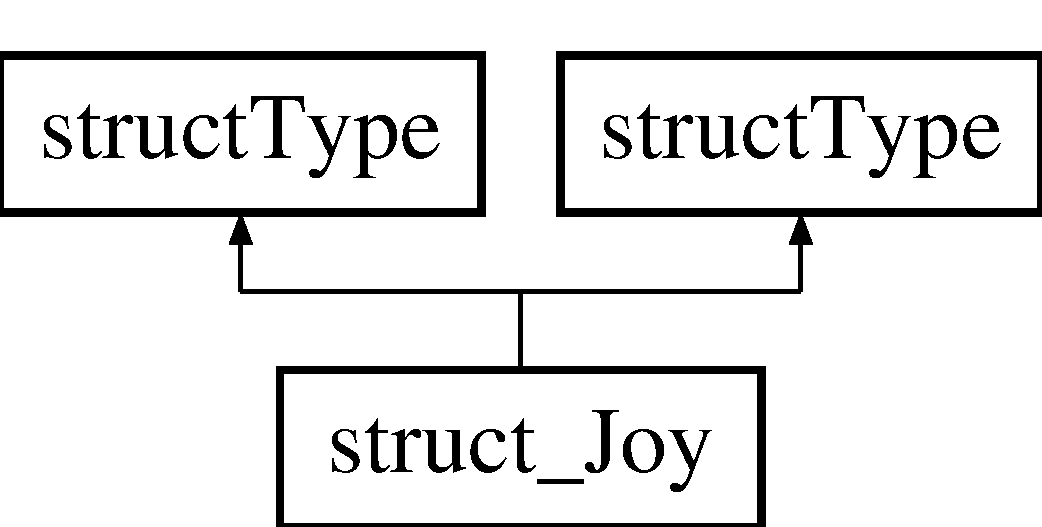
\includegraphics[height=2cm]{classstruct__Joy}
\end{center}
\end{figure}
\subsection*{Public Member Functions}
\begin{DoxyCompactItemize}
\item 
\hyperlink{classstruct__Joy_acd6825fe6adb60efa565e5ee22450255}{struct\_\-Joy} ()
\item 
char $\ast$ \hyperlink{classstruct__Joy_a85a218f4a0da41e33f9bf001c12c3a5a}{serialize} (char $\ast$maki)
\item 
char $\ast$ \hyperlink{classstruct__Joy_af683ec9dbedf3372b8ed17bff8c8b846}{Unserialize} (char $\ast$maki)
\item 
void \hyperlink{classstruct__Joy_a4d15e99a2fd78d6f162d0831ab4549f1}{storeData} (\hyperlink{structJoy}{Joy} $\ast$joy)
\item 
void $\ast$ \hyperlink{classstruct__Joy_a775c0f43b9125d8523ed26e72b6ebc44}{set\_\-Publisher} (char $\ast$name)
\item 
void $\ast$ \hyperlink{classstruct__Joy_a322d144fc1e42403ceb40f1e7f2b8536}{set\_\-Subscriber} (char $\ast$name)
\item 
void \hyperlink{classstruct__Joy_a0663befcb572431d8dc37cccc56bd6e5}{cmdVelCallback} (const joy::Joy::ConstPtr \&joy)
\item 
\hyperlink{classstruct__Joy_acd6825fe6adb60efa565e5ee22450255}{struct\_\-Joy} ()
\item 
char $\ast$ \hyperlink{classstruct__Joy_a0241cea32ad81ade99f9b484107e218d}{serialize} (char $\ast$maki)
\item 
char $\ast$ \hyperlink{classstruct__Joy_a6ad749ee0383dde28696e7aeeb050d09}{Unserialize} (char $\ast$maki)
\item 
void \hyperlink{classstruct__Joy_a4d15e99a2fd78d6f162d0831ab4549f1}{storeData} (\hyperlink{structJoy}{Joy} $\ast$joy)
\end{DoxyCompactItemize}
\subsection*{Public Attributes}
\begin{DoxyCompactItemize}
\item 
ros::NodeHandle \hyperlink{classstruct__Joy_afc0b4423d122753e49a142768882b458}{n}
\item 
ros::Publisher \hyperlink{classstruct__Joy_ae2f0324335e5f6692d1e398c80c84979}{joy\_\-pub}
\item 
ros::Subscriber \hyperlink{classstruct__Joy_ae01b03fd078106377cefb61eed252fde}{joy\_\-sub}
\item 
\hyperlink{structJoy}{Joy} \hyperlink{classstruct__Joy_a53d67349adb0afbdc4d30eead0903f21}{auxJoy1}
\item 
joy::Joy \hyperlink{classstruct__Joy_a1abf576689f865066505c7d3931cf175}{joy\_\-msg}
\item 
int \hyperlink{classstruct__Joy_a85b0158996d7206a23bf7012ceb23f9e}{sizeof\_\-Joy}
\item 
bool \hyperlink{classstruct__Joy_a350d227f222fa989e455d9ca0f28e106}{haveSubscriber}
\item 
bool \hyperlink{classstruct__Joy_a766b261da0d33afd7a1b0319be93b0cb}{havePublisher}
\end{DoxyCompactItemize}


\subsection{Constructor \& Destructor Documentation}
\hypertarget{classstruct__Joy_acd6825fe6adb60efa565e5ee22450255}{
\index{struct\_\-Joy@{struct\_\-Joy}!struct\_\-Joy@{struct\_\-Joy}}
\index{struct\_\-Joy@{struct\_\-Joy}!struct_Joy@{struct\_\-Joy}}
\subsubsection[{struct\_\-Joy}]{\setlength{\rightskip}{0pt plus 5cm}struct\_\-Joy::struct\_\-Joy ()}}
\label{classstruct__Joy_acd6825fe6adb60efa565e5ee22450255}
\hypertarget{classstruct__Joy_acd6825fe6adb60efa565e5ee22450255}{
\index{struct\_\-Joy@{struct\_\-Joy}!struct\_\-Joy@{struct\_\-Joy}}
\index{struct\_\-Joy@{struct\_\-Joy}!struct_Joy@{struct\_\-Joy}}
\subsubsection[{struct\_\-Joy}]{\setlength{\rightskip}{0pt plus 5cm}struct\_\-Joy::struct\_\-Joy ()}}
\label{classstruct__Joy_acd6825fe6adb60efa565e5ee22450255}


\subsection{Member Function Documentation}
\hypertarget{classstruct__Joy_a0663befcb572431d8dc37cccc56bd6e5}{
\index{struct\_\-Joy@{struct\_\-Joy}!cmdVelCallback@{cmdVelCallback}}
\index{cmdVelCallback@{cmdVelCallback}!struct_Joy@{struct\_\-Joy}}
\subsubsection[{cmdVelCallback}]{\setlength{\rightskip}{0pt plus 5cm}void struct\_\-Joy::cmdVelCallback (const joy::Joy::ConstPtr \& {\em joy})}}
\label{classstruct__Joy_a0663befcb572431d8dc37cccc56bd6e5}
\hypertarget{classstruct__Joy_a0241cea32ad81ade99f9b484107e218d}{
\index{struct\_\-Joy@{struct\_\-Joy}!serialize@{serialize}}
\index{serialize@{serialize}!struct_Joy@{struct\_\-Joy}}
\subsubsection[{serialize}]{\setlength{\rightskip}{0pt plus 5cm}char$\ast$ struct\_\-Joy::serialize (char $\ast$ {\em maki})\hspace{0.3cm}{\ttfamily  \mbox{[}virtual\mbox{]}}}}
\label{classstruct__Joy_a0241cea32ad81ade99f9b484107e218d}


Implements \hyperlink{classstructType_a515f5e08e2c7c054145d5dcce4e8adb1}{structType}.

\hypertarget{classstruct__Joy_a85a218f4a0da41e33f9bf001c12c3a5a}{
\index{struct\_\-Joy@{struct\_\-Joy}!serialize@{serialize}}
\index{serialize@{serialize}!struct_Joy@{struct\_\-Joy}}
\subsubsection[{serialize}]{\setlength{\rightskip}{0pt plus 5cm}char $\ast$ struct\_\-Joy::serialize (char $\ast$ {\em maki})\hspace{0.3cm}{\ttfamily  \mbox{[}virtual\mbox{]}}}}
\label{classstruct__Joy_a85a218f4a0da41e33f9bf001c12c3a5a}


Implements \hyperlink{classstructType_a515f5e08e2c7c054145d5dcce4e8adb1}{structType}.

\hypertarget{classstruct__Joy_a775c0f43b9125d8523ed26e72b6ebc44}{
\index{struct\_\-Joy@{struct\_\-Joy}!set\_\-Publisher@{set\_\-Publisher}}
\index{set\_\-Publisher@{set\_\-Publisher}!struct_Joy@{struct\_\-Joy}}
\subsubsection[{set\_\-Publisher}]{\setlength{\rightskip}{0pt plus 5cm}void $\ast$ struct\_\-Joy::set\_\-Publisher (char $\ast$ {\em name})\hspace{0.3cm}{\ttfamily  \mbox{[}virtual\mbox{]}}}}
\label{classstruct__Joy_a775c0f43b9125d8523ed26e72b6ebc44}


Implements \hyperlink{classstructType_aa017fe323160d25667ed838023db944d}{structType}.

\hypertarget{classstruct__Joy_a322d144fc1e42403ceb40f1e7f2b8536}{
\index{struct\_\-Joy@{struct\_\-Joy}!set\_\-Subscriber@{set\_\-Subscriber}}
\index{set\_\-Subscriber@{set\_\-Subscriber}!struct_Joy@{struct\_\-Joy}}
\subsubsection[{set\_\-Subscriber}]{\setlength{\rightskip}{0pt plus 5cm}void $\ast$ struct\_\-Joy::set\_\-Subscriber (char $\ast$ {\em name})\hspace{0.3cm}{\ttfamily  \mbox{[}virtual\mbox{]}}}}
\label{classstruct__Joy_a322d144fc1e42403ceb40f1e7f2b8536}


Implements \hyperlink{classstructType_a2f5adefc54e1e0f5a9100ab78e3c3749}{structType}.

\hypertarget{classstruct__Joy_a4d15e99a2fd78d6f162d0831ab4549f1}{
\index{struct\_\-Joy@{struct\_\-Joy}!storeData@{storeData}}
\index{storeData@{storeData}!struct_Joy@{struct\_\-Joy}}
\subsubsection[{storeData}]{\setlength{\rightskip}{0pt plus 5cm}void struct\_\-Joy::storeData ({\bf Joy} $\ast$ {\em joy})}}
\label{classstruct__Joy_a4d15e99a2fd78d6f162d0831ab4549f1}
\hypertarget{classstruct__Joy_a4d15e99a2fd78d6f162d0831ab4549f1}{
\index{struct\_\-Joy@{struct\_\-Joy}!storeData@{storeData}}
\index{storeData@{storeData}!struct_Joy@{struct\_\-Joy}}
\subsubsection[{storeData}]{\setlength{\rightskip}{0pt plus 5cm}void struct\_\-Joy::storeData ({\bf Joy} $\ast$ {\em joy})}}
\label{classstruct__Joy_a4d15e99a2fd78d6f162d0831ab4549f1}
\hypertarget{classstruct__Joy_a6ad749ee0383dde28696e7aeeb050d09}{
\index{struct\_\-Joy@{struct\_\-Joy}!Unserialize@{Unserialize}}
\index{Unserialize@{Unserialize}!struct_Joy@{struct\_\-Joy}}
\subsubsection[{Unserialize}]{\setlength{\rightskip}{0pt plus 5cm}char$\ast$ struct\_\-Joy::Unserialize (char $\ast$ {\em maki})\hspace{0.3cm}{\ttfamily  \mbox{[}virtual\mbox{]}}}}
\label{classstruct__Joy_a6ad749ee0383dde28696e7aeeb050d09}


Implements \hyperlink{classstructType_ac89681a3336b2fc76e65435238241db2}{structType}.

\hypertarget{classstruct__Joy_af683ec9dbedf3372b8ed17bff8c8b846}{
\index{struct\_\-Joy@{struct\_\-Joy}!Unserialize@{Unserialize}}
\index{Unserialize@{Unserialize}!struct_Joy@{struct\_\-Joy}}
\subsubsection[{Unserialize}]{\setlength{\rightskip}{0pt plus 5cm}char $\ast$ struct\_\-Joy::Unserialize (char $\ast$ {\em maki})\hspace{0.3cm}{\ttfamily  \mbox{[}virtual\mbox{]}}}}
\label{classstruct__Joy_af683ec9dbedf3372b8ed17bff8c8b846}


Implements \hyperlink{classstructType_ac89681a3336b2fc76e65435238241db2}{structType}.



\subsection{Member Data Documentation}
\hypertarget{classstruct__Joy_a53d67349adb0afbdc4d30eead0903f21}{
\index{struct\_\-Joy@{struct\_\-Joy}!auxJoy1@{auxJoy1}}
\index{auxJoy1@{auxJoy1}!struct_Joy@{struct\_\-Joy}}
\subsubsection[{auxJoy1}]{\setlength{\rightskip}{0pt plus 5cm}{\bf Joy} {\bf struct\_\-Joy::auxJoy1}}}
\label{classstruct__Joy_a53d67349adb0afbdc4d30eead0903f21}
\hypertarget{classstruct__Joy_a766b261da0d33afd7a1b0319be93b0cb}{
\index{struct\_\-Joy@{struct\_\-Joy}!havePublisher@{havePublisher}}
\index{havePublisher@{havePublisher}!struct_Joy@{struct\_\-Joy}}
\subsubsection[{havePublisher}]{\setlength{\rightskip}{0pt plus 5cm}bool {\bf struct\_\-Joy::havePublisher}}}
\label{classstruct__Joy_a766b261da0d33afd7a1b0319be93b0cb}
\hypertarget{classstruct__Joy_a350d227f222fa989e455d9ca0f28e106}{
\index{struct\_\-Joy@{struct\_\-Joy}!haveSubscriber@{haveSubscriber}}
\index{haveSubscriber@{haveSubscriber}!struct_Joy@{struct\_\-Joy}}
\subsubsection[{haveSubscriber}]{\setlength{\rightskip}{0pt plus 5cm}bool {\bf struct\_\-Joy::haveSubscriber}}}
\label{classstruct__Joy_a350d227f222fa989e455d9ca0f28e106}
\hypertarget{classstruct__Joy_a1abf576689f865066505c7d3931cf175}{
\index{struct\_\-Joy@{struct\_\-Joy}!joy\_\-msg@{joy\_\-msg}}
\index{joy\_\-msg@{joy\_\-msg}!struct_Joy@{struct\_\-Joy}}
\subsubsection[{joy\_\-msg}]{\setlength{\rightskip}{0pt plus 5cm}joy::Joy {\bf struct\_\-Joy::joy\_\-msg}}}
\label{classstruct__Joy_a1abf576689f865066505c7d3931cf175}
\hypertarget{classstruct__Joy_ae2f0324335e5f6692d1e398c80c84979}{
\index{struct\_\-Joy@{struct\_\-Joy}!joy\_\-pub@{joy\_\-pub}}
\index{joy\_\-pub@{joy\_\-pub}!struct_Joy@{struct\_\-Joy}}
\subsubsection[{joy\_\-pub}]{\setlength{\rightskip}{0pt plus 5cm}ros::Publisher {\bf struct\_\-Joy::joy\_\-pub}}}
\label{classstruct__Joy_ae2f0324335e5f6692d1e398c80c84979}
\hypertarget{classstruct__Joy_ae01b03fd078106377cefb61eed252fde}{
\index{struct\_\-Joy@{struct\_\-Joy}!joy\_\-sub@{joy\_\-sub}}
\index{joy\_\-sub@{joy\_\-sub}!struct_Joy@{struct\_\-Joy}}
\subsubsection[{joy\_\-sub}]{\setlength{\rightskip}{0pt plus 5cm}ros::Subscriber {\bf struct\_\-Joy::joy\_\-sub}}}
\label{classstruct__Joy_ae01b03fd078106377cefb61eed252fde}
\hypertarget{classstruct__Joy_afc0b4423d122753e49a142768882b458}{
\index{struct\_\-Joy@{struct\_\-Joy}!n@{n}}
\index{n@{n}!struct_Joy@{struct\_\-Joy}}
\subsubsection[{n}]{\setlength{\rightskip}{0pt plus 5cm}ros::NodeHandle {\bf struct\_\-Joy::n}}}
\label{classstruct__Joy_afc0b4423d122753e49a142768882b458}
\hypertarget{classstruct__Joy_a85b0158996d7206a23bf7012ceb23f9e}{
\index{struct\_\-Joy@{struct\_\-Joy}!sizeof\_\-Joy@{sizeof\_\-Joy}}
\index{sizeof\_\-Joy@{sizeof\_\-Joy}!struct_Joy@{struct\_\-Joy}}
\subsubsection[{sizeof\_\-Joy}]{\setlength{\rightskip}{0pt plus 5cm}int {\bf struct\_\-Joy::sizeof\_\-Joy}}}
\label{classstruct__Joy_a85b0158996d7206a23bf7012ceb23f9e}


The documentation for this class was generated from the following files:\begin{DoxyCompactItemize}
\item 
include/TCP\_\-RTAI/\hyperlink{AaronMR__C_8hpp}{AaronMR\_\-C.hpp}\item 
include/TCP\_\-RTAI/\hyperlink{AaronMR__S_8hpp}{AaronMR\_\-S.hpp}\item 
include/TCP\_\-RTAI/\hyperlink{AaronMR__C_8cpp}{AaronMR\_\-C.cpp}\item 
include/TCP\_\-RTAI/\hyperlink{AaronMR__S_8cpp}{AaronMR\_\-S.cpp}\end{DoxyCompactItemize}

\hypertarget{classstruct__Twist}{
\section{struct\_\-Twist Class Reference}
\label{classstruct__Twist}\index{struct\_\-Twist@{struct\_\-Twist}}
}


{\ttfamily \#include $<$AaronMR\_\-C.hpp$>$}

Inheritance diagram for struct\_\-Twist:\begin{figure}[H]
\begin{center}
\leavevmode
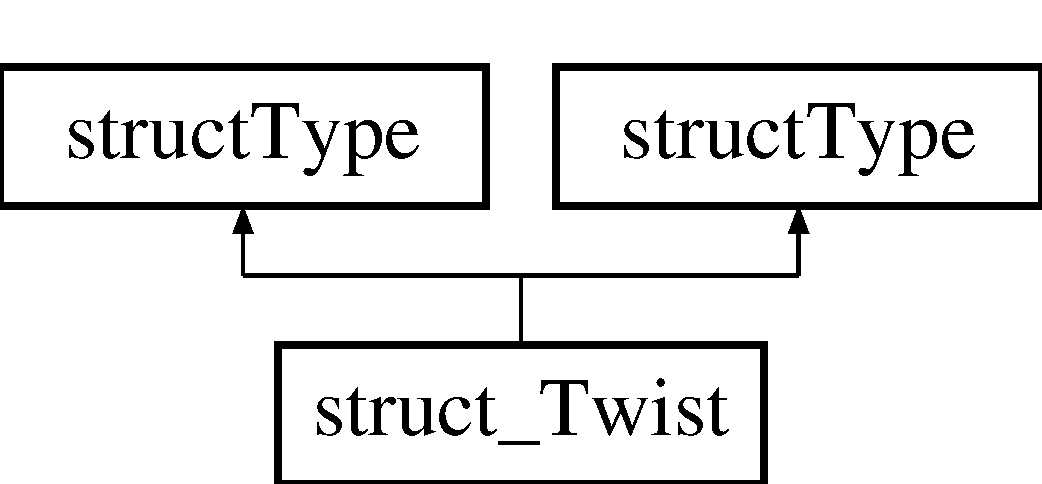
\includegraphics[height=2cm]{classstruct__Twist}
\end{center}
\end{figure}
\subsection*{Public Member Functions}
\begin{DoxyCompactItemize}
\item 
\hyperlink{classstruct__Twist_a164175a79d7c3c66dbd7fdbcea350029}{struct\_\-Twist} ()
\item 
char $\ast$ \hyperlink{classstruct__Twist_aee6e94e0914c89920f211a04b5ad4f9f}{serialize} (char $\ast$maki)
\item 
char $\ast$ \hyperlink{classstruct__Twist_a0531691876c9cbabb1932cb54592c956}{Unserialize} (char $\ast$maki)
\item 
void \hyperlink{classstruct__Twist_a0385da1a9307377c97fd0bee2c94f1f6}{storeData} (\hyperlink{structJoy}{Joy} $\ast$joy)
\item 
void $\ast$ \hyperlink{classstruct__Twist_adb9080f278fb0608806c42156f1f9d69}{set\_\-Publisher} (char $\ast$name)
\item 
void $\ast$ \hyperlink{classstruct__Twist_ae87a3d1851c29e2707ae7bd35fac323b}{set\_\-Subscriber} (char $\ast$name)
\item 
void \hyperlink{classstruct__Twist_aa4b5acddd72e4b9766989bd9be5e2285}{cmdVelCallback} (const geometry\_\-msgs::Twist \&joy)
\item 
\hyperlink{classstruct__Twist_a164175a79d7c3c66dbd7fdbcea350029}{struct\_\-Twist} ()
\item 
char $\ast$ \hyperlink{classstruct__Twist_afc5c6e9e092a700e3906e67d7918d4ab}{serialize} (char $\ast$maki)
\item 
char $\ast$ \hyperlink{classstruct__Twist_a69b1008d4218c372a14b7ce1e8d6d485}{Unserialize} (char $\ast$maki)
\item 
void \hyperlink{classstruct__Twist_a0385da1a9307377c97fd0bee2c94f1f6}{storeData} (\hyperlink{structJoy}{Joy} $\ast$joy)
\end{DoxyCompactItemize}
\subsection*{Public Attributes}
\begin{DoxyCompactItemize}
\item 
ros::NodeHandle \hyperlink{classstruct__Twist_a2d3e2346abef34de6bb72a5b783a367e}{n}
\item 
ros::Publisher \hyperlink{classstruct__Twist_aee5b5a8a8f139c8d94c50ea74aa242df}{twist\_\-pub}
\item 
ros::Subscriber \hyperlink{classstruct__Twist_aec635faa1bd8d788f567f7fdfe425dfb}{twist\_\-sub}
\item 
\hyperlink{structJoy}{Joy} \hyperlink{classstruct__Twist_a62e055e979ef7e00e4fa5b28e5af58a3}{auxJoy1}
\item 
joy::Joy \hyperlink{classstruct__Twist_a71712cfdc47912e38edf31527ddabdf0}{joy\_\-msg}
\item 
geometry\_\-msgs::Twist \hyperlink{classstruct__Twist_a9df8e9fe3a53331a21e015a7a68346f1}{twist\_\-}
\item 
int \hyperlink{classstruct__Twist_af6f8a2260faa75ff5e69195ea06dbdc5}{sizeof\_\-Joy}
\item 
bool \hyperlink{classstruct__Twist_af4ebb0d68d02c7e0bc6f4ef01a28f3f9}{haveSubscriber}
\item 
bool \hyperlink{classstruct__Twist_a56123bf7b16afa13ca976101c263f9e1}{havePublisher}
\end{DoxyCompactItemize}


\subsection{Constructor \& Destructor Documentation}
\hypertarget{classstruct__Twist_a164175a79d7c3c66dbd7fdbcea350029}{
\index{struct\_\-Twist@{struct\_\-Twist}!struct\_\-Twist@{struct\_\-Twist}}
\index{struct\_\-Twist@{struct\_\-Twist}!struct_Twist@{struct\_\-Twist}}
\subsubsection[{struct\_\-Twist}]{\setlength{\rightskip}{0pt plus 5cm}struct\_\-Twist::struct\_\-Twist ()}}
\label{classstruct__Twist_a164175a79d7c3c66dbd7fdbcea350029}
\hypertarget{classstruct__Twist_a164175a79d7c3c66dbd7fdbcea350029}{
\index{struct\_\-Twist@{struct\_\-Twist}!struct\_\-Twist@{struct\_\-Twist}}
\index{struct\_\-Twist@{struct\_\-Twist}!struct_Twist@{struct\_\-Twist}}
\subsubsection[{struct\_\-Twist}]{\setlength{\rightskip}{0pt plus 5cm}struct\_\-Twist::struct\_\-Twist ()}}
\label{classstruct__Twist_a164175a79d7c3c66dbd7fdbcea350029}


\subsection{Member Function Documentation}
\hypertarget{classstruct__Twist_aa4b5acddd72e4b9766989bd9be5e2285}{
\index{struct\_\-Twist@{struct\_\-Twist}!cmdVelCallback@{cmdVelCallback}}
\index{cmdVelCallback@{cmdVelCallback}!struct_Twist@{struct\_\-Twist}}
\subsubsection[{cmdVelCallback}]{\setlength{\rightskip}{0pt plus 5cm}void struct\_\-Twist::cmdVelCallback (const geometry\_\-msgs::Twist \& {\em joy})}}
\label{classstruct__Twist_aa4b5acddd72e4b9766989bd9be5e2285}
\hypertarget{classstruct__Twist_afc5c6e9e092a700e3906e67d7918d4ab}{
\index{struct\_\-Twist@{struct\_\-Twist}!serialize@{serialize}}
\index{serialize@{serialize}!struct_Twist@{struct\_\-Twist}}
\subsubsection[{serialize}]{\setlength{\rightskip}{0pt plus 5cm}char$\ast$ struct\_\-Twist::serialize (char $\ast$ {\em maki})\hspace{0.3cm}{\ttfamily  \mbox{[}virtual\mbox{]}}}}
\label{classstruct__Twist_afc5c6e9e092a700e3906e67d7918d4ab}


Implements \hyperlink{classstructType_a515f5e08e2c7c054145d5dcce4e8adb1}{structType}.

\hypertarget{classstruct__Twist_aee6e94e0914c89920f211a04b5ad4f9f}{
\index{struct\_\-Twist@{struct\_\-Twist}!serialize@{serialize}}
\index{serialize@{serialize}!struct_Twist@{struct\_\-Twist}}
\subsubsection[{serialize}]{\setlength{\rightskip}{0pt plus 5cm}char $\ast$ struct\_\-Twist::serialize (char $\ast$ {\em maki})\hspace{0.3cm}{\ttfamily  \mbox{[}virtual\mbox{]}}}}
\label{classstruct__Twist_aee6e94e0914c89920f211a04b5ad4f9f}


Implements \hyperlink{classstructType_a515f5e08e2c7c054145d5dcce4e8adb1}{structType}.

\hypertarget{classstruct__Twist_adb9080f278fb0608806c42156f1f9d69}{
\index{struct\_\-Twist@{struct\_\-Twist}!set\_\-Publisher@{set\_\-Publisher}}
\index{set\_\-Publisher@{set\_\-Publisher}!struct_Twist@{struct\_\-Twist}}
\subsubsection[{set\_\-Publisher}]{\setlength{\rightskip}{0pt plus 5cm}void $\ast$ struct\_\-Twist::set\_\-Publisher (char $\ast$ {\em name})\hspace{0.3cm}{\ttfamily  \mbox{[}virtual\mbox{]}}}}
\label{classstruct__Twist_adb9080f278fb0608806c42156f1f9d69}


Implements \hyperlink{classstructType_aa017fe323160d25667ed838023db944d}{structType}.

\hypertarget{classstruct__Twist_ae87a3d1851c29e2707ae7bd35fac323b}{
\index{struct\_\-Twist@{struct\_\-Twist}!set\_\-Subscriber@{set\_\-Subscriber}}
\index{set\_\-Subscriber@{set\_\-Subscriber}!struct_Twist@{struct\_\-Twist}}
\subsubsection[{set\_\-Subscriber}]{\setlength{\rightskip}{0pt plus 5cm}void $\ast$ struct\_\-Twist::set\_\-Subscriber (char $\ast$ {\em name})\hspace{0.3cm}{\ttfamily  \mbox{[}virtual\mbox{]}}}}
\label{classstruct__Twist_ae87a3d1851c29e2707ae7bd35fac323b}


Implements \hyperlink{classstructType_a2f5adefc54e1e0f5a9100ab78e3c3749}{structType}.

\hypertarget{classstruct__Twist_a0385da1a9307377c97fd0bee2c94f1f6}{
\index{struct\_\-Twist@{struct\_\-Twist}!storeData@{storeData}}
\index{storeData@{storeData}!struct_Twist@{struct\_\-Twist}}
\subsubsection[{storeData}]{\setlength{\rightskip}{0pt plus 5cm}void struct\_\-Twist::storeData ({\bf Joy} $\ast$ {\em joy})}}
\label{classstruct__Twist_a0385da1a9307377c97fd0bee2c94f1f6}
\hypertarget{classstruct__Twist_a0385da1a9307377c97fd0bee2c94f1f6}{
\index{struct\_\-Twist@{struct\_\-Twist}!storeData@{storeData}}
\index{storeData@{storeData}!struct_Twist@{struct\_\-Twist}}
\subsubsection[{storeData}]{\setlength{\rightskip}{0pt plus 5cm}void struct\_\-Twist::storeData ({\bf Joy} $\ast$ {\em joy})}}
\label{classstruct__Twist_a0385da1a9307377c97fd0bee2c94f1f6}
\hypertarget{classstruct__Twist_a69b1008d4218c372a14b7ce1e8d6d485}{
\index{struct\_\-Twist@{struct\_\-Twist}!Unserialize@{Unserialize}}
\index{Unserialize@{Unserialize}!struct_Twist@{struct\_\-Twist}}
\subsubsection[{Unserialize}]{\setlength{\rightskip}{0pt plus 5cm}char$\ast$ struct\_\-Twist::Unserialize (char $\ast$ {\em maki})\hspace{0.3cm}{\ttfamily  \mbox{[}virtual\mbox{]}}}}
\label{classstruct__Twist_a69b1008d4218c372a14b7ce1e8d6d485}


Implements \hyperlink{classstructType_ac89681a3336b2fc76e65435238241db2}{structType}.

\hypertarget{classstruct__Twist_a0531691876c9cbabb1932cb54592c956}{
\index{struct\_\-Twist@{struct\_\-Twist}!Unserialize@{Unserialize}}
\index{Unserialize@{Unserialize}!struct_Twist@{struct\_\-Twist}}
\subsubsection[{Unserialize}]{\setlength{\rightskip}{0pt plus 5cm}char $\ast$ struct\_\-Twist::Unserialize (char $\ast$ {\em maki})\hspace{0.3cm}{\ttfamily  \mbox{[}virtual\mbox{]}}}}
\label{classstruct__Twist_a0531691876c9cbabb1932cb54592c956}


Implements \hyperlink{classstructType_ac89681a3336b2fc76e65435238241db2}{structType}.



\subsection{Member Data Documentation}
\hypertarget{classstruct__Twist_a62e055e979ef7e00e4fa5b28e5af58a3}{
\index{struct\_\-Twist@{struct\_\-Twist}!auxJoy1@{auxJoy1}}
\index{auxJoy1@{auxJoy1}!struct_Twist@{struct\_\-Twist}}
\subsubsection[{auxJoy1}]{\setlength{\rightskip}{0pt plus 5cm}{\bf Joy} {\bf struct\_\-Twist::auxJoy1}}}
\label{classstruct__Twist_a62e055e979ef7e00e4fa5b28e5af58a3}
\hypertarget{classstruct__Twist_a56123bf7b16afa13ca976101c263f9e1}{
\index{struct\_\-Twist@{struct\_\-Twist}!havePublisher@{havePublisher}}
\index{havePublisher@{havePublisher}!struct_Twist@{struct\_\-Twist}}
\subsubsection[{havePublisher}]{\setlength{\rightskip}{0pt plus 5cm}bool {\bf struct\_\-Twist::havePublisher}}}
\label{classstruct__Twist_a56123bf7b16afa13ca976101c263f9e1}
\hypertarget{classstruct__Twist_af4ebb0d68d02c7e0bc6f4ef01a28f3f9}{
\index{struct\_\-Twist@{struct\_\-Twist}!haveSubscriber@{haveSubscriber}}
\index{haveSubscriber@{haveSubscriber}!struct_Twist@{struct\_\-Twist}}
\subsubsection[{haveSubscriber}]{\setlength{\rightskip}{0pt plus 5cm}bool {\bf struct\_\-Twist::haveSubscriber}}}
\label{classstruct__Twist_af4ebb0d68d02c7e0bc6f4ef01a28f3f9}
\hypertarget{classstruct__Twist_a71712cfdc47912e38edf31527ddabdf0}{
\index{struct\_\-Twist@{struct\_\-Twist}!joy\_\-msg@{joy\_\-msg}}
\index{joy\_\-msg@{joy\_\-msg}!struct_Twist@{struct\_\-Twist}}
\subsubsection[{joy\_\-msg}]{\setlength{\rightskip}{0pt plus 5cm}joy::Joy {\bf struct\_\-Twist::joy\_\-msg}}}
\label{classstruct__Twist_a71712cfdc47912e38edf31527ddabdf0}
\hypertarget{classstruct__Twist_a2d3e2346abef34de6bb72a5b783a367e}{
\index{struct\_\-Twist@{struct\_\-Twist}!n@{n}}
\index{n@{n}!struct_Twist@{struct\_\-Twist}}
\subsubsection[{n}]{\setlength{\rightskip}{0pt plus 5cm}ros::NodeHandle {\bf struct\_\-Twist::n}}}
\label{classstruct__Twist_a2d3e2346abef34de6bb72a5b783a367e}
\hypertarget{classstruct__Twist_af6f8a2260faa75ff5e69195ea06dbdc5}{
\index{struct\_\-Twist@{struct\_\-Twist}!sizeof\_\-Joy@{sizeof\_\-Joy}}
\index{sizeof\_\-Joy@{sizeof\_\-Joy}!struct_Twist@{struct\_\-Twist}}
\subsubsection[{sizeof\_\-Joy}]{\setlength{\rightskip}{0pt plus 5cm}int {\bf struct\_\-Twist::sizeof\_\-Joy}}}
\label{classstruct__Twist_af6f8a2260faa75ff5e69195ea06dbdc5}
\hypertarget{classstruct__Twist_a9df8e9fe3a53331a21e015a7a68346f1}{
\index{struct\_\-Twist@{struct\_\-Twist}!twist\_\-@{twist\_\-}}
\index{twist\_\-@{twist\_\-}!struct_Twist@{struct\_\-Twist}}
\subsubsection[{twist\_\-}]{\setlength{\rightskip}{0pt plus 5cm}geometry\_\-msgs::Twist {\bf struct\_\-Twist::twist\_\-}}}
\label{classstruct__Twist_a9df8e9fe3a53331a21e015a7a68346f1}
\hypertarget{classstruct__Twist_aee5b5a8a8f139c8d94c50ea74aa242df}{
\index{struct\_\-Twist@{struct\_\-Twist}!twist\_\-pub@{twist\_\-pub}}
\index{twist\_\-pub@{twist\_\-pub}!struct_Twist@{struct\_\-Twist}}
\subsubsection[{twist\_\-pub}]{\setlength{\rightskip}{0pt plus 5cm}ros::Publisher {\bf struct\_\-Twist::twist\_\-pub}}}
\label{classstruct__Twist_aee5b5a8a8f139c8d94c50ea74aa242df}
\hypertarget{classstruct__Twist_aec635faa1bd8d788f567f7fdfe425dfb}{
\index{struct\_\-Twist@{struct\_\-Twist}!twist\_\-sub@{twist\_\-sub}}
\index{twist\_\-sub@{twist\_\-sub}!struct_Twist@{struct\_\-Twist}}
\subsubsection[{twist\_\-sub}]{\setlength{\rightskip}{0pt plus 5cm}ros::Subscriber {\bf struct\_\-Twist::twist\_\-sub}}}
\label{classstruct__Twist_aec635faa1bd8d788f567f7fdfe425dfb}


The documentation for this class was generated from the following files:\begin{DoxyCompactItemize}
\item 
include/TCP\_\-RTAI/\hyperlink{AaronMR__C_8hpp}{AaronMR\_\-C.hpp}\item 
include/TCP\_\-RTAI/\hyperlink{AaronMR__S_8hpp}{AaronMR\_\-S.hpp}\item 
include/TCP\_\-RTAI/\hyperlink{AaronMR__C_8cpp}{AaronMR\_\-C.cpp}\item 
include/TCP\_\-RTAI/\hyperlink{AaronMR__S_8cpp}{AaronMR\_\-S.cpp}\end{DoxyCompactItemize}

\hypertarget{classstructType}{
\section{structType Class Reference}
\label{classstructType}\index{structType@{structType}}
}


{\ttfamily \#include $<$AaronMR\_\-C.hpp$>$}

Inheritance diagram for structType:\begin{figure}[H]
\begin{center}
\leavevmode
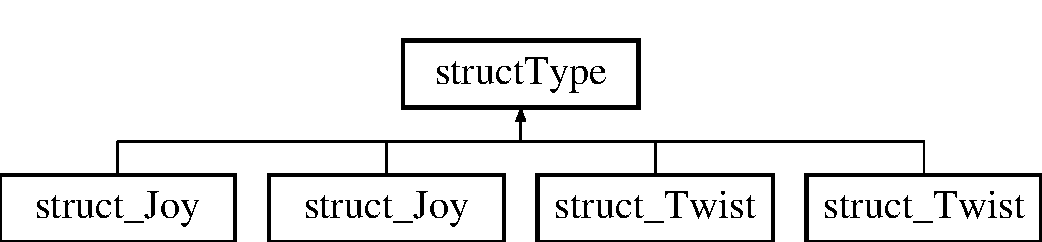
\includegraphics[height=2cm]{classstructType}
\end{center}
\end{figure}
\subsection*{Public Member Functions}
\begin{DoxyCompactItemize}
\item 
virtual char $\ast$ \hyperlink{classstructType_a515f5e08e2c7c054145d5dcce4e8adb1}{serialize} (char $\ast$maki)=0
\item 
virtual char $\ast$ \hyperlink{classstructType_ac89681a3336b2fc76e65435238241db2}{Unserialize} (char $\ast$maki)=0
\item 
virtual void $\ast$ \hyperlink{classstructType_aa017fe323160d25667ed838023db944d}{set\_\-Publisher} (char $\ast$name)=0
\item 
virtual void $\ast$ \hyperlink{classstructType_a2f5adefc54e1e0f5a9100ab78e3c3749}{set\_\-Subscriber} (char $\ast$name)=0
\item 
void \hyperlink{classstructType_aeeef09e0813fb532bd84bbd8010bdd94}{storeData} ()
\item 
virtual char $\ast$ \hyperlink{classstructType_a515f5e08e2c7c054145d5dcce4e8adb1}{serialize} (char $\ast$maki)=0
\item 
virtual char $\ast$ \hyperlink{classstructType_ac89681a3336b2fc76e65435238241db2}{Unserialize} (char $\ast$maki)=0
\item 
void \hyperlink{classstructType_aeeef09e0813fb532bd84bbd8010bdd94}{storeData} ()
\end{DoxyCompactItemize}


\subsection{Member Function Documentation}
\hypertarget{classstructType_a515f5e08e2c7c054145d5dcce4e8adb1}{
\index{structType@{structType}!serialize@{serialize}}
\index{serialize@{serialize}!structType@{structType}}
\subsubsection[{serialize}]{\setlength{\rightskip}{0pt plus 5cm}virtual char$\ast$ structType::serialize (char $\ast$ {\em maki})\hspace{0.3cm}{\ttfamily  \mbox{[}pure virtual\mbox{]}}}}
\label{classstructType_a515f5e08e2c7c054145d5dcce4e8adb1}


Implemented in \hyperlink{classstruct__Joy_a85a218f4a0da41e33f9bf001c12c3a5a}{struct\_\-Joy}, \hyperlink{classstruct__Twist_aee6e94e0914c89920f211a04b5ad4f9f}{struct\_\-Twist}, \hyperlink{classstruct__Joy_a0241cea32ad81ade99f9b484107e218d}{struct\_\-Joy}, and \hyperlink{classstruct__Twist_afc5c6e9e092a700e3906e67d7918d4ab}{struct\_\-Twist}.

\hypertarget{classstructType_a515f5e08e2c7c054145d5dcce4e8adb1}{
\index{structType@{structType}!serialize@{serialize}}
\index{serialize@{serialize}!structType@{structType}}
\subsubsection[{serialize}]{\setlength{\rightskip}{0pt plus 5cm}virtual char$\ast$ structType::serialize (char $\ast$ {\em maki})\hspace{0.3cm}{\ttfamily  \mbox{[}pure virtual\mbox{]}}}}
\label{classstructType_a515f5e08e2c7c054145d5dcce4e8adb1}


Implemented in \hyperlink{classstruct__Joy_a85a218f4a0da41e33f9bf001c12c3a5a}{struct\_\-Joy}, \hyperlink{classstruct__Twist_aee6e94e0914c89920f211a04b5ad4f9f}{struct\_\-Twist}, \hyperlink{classstruct__Joy_a0241cea32ad81ade99f9b484107e218d}{struct\_\-Joy}, and \hyperlink{classstruct__Twist_afc5c6e9e092a700e3906e67d7918d4ab}{struct\_\-Twist}.

\hypertarget{classstructType_aa017fe323160d25667ed838023db944d}{
\index{structType@{structType}!set\_\-Publisher@{set\_\-Publisher}}
\index{set\_\-Publisher@{set\_\-Publisher}!structType@{structType}}
\subsubsection[{set\_\-Publisher}]{\setlength{\rightskip}{0pt plus 5cm}virtual void$\ast$ structType::set\_\-Publisher (char $\ast$ {\em name})\hspace{0.3cm}{\ttfamily  \mbox{[}pure virtual\mbox{]}}}}
\label{classstructType_aa017fe323160d25667ed838023db944d}


Implemented in \hyperlink{classstruct__Joy_a775c0f43b9125d8523ed26e72b6ebc44}{struct\_\-Joy}, and \hyperlink{classstruct__Twist_adb9080f278fb0608806c42156f1f9d69}{struct\_\-Twist}.

\hypertarget{classstructType_a2f5adefc54e1e0f5a9100ab78e3c3749}{
\index{structType@{structType}!set\_\-Subscriber@{set\_\-Subscriber}}
\index{set\_\-Subscriber@{set\_\-Subscriber}!structType@{structType}}
\subsubsection[{set\_\-Subscriber}]{\setlength{\rightskip}{0pt plus 5cm}virtual void$\ast$ structType::set\_\-Subscriber (char $\ast$ {\em name})\hspace{0.3cm}{\ttfamily  \mbox{[}pure virtual\mbox{]}}}}
\label{classstructType_a2f5adefc54e1e0f5a9100ab78e3c3749}


Implemented in \hyperlink{classstruct__Joy_a322d144fc1e42403ceb40f1e7f2b8536}{struct\_\-Joy}, and \hyperlink{classstruct__Twist_ae87a3d1851c29e2707ae7bd35fac323b}{struct\_\-Twist}.

\hypertarget{classstructType_aeeef09e0813fb532bd84bbd8010bdd94}{
\index{structType@{structType}!storeData@{storeData}}
\index{storeData@{storeData}!structType@{structType}}
\subsubsection[{storeData}]{\setlength{\rightskip}{0pt plus 5cm}void structType::storeData ()}}
\label{classstructType_aeeef09e0813fb532bd84bbd8010bdd94}
\hypertarget{classstructType_aeeef09e0813fb532bd84bbd8010bdd94}{
\index{structType@{structType}!storeData@{storeData}}
\index{storeData@{storeData}!structType@{structType}}
\subsubsection[{storeData}]{\setlength{\rightskip}{0pt plus 5cm}void structType::storeData ()}}
\label{classstructType_aeeef09e0813fb532bd84bbd8010bdd94}
\hypertarget{classstructType_ac89681a3336b2fc76e65435238241db2}{
\index{structType@{structType}!Unserialize@{Unserialize}}
\index{Unserialize@{Unserialize}!structType@{structType}}
\subsubsection[{Unserialize}]{\setlength{\rightskip}{0pt plus 5cm}virtual char$\ast$ structType::Unserialize (char $\ast$ {\em maki})\hspace{0.3cm}{\ttfamily  \mbox{[}pure virtual\mbox{]}}}}
\label{classstructType_ac89681a3336b2fc76e65435238241db2}


Implemented in \hyperlink{classstruct__Joy_af683ec9dbedf3372b8ed17bff8c8b846}{struct\_\-Joy}, \hyperlink{classstruct__Twist_a0531691876c9cbabb1932cb54592c956}{struct\_\-Twist}, \hyperlink{classstruct__Joy_a6ad749ee0383dde28696e7aeeb050d09}{struct\_\-Joy}, and \hyperlink{classstruct__Twist_a69b1008d4218c372a14b7ce1e8d6d485}{struct\_\-Twist}.

\hypertarget{classstructType_ac89681a3336b2fc76e65435238241db2}{
\index{structType@{structType}!Unserialize@{Unserialize}}
\index{Unserialize@{Unserialize}!structType@{structType}}
\subsubsection[{Unserialize}]{\setlength{\rightskip}{0pt plus 5cm}virtual char$\ast$ structType::Unserialize (char $\ast$ {\em maki})\hspace{0.3cm}{\ttfamily  \mbox{[}pure virtual\mbox{]}}}}
\label{classstructType_ac89681a3336b2fc76e65435238241db2}


Implemented in \hyperlink{classstruct__Joy_af683ec9dbedf3372b8ed17bff8c8b846}{struct\_\-Joy}, \hyperlink{classstruct__Twist_a0531691876c9cbabb1932cb54592c956}{struct\_\-Twist}, \hyperlink{classstruct__Joy_a6ad749ee0383dde28696e7aeeb050d09}{struct\_\-Joy}, and \hyperlink{classstruct__Twist_a69b1008d4218c372a14b7ce1e8d6d485}{struct\_\-Twist}.



The documentation for this class was generated from the following files:\begin{DoxyCompactItemize}
\item 
include/TCP\_\-RTAI/\hyperlink{AaronMR__C_8hpp}{AaronMR\_\-C.hpp}\item 
include/TCP\_\-RTAI/\hyperlink{AaronMR__S_8hpp}{AaronMR\_\-S.hpp}\end{DoxyCompactItemize}

\hypertarget{classtransmision}{
\section{transmision Class Reference}
\label{classtransmision}\index{transmision@{transmision}}
}


{\ttfamily \#include $<$transmition.h$>$}

\subsection*{Public Member Functions}
\begin{DoxyCompactItemize}
\item 
\hyperlink{classtransmision_a9cbd838625edd4d839b03bc1236a2ca2}{transmision} (int aux)
\item 
\hyperlink{classtransmision_ae7d8d3fccee4ddb493e97061c5811cad}{$\sim$transmision} ()
\item 
int \hyperlink{classtransmision_aafa9957efe4d2fc1472a5b298650122d}{sendData} (\hyperlink{structStruct__1}{Struct\_\-1} $\ast$a)
\item 
int \hyperlink{classtransmision_a1dbf734bad68289da9ec9bf0b28000f7}{recvData} (\hyperlink{structStruct__1}{Struct\_\-1} $\ast$a)
\item 
int \hyperlink{classtransmision_a30a3f43077162e430096e9415749d31c}{sendData} (\hyperlink{structStruct__2}{Struct\_\-2} $\ast$b)
\item 
int \hyperlink{classtransmision_a905e696047472384fdd47c962be55e72}{recvData} (\hyperlink{structStruct__2}{Struct\_\-2} $\ast$b)
\item 
int \hyperlink{classtransmision_a1d6f5d22ea3139d9580bd489e78c15b5}{sendData} (\hyperlink{structStruct__3}{Struct\_\-3} $\ast$c)
\item 
int \hyperlink{classtransmision_a81218832d0a18422027503d1b529ac3c}{recvData} (\hyperlink{structStruct__3}{Struct\_\-3} $\ast$c)
\item 
int \hyperlink{classtransmision_a07a6ca5245553367f31662bb9ae9ce5c}{sendData} (\hyperlink{structJoy}{Joy} $\ast$joy)
\item 
int \hyperlink{classtransmision_ab200238f23c207a2acdcbfa44facf5ba}{recvData} (\hyperlink{structJoy}{Joy} $\ast$joy)
\item 
int \hyperlink{classtransmision_af76f07480f2cb76eedc2d3db45bd3aa0}{sendData} (char $\ast$buffer)
\item 
int \hyperlink{classtransmision_a1af0251c8c9487dc6feff1075bb7bee2}{recvData} (char $\ast$buffer)
\item 
int \hyperlink{classtransmision_a23c12d04eab4a7bd583a3b376c4c8fd3}{sendData} (\hyperlink{structTwist}{Twist} $\ast$twist)
\item 
int \hyperlink{classtransmision_a89c0adf9833c7d42be1fcd1c7dc978e0}{recvData} (\hyperlink{structTwist}{Twist} $\ast$twist)
\item 
int \hyperlink{classtransmision_a383ce5304c45dc09b7c994b9708dc6b2}{sendData} (\hyperlink{structOdometry}{Odometry} $\ast$odometry)
\item 
int \hyperlink{classtransmision_ad1079ca1013063468528715ded83851e}{recvData} (\hyperlink{structOdometry}{Odometry} $\ast$odometry)
\end{DoxyCompactItemize}
\subsection*{Public Attributes}
\begin{DoxyCompactItemize}
\item 
int \hyperlink{classtransmision_a3852938bfe54a2b913a7965824fb2acf}{sock}
\end{DoxyCompactItemize}


\subsection{Constructor \& Destructor Documentation}
\hypertarget{classtransmision_a9cbd838625edd4d839b03bc1236a2ca2}{
\index{transmision@{transmision}!transmision@{transmision}}
\index{transmision@{transmision}!transmision@{transmision}}
\subsubsection[{transmision}]{\setlength{\rightskip}{0pt plus 5cm}transmision::transmision (int {\em aux})}}
\label{classtransmision_a9cbd838625edd4d839b03bc1236a2ca2}
\hypertarget{classtransmision_ae7d8d3fccee4ddb493e97061c5811cad}{
\index{transmision@{transmision}!$\sim$transmision@{$\sim$transmision}}
\index{$\sim$transmision@{$\sim$transmision}!transmision@{transmision}}
\subsubsection[{$\sim$transmision}]{\setlength{\rightskip}{0pt plus 5cm}transmision::$\sim$transmision ()}}
\label{classtransmision_ae7d8d3fccee4ddb493e97061c5811cad}


\subsection{Member Function Documentation}
\hypertarget{classtransmision_ad1079ca1013063468528715ded83851e}{
\index{transmision@{transmision}!recvData@{recvData}}
\index{recvData@{recvData}!transmision@{transmision}}
\subsubsection[{recvData}]{\setlength{\rightskip}{0pt plus 5cm}int transmision::recvData ({\bf Odometry} $\ast$ {\em odometry})}}
\label{classtransmision_ad1079ca1013063468528715ded83851e}
\hypertarget{classtransmision_a89c0adf9833c7d42be1fcd1c7dc978e0}{
\index{transmision@{transmision}!recvData@{recvData}}
\index{recvData@{recvData}!transmision@{transmision}}
\subsubsection[{recvData}]{\setlength{\rightskip}{0pt plus 5cm}int transmision::recvData ({\bf Twist} $\ast$ {\em twist})}}
\label{classtransmision_a89c0adf9833c7d42be1fcd1c7dc978e0}
\hypertarget{classtransmision_a1af0251c8c9487dc6feff1075bb7bee2}{
\index{transmision@{transmision}!recvData@{recvData}}
\index{recvData@{recvData}!transmision@{transmision}}
\subsubsection[{recvData}]{\setlength{\rightskip}{0pt plus 5cm}int transmision::recvData (char $\ast$ {\em buffer})}}
\label{classtransmision_a1af0251c8c9487dc6feff1075bb7bee2}
\hypertarget{classtransmision_ab200238f23c207a2acdcbfa44facf5ba}{
\index{transmision@{transmision}!recvData@{recvData}}
\index{recvData@{recvData}!transmision@{transmision}}
\subsubsection[{recvData}]{\setlength{\rightskip}{0pt plus 5cm}int transmision::recvData ({\bf Joy} $\ast$ {\em joy})}}
\label{classtransmision_ab200238f23c207a2acdcbfa44facf5ba}
\hypertarget{classtransmision_a81218832d0a18422027503d1b529ac3c}{
\index{transmision@{transmision}!recvData@{recvData}}
\index{recvData@{recvData}!transmision@{transmision}}
\subsubsection[{recvData}]{\setlength{\rightskip}{0pt plus 5cm}int transmision::recvData ({\bf Struct\_\-3} $\ast$ {\em c})}}
\label{classtransmision_a81218832d0a18422027503d1b529ac3c}
\hypertarget{classtransmision_a905e696047472384fdd47c962be55e72}{
\index{transmision@{transmision}!recvData@{recvData}}
\index{recvData@{recvData}!transmision@{transmision}}
\subsubsection[{recvData}]{\setlength{\rightskip}{0pt plus 5cm}int transmision::recvData ({\bf Struct\_\-2} $\ast$ {\em b})}}
\label{classtransmision_a905e696047472384fdd47c962be55e72}
\hypertarget{classtransmision_a1dbf734bad68289da9ec9bf0b28000f7}{
\index{transmision@{transmision}!recvData@{recvData}}
\index{recvData@{recvData}!transmision@{transmision}}
\subsubsection[{recvData}]{\setlength{\rightskip}{0pt plus 5cm}int transmision::recvData ({\bf Struct\_\-1} $\ast$ {\em a})}}
\label{classtransmision_a1dbf734bad68289da9ec9bf0b28000f7}
\hypertarget{classtransmision_a383ce5304c45dc09b7c994b9708dc6b2}{
\index{transmision@{transmision}!sendData@{sendData}}
\index{sendData@{sendData}!transmision@{transmision}}
\subsubsection[{sendData}]{\setlength{\rightskip}{0pt plus 5cm}int transmision::sendData ({\bf Odometry} $\ast$ {\em odometry})}}
\label{classtransmision_a383ce5304c45dc09b7c994b9708dc6b2}
\hypertarget{classtransmision_a23c12d04eab4a7bd583a3b376c4c8fd3}{
\index{transmision@{transmision}!sendData@{sendData}}
\index{sendData@{sendData}!transmision@{transmision}}
\subsubsection[{sendData}]{\setlength{\rightskip}{0pt plus 5cm}int transmision::sendData ({\bf Twist} $\ast$ {\em twist})}}
\label{classtransmision_a23c12d04eab4a7bd583a3b376c4c8fd3}
\hypertarget{classtransmision_af76f07480f2cb76eedc2d3db45bd3aa0}{
\index{transmision@{transmision}!sendData@{sendData}}
\index{sendData@{sendData}!transmision@{transmision}}
\subsubsection[{sendData}]{\setlength{\rightskip}{0pt plus 5cm}int transmision::sendData (char $\ast$ {\em buffer})}}
\label{classtransmision_af76f07480f2cb76eedc2d3db45bd3aa0}
\hypertarget{classtransmision_a07a6ca5245553367f31662bb9ae9ce5c}{
\index{transmision@{transmision}!sendData@{sendData}}
\index{sendData@{sendData}!transmision@{transmision}}
\subsubsection[{sendData}]{\setlength{\rightskip}{0pt plus 5cm}int transmision::sendData ({\bf Joy} $\ast$ {\em joy})}}
\label{classtransmision_a07a6ca5245553367f31662bb9ae9ce5c}
\hypertarget{classtransmision_a1d6f5d22ea3139d9580bd489e78c15b5}{
\index{transmision@{transmision}!sendData@{sendData}}
\index{sendData@{sendData}!transmision@{transmision}}
\subsubsection[{sendData}]{\setlength{\rightskip}{0pt plus 5cm}int transmision::sendData ({\bf Struct\_\-3} $\ast$ {\em c})}}
\label{classtransmision_a1d6f5d22ea3139d9580bd489e78c15b5}
\hypertarget{classtransmision_a30a3f43077162e430096e9415749d31c}{
\index{transmision@{transmision}!sendData@{sendData}}
\index{sendData@{sendData}!transmision@{transmision}}
\subsubsection[{sendData}]{\setlength{\rightskip}{0pt plus 5cm}int transmision::sendData ({\bf Struct\_\-2} $\ast$ {\em b})}}
\label{classtransmision_a30a3f43077162e430096e9415749d31c}
\hypertarget{classtransmision_aafa9957efe4d2fc1472a5b298650122d}{
\index{transmision@{transmision}!sendData@{sendData}}
\index{sendData@{sendData}!transmision@{transmision}}
\subsubsection[{sendData}]{\setlength{\rightskip}{0pt plus 5cm}int transmision::sendData ({\bf Struct\_\-1} $\ast$ {\em a})}}
\label{classtransmision_aafa9957efe4d2fc1472a5b298650122d}


\subsection{Member Data Documentation}
\hypertarget{classtransmision_a3852938bfe54a2b913a7965824fb2acf}{
\index{transmision@{transmision}!sock@{sock}}
\index{sock@{sock}!transmision@{transmision}}
\subsubsection[{sock}]{\setlength{\rightskip}{0pt plus 5cm}int {\bf transmision::sock}}}
\label{classtransmision_a3852938bfe54a2b913a7965824fb2acf}


The documentation for this class was generated from the following files:\begin{DoxyCompactItemize}
\item 
include/TCP\_\-RTAI/\hyperlink{transmition_8h}{transmition.h}\item 
include/TCP\_\-RTAI/\hyperlink{transmition_8cpp}{transmition.cpp}\end{DoxyCompactItemize}

\hypertarget{structTriplet}{
\section{Triplet Struct Reference}
\label{structTriplet}\index{Triplet@{Triplet}}
}


{\ttfamily \#include $<$Triplet.h$>$}

\subsection*{Public Member Functions}
\begin{DoxyCompactItemize}
\item 
\hyperlink{structTriplet_ae4f7691a592a571ae6f5aaaa4fc953f3}{Triplet} ()
\item 
\hyperlink{structTriplet_a70457ef6a05b29f73ebcd8f9270797e3}{Triplet} (int u, int v, int w)
\item 
\hyperlink{structTriplet_aa6d4bab5cc79da13ed8ac1797b116838}{Triplet} (const \hyperlink{structTriplet}{Triplet} \&orig)
\item 
\hyperlink{structTriplet}{Triplet} \& \hyperlink{structTriplet_a39e9b4fa3119643737509863defa67ce}{operator=} (const \hyperlink{structTriplet}{Triplet} \&orig)
\end{DoxyCompactItemize}
\subsection*{Public Attributes}
\begin{DoxyCompactItemize}
\item 
int \hyperlink{structTriplet_a8f29696c8699a74d729762bd4ac021e0}{a}
\item 
int \hyperlink{structTriplet_ab04c763889df0502639bc2020f445057}{b}
\item 
int \hyperlink{structTriplet_a55aeb5803c35b59e170160588c090dbb}{c}
\end{DoxyCompactItemize}


\subsection{Constructor \& Destructor Documentation}
\hypertarget{structTriplet_ae4f7691a592a571ae6f5aaaa4fc953f3}{
\index{Triplet@{Triplet}!Triplet@{Triplet}}
\index{Triplet@{Triplet}!Triplet@{Triplet}}
\subsubsection[{Triplet}]{\setlength{\rightskip}{0pt plus 5cm}Triplet::Triplet ()\hspace{0.3cm}{\ttfamily  \mbox{[}inline\mbox{]}}}}
\label{structTriplet_ae4f7691a592a571ae6f5aaaa4fc953f3}
\hypertarget{structTriplet_a70457ef6a05b29f73ebcd8f9270797e3}{
\index{Triplet@{Triplet}!Triplet@{Triplet}}
\index{Triplet@{Triplet}!Triplet@{Triplet}}
\subsubsection[{Triplet}]{\setlength{\rightskip}{0pt plus 5cm}Triplet::Triplet (int {\em u}, \/  int {\em v}, \/  int {\em w})\hspace{0.3cm}{\ttfamily  \mbox{[}inline\mbox{]}}}}
\label{structTriplet_a70457ef6a05b29f73ebcd8f9270797e3}
\hypertarget{structTriplet_aa6d4bab5cc79da13ed8ac1797b116838}{
\index{Triplet@{Triplet}!Triplet@{Triplet}}
\index{Triplet@{Triplet}!Triplet@{Triplet}}
\subsubsection[{Triplet}]{\setlength{\rightskip}{0pt plus 5cm}Triplet::Triplet (const {\bf Triplet} \& {\em orig})\hspace{0.3cm}{\ttfamily  \mbox{[}inline\mbox{]}}}}
\label{structTriplet_aa6d4bab5cc79da13ed8ac1797b116838}


\subsection{Member Function Documentation}
\hypertarget{structTriplet_a39e9b4fa3119643737509863defa67ce}{
\index{Triplet@{Triplet}!operator=@{operator=}}
\index{operator=@{operator=}!Triplet@{Triplet}}
\subsubsection[{operator=}]{\setlength{\rightskip}{0pt plus 5cm}{\bf Triplet}\& Triplet::operator= (const {\bf Triplet} \& {\em orig})\hspace{0.3cm}{\ttfamily  \mbox{[}inline\mbox{]}}}}
\label{structTriplet_a39e9b4fa3119643737509863defa67ce}


\subsection{Member Data Documentation}
\hypertarget{structTriplet_a8f29696c8699a74d729762bd4ac021e0}{
\index{Triplet@{Triplet}!a@{a}}
\index{a@{a}!Triplet@{Triplet}}
\subsubsection[{a}]{\setlength{\rightskip}{0pt plus 5cm}int {\bf Triplet::a}}}
\label{structTriplet_a8f29696c8699a74d729762bd4ac021e0}
\hypertarget{structTriplet_ab04c763889df0502639bc2020f445057}{
\index{Triplet@{Triplet}!b@{b}}
\index{b@{b}!Triplet@{Triplet}}
\subsubsection[{b}]{\setlength{\rightskip}{0pt plus 5cm}int {\bf Triplet::b}}}
\label{structTriplet_ab04c763889df0502639bc2020f445057}
\hypertarget{structTriplet_a55aeb5803c35b59e170160588c090dbb}{
\index{Triplet@{Triplet}!c@{c}}
\index{c@{c}!Triplet@{Triplet}}
\subsubsection[{c}]{\setlength{\rightskip}{0pt plus 5cm}int {\bf Triplet::c}}}
\label{structTriplet_a55aeb5803c35b59e170160588c090dbb}


The documentation for this struct was generated from the following file:\begin{DoxyCompactItemize}
\item 
include/TCP\_\-RTAI/ConfigFile/\hyperlink{Triplet_8h}{Triplet.h}\end{DoxyCompactItemize}

\hypertarget{structTwist}{
\section{Twist Struct Reference}
\label{structTwist}\index{Twist@{Twist}}
}


{\ttfamily \#include $<$parameters.h$>$}

\subsection*{Public Attributes}
\begin{DoxyCompactItemize}
\item 
\hyperlink{structVector3}{Vector3} \hyperlink{structTwist_ad2b9ceff8e27f9ae0722f6b5b3de9842}{linear}
\item 
\hyperlink{structVector3}{Vector3} \hyperlink{structTwist_a2d3363edbb3ea0a7943b45c846230a00}{angular}
\end{DoxyCompactItemize}


\subsection{Member Data Documentation}
\hypertarget{structTwist_a2d3363edbb3ea0a7943b45c846230a00}{
\index{Twist@{Twist}!angular@{angular}}
\index{angular@{angular}!Twist@{Twist}}
\subsubsection[{angular}]{\setlength{\rightskip}{0pt plus 5cm}{\bf Vector3} {\bf Twist::angular}}}
\label{structTwist_a2d3363edbb3ea0a7943b45c846230a00}
\hypertarget{structTwist_ad2b9ceff8e27f9ae0722f6b5b3de9842}{
\index{Twist@{Twist}!linear@{linear}}
\index{linear@{linear}!Twist@{Twist}}
\subsubsection[{linear}]{\setlength{\rightskip}{0pt plus 5cm}{\bf Vector3} {\bf Twist::linear}}}
\label{structTwist_ad2b9ceff8e27f9ae0722f6b5b3de9842}


The documentation for this struct was generated from the following file:\begin{DoxyCompactItemize}
\item 
include/TCP\_\-RTAI/\hyperlink{include_2TCP__RTAI_2parameters_8h}{parameters.h}\end{DoxyCompactItemize}

\hypertarget{structTwistWithCovariance}{
\section{TwistWithCovariance Struct Reference}
\label{structTwistWithCovariance}\index{TwistWithCovariance@{TwistWithCovariance}}
}


{\ttfamily \#include $<$parameters.h$>$}

\subsection*{Public Attributes}
\begin{DoxyCompactItemize}
\item 
\hyperlink{structTwist}{Twist} \hyperlink{structTwistWithCovariance_aba2724196f17138dde681577baa296a2}{twist}
\item 
double \hyperlink{structTwistWithCovariance_ac76a7fc3d8f8498bd8c367d93f5dc9c9}{covariance} \mbox{[}36\mbox{]}
\end{DoxyCompactItemize}


\subsection{Member Data Documentation}
\hypertarget{structTwistWithCovariance_ac76a7fc3d8f8498bd8c367d93f5dc9c9}{
\index{TwistWithCovariance@{TwistWithCovariance}!covariance@{covariance}}
\index{covariance@{covariance}!TwistWithCovariance@{TwistWithCovariance}}
\subsubsection[{covariance}]{\setlength{\rightskip}{0pt plus 5cm}double {\bf TwistWithCovariance::covariance}\mbox{[}36\mbox{]}}}
\label{structTwistWithCovariance_ac76a7fc3d8f8498bd8c367d93f5dc9c9}
\hypertarget{structTwistWithCovariance_aba2724196f17138dde681577baa296a2}{
\index{TwistWithCovariance@{TwistWithCovariance}!twist@{twist}}
\index{twist@{twist}!TwistWithCovariance@{TwistWithCovariance}}
\subsubsection[{twist}]{\setlength{\rightskip}{0pt plus 5cm}{\bf Twist} {\bf TwistWithCovariance::twist}}}
\label{structTwistWithCovariance_aba2724196f17138dde681577baa296a2}


The documentation for this struct was generated from the following file:\begin{DoxyCompactItemize}
\item 
include/TCP\_\-RTAI/\hyperlink{include_2TCP__RTAI_2parameters_8h}{parameters.h}\end{DoxyCompactItemize}

\hypertarget{structVector3}{
\section{Vector3 Struct Reference}
\label{structVector3}\index{Vector3@{Vector3}}
}


{\ttfamily \#include $<$parameters.h$>$}

\subsection*{Public Attributes}
\begin{DoxyCompactItemize}
\item 
double \hyperlink{structVector3_a60aa84ebc037dec9faba617f8ddb231d}{x}
\item 
double \hyperlink{structVector3_ae4965693beffdb6069e0618222cae459}{y}
\item 
double \hyperlink{structVector3_aa5f4108b2839a110eeaec8606780eaff}{z}
\end{DoxyCompactItemize}


\subsection{Member Data Documentation}
\hypertarget{structVector3_a60aa84ebc037dec9faba617f8ddb231d}{
\index{Vector3@{Vector3}!x@{x}}
\index{x@{x}!Vector3@{Vector3}}
\subsubsection[{x}]{\setlength{\rightskip}{0pt plus 5cm}double {\bf Vector3::x}}}
\label{structVector3_a60aa84ebc037dec9faba617f8ddb231d}
\hypertarget{structVector3_ae4965693beffdb6069e0618222cae459}{
\index{Vector3@{Vector3}!y@{y}}
\index{y@{y}!Vector3@{Vector3}}
\subsubsection[{y}]{\setlength{\rightskip}{0pt plus 5cm}double {\bf Vector3::y}}}
\label{structVector3_ae4965693beffdb6069e0618222cae459}
\hypertarget{structVector3_aa5f4108b2839a110eeaec8606780eaff}{
\index{Vector3@{Vector3}!z@{z}}
\index{z@{z}!Vector3@{Vector3}}
\subsubsection[{z}]{\setlength{\rightskip}{0pt plus 5cm}double {\bf Vector3::z}}}
\label{structVector3_aa5f4108b2839a110eeaec8606780eaff}


The documentation for this struct was generated from the following file:\begin{DoxyCompactItemize}
\item 
include/TCP\_\-RTAI/\hyperlink{include_2TCP__RTAI_2parameters_8h}{parameters.h}\end{DoxyCompactItemize}

\chapter{File Documentation}
\hypertarget{CMakeCCompilerId_8c}{
\section{build/CMakeFiles/CompilerIdC/CMakeCCompilerId.c File Reference}
\label{CMakeCCompilerId_8c}\index{build/CMakeFiles/CompilerIdC/CMakeCCompilerId.c@{build/CMakeFiles/CompilerIdC/CMakeCCompilerId.c}}
}
\subsection*{Defines}
\begin{DoxyCompactItemize}
\item 
\#define \hyperlink{CMakeCCompilerId_8c_a81dee0709ded976b2e0319239f72d174}{COMPILER\_\-ID}~\char`\"{}\char`\"{}
\item 
\#define \hyperlink{CMakeCCompilerId_8c_adbc5372f40838899018fadbc89bd588b}{PLATFORM\_\-ID}~\char`\"{}\char`\"{}
\end{DoxyCompactItemize}
\subsection*{Functions}
\begin{DoxyCompactItemize}
\item 
int \hyperlink{CMakeCCompilerId_8c_a0ddf1224851353fc92bfbff6f499fa97}{main} (int argc, char $\ast$argv\mbox{[}$\,$\mbox{]})
\end{DoxyCompactItemize}
\subsection*{Variables}
\begin{DoxyCompactItemize}
\item 
char $\ast$ \hyperlink{CMakeCCompilerId_8c_aab4f0400f2b990cc0cfaa596066ed23a}{info\_\-compiler} = \char`\"{}INFO\char`\"{} \char`\"{}:\char`\"{} \char`\"{}compiler\mbox{[}\char`\"{} COMPILER\_\-ID \char`\"{}\mbox{]}\char`\"{}
\item 
char $\ast$ \hyperlink{CMakeCCompilerId_8c_abfa30dab5bd89c85774e2aaaca5262d1}{info\_\-platform} = \char`\"{}INFO\char`\"{} \char`\"{}:\char`\"{} \char`\"{}platform\mbox{[}\char`\"{} PLATFORM\_\-ID \char`\"{}\mbox{]}\char`\"{}
\end{DoxyCompactItemize}


\subsection{Define Documentation}
\hypertarget{CMakeCCompilerId_8c_a81dee0709ded976b2e0319239f72d174}{
\index{CMakeCCompilerId.c@{CMakeCCompilerId.c}!COMPILER\_\-ID@{COMPILER\_\-ID}}
\index{COMPILER\_\-ID@{COMPILER\_\-ID}!CMakeCCompilerId.c@{CMakeCCompilerId.c}}
\subsubsection[{COMPILER\_\-ID}]{\setlength{\rightskip}{0pt plus 5cm}\#define COMPILER\_\-ID~\char`\"{}\char`\"{}}}
\label{CMakeCCompilerId_8c_a81dee0709ded976b2e0319239f72d174}
\hypertarget{CMakeCCompilerId_8c_adbc5372f40838899018fadbc89bd588b}{
\index{CMakeCCompilerId.c@{CMakeCCompilerId.c}!PLATFORM\_\-ID@{PLATFORM\_\-ID}}
\index{PLATFORM\_\-ID@{PLATFORM\_\-ID}!CMakeCCompilerId.c@{CMakeCCompilerId.c}}
\subsubsection[{PLATFORM\_\-ID}]{\setlength{\rightskip}{0pt plus 5cm}\#define PLATFORM\_\-ID~\char`\"{}\char`\"{}}}
\label{CMakeCCompilerId_8c_adbc5372f40838899018fadbc89bd588b}


\subsection{Function Documentation}
\hypertarget{CMakeCCompilerId_8c_a0ddf1224851353fc92bfbff6f499fa97}{
\index{CMakeCCompilerId.c@{CMakeCCompilerId.c}!main@{main}}
\index{main@{main}!CMakeCCompilerId.c@{CMakeCCompilerId.c}}
\subsubsection[{main}]{\setlength{\rightskip}{0pt plus 5cm}int main (int {\em argc}, \/  char $\ast$ {\em argv}\mbox{[}$\,$\mbox{]})}}
\label{CMakeCCompilerId_8c_a0ddf1224851353fc92bfbff6f499fa97}


\subsection{Variable Documentation}
\hypertarget{CMakeCCompilerId_8c_aab4f0400f2b990cc0cfaa596066ed23a}{
\index{CMakeCCompilerId.c@{CMakeCCompilerId.c}!info\_\-compiler@{info\_\-compiler}}
\index{info\_\-compiler@{info\_\-compiler}!CMakeCCompilerId.c@{CMakeCCompilerId.c}}
\subsubsection[{info\_\-compiler}]{\setlength{\rightskip}{0pt plus 5cm}char$\ast$ {\bf info\_\-compiler} = \char`\"{}INFO\char`\"{} \char`\"{}:\char`\"{} \char`\"{}compiler\mbox{[}\char`\"{} COMPILER\_\-ID \char`\"{}\mbox{]}\char`\"{}}}
\label{CMakeCCompilerId_8c_aab4f0400f2b990cc0cfaa596066ed23a}
\hypertarget{CMakeCCompilerId_8c_abfa30dab5bd89c85774e2aaaca5262d1}{
\index{CMakeCCompilerId.c@{CMakeCCompilerId.c}!info\_\-platform@{info\_\-platform}}
\index{info\_\-platform@{info\_\-platform}!CMakeCCompilerId.c@{CMakeCCompilerId.c}}
\subsubsection[{info\_\-platform}]{\setlength{\rightskip}{0pt plus 5cm}char$\ast$ {\bf info\_\-platform} = \char`\"{}INFO\char`\"{} \char`\"{}:\char`\"{} \char`\"{}platform\mbox{[}\char`\"{} PLATFORM\_\-ID \char`\"{}\mbox{]}\char`\"{}}}
\label{CMakeCCompilerId_8c_abfa30dab5bd89c85774e2aaaca5262d1}

\hypertarget{CMakeCXXCompilerId_8cpp}{
\section{build/CMakeFiles/CompilerIdCXX/CMakeCXXCompilerId.cpp File Reference}
\label{CMakeCXXCompilerId_8cpp}\index{build/CMakeFiles/CompilerIdCXX/CMakeCXXCompilerId.cpp@{build/CMakeFiles/CompilerIdCXX/CMakeCXXCompilerId.cpp}}
}
\subsection*{Defines}
\begin{DoxyCompactItemize}
\item 
\#define \hyperlink{CMakeCXXCompilerId_8cpp_a81dee0709ded976b2e0319239f72d174}{COMPILER\_\-ID}~\char`\"{}\char`\"{}
\item 
\#define \hyperlink{CMakeCXXCompilerId_8cpp_adbc5372f40838899018fadbc89bd588b}{PLATFORM\_\-ID}~\char`\"{}\char`\"{}
\end{DoxyCompactItemize}
\subsection*{Functions}
\begin{DoxyCompactItemize}
\item 
int \hyperlink{CMakeCXXCompilerId_8cpp_a0ddf1224851353fc92bfbff6f499fa97}{main} (int argc, char $\ast$argv\mbox{[}$\,$\mbox{]})
\end{DoxyCompactItemize}
\subsection*{Variables}
\begin{DoxyCompactItemize}
\item 
char $\ast$ \hyperlink{CMakeCXXCompilerId_8cpp_aab4f0400f2b990cc0cfaa596066ed23a}{info\_\-compiler} = \char`\"{}INFO\char`\"{} \char`\"{}:\char`\"{} \char`\"{}compiler\mbox{[}\char`\"{} COMPILER\_\-ID \char`\"{}\mbox{]}\char`\"{}
\item 
char $\ast$ \hyperlink{CMakeCXXCompilerId_8cpp_abfa30dab5bd89c85774e2aaaca5262d1}{info\_\-platform} = \char`\"{}INFO\char`\"{} \char`\"{}:\char`\"{} \char`\"{}platform\mbox{[}\char`\"{} PLATFORM\_\-ID \char`\"{}\mbox{]}\char`\"{}
\end{DoxyCompactItemize}


\subsection{Define Documentation}
\hypertarget{CMakeCXXCompilerId_8cpp_a81dee0709ded976b2e0319239f72d174}{
\index{CMakeCXXCompilerId.cpp@{CMakeCXXCompilerId.cpp}!COMPILER\_\-ID@{COMPILER\_\-ID}}
\index{COMPILER\_\-ID@{COMPILER\_\-ID}!CMakeCXXCompilerId.cpp@{CMakeCXXCompilerId.cpp}}
\subsubsection[{COMPILER\_\-ID}]{\setlength{\rightskip}{0pt plus 5cm}\#define COMPILER\_\-ID~\char`\"{}\char`\"{}}}
\label{CMakeCXXCompilerId_8cpp_a81dee0709ded976b2e0319239f72d174}
\hypertarget{CMakeCXXCompilerId_8cpp_adbc5372f40838899018fadbc89bd588b}{
\index{CMakeCXXCompilerId.cpp@{CMakeCXXCompilerId.cpp}!PLATFORM\_\-ID@{PLATFORM\_\-ID}}
\index{PLATFORM\_\-ID@{PLATFORM\_\-ID}!CMakeCXXCompilerId.cpp@{CMakeCXXCompilerId.cpp}}
\subsubsection[{PLATFORM\_\-ID}]{\setlength{\rightskip}{0pt plus 5cm}\#define PLATFORM\_\-ID~\char`\"{}\char`\"{}}}
\label{CMakeCXXCompilerId_8cpp_adbc5372f40838899018fadbc89bd588b}


\subsection{Function Documentation}
\hypertarget{CMakeCXXCompilerId_8cpp_a0ddf1224851353fc92bfbff6f499fa97}{
\index{CMakeCXXCompilerId.cpp@{CMakeCXXCompilerId.cpp}!main@{main}}
\index{main@{main}!CMakeCXXCompilerId.cpp@{CMakeCXXCompilerId.cpp}}
\subsubsection[{main}]{\setlength{\rightskip}{0pt plus 5cm}int main (int {\em argc}, \/  char $\ast$ {\em argv}\mbox{[}$\,$\mbox{]})}}
\label{CMakeCXXCompilerId_8cpp_a0ddf1224851353fc92bfbff6f499fa97}


\subsection{Variable Documentation}
\hypertarget{CMakeCXXCompilerId_8cpp_aab4f0400f2b990cc0cfaa596066ed23a}{
\index{CMakeCXXCompilerId.cpp@{CMakeCXXCompilerId.cpp}!info\_\-compiler@{info\_\-compiler}}
\index{info\_\-compiler@{info\_\-compiler}!CMakeCXXCompilerId.cpp@{CMakeCXXCompilerId.cpp}}
\subsubsection[{info\_\-compiler}]{\setlength{\rightskip}{0pt plus 5cm}char$\ast$ {\bf info\_\-compiler} = \char`\"{}INFO\char`\"{} \char`\"{}:\char`\"{} \char`\"{}compiler\mbox{[}\char`\"{} COMPILER\_\-ID \char`\"{}\mbox{]}\char`\"{}}}
\label{CMakeCXXCompilerId_8cpp_aab4f0400f2b990cc0cfaa596066ed23a}
\hypertarget{CMakeCXXCompilerId_8cpp_abfa30dab5bd89c85774e2aaaca5262d1}{
\index{CMakeCXXCompilerId.cpp@{CMakeCXXCompilerId.cpp}!info\_\-platform@{info\_\-platform}}
\index{info\_\-platform@{info\_\-platform}!CMakeCXXCompilerId.cpp@{CMakeCXXCompilerId.cpp}}
\subsubsection[{info\_\-platform}]{\setlength{\rightskip}{0pt plus 5cm}char$\ast$ {\bf info\_\-platform} = \char`\"{}INFO\char`\"{} \char`\"{}:\char`\"{} \char`\"{}platform\mbox{[}\char`\"{} PLATFORM\_\-ID \char`\"{}\mbox{]}\char`\"{}}}
\label{CMakeCXXCompilerId_8cpp_abfa30dab5bd89c85774e2aaaca5262d1}

\hypertarget{AaronMR__C_8cpp}{
\section{include/TCP\_\-RTAI/AaronMR\_\-C.cpp File Reference}
\label{AaronMR__C_8cpp}\index{include/TCP\_\-RTAI/AaronMR\_\-C.cpp@{include/TCP\_\-RTAI/AaronMR\_\-C.cpp}}
}
{\ttfamily \#include \char`\"{}AaronMR\_\-C.hpp\char`\"{}}\par
{\ttfamily \#include $<$ros/ros.h$>$}\par
{\ttfamily \#include $<$tf/transform\_\-broadcaster.h$>$}\par
{\ttfamily \#include $<$nav\_\-msgs/Odometry.h$>$}\par
{\ttfamily \#include $<$geometry\_\-msgs/Twist.h$>$}\par
{\ttfamily \#include $<$turtlesim/Velocity.h$>$}\par
{\ttfamily \#include $<$joy/Joy.h$>$}\par
{\ttfamily \#include $<$sstream$>$}\par
{\ttfamily \#include $<$sys/socket.h$>$}\par
{\ttfamily \#include $<$netinet/in.h$>$}\par
{\ttfamily \#include $<$string$>$}\par
{\ttfamily \#include $<$iostream$>$}\par
{\ttfamily \#include $<$fstream$>$}\par
{\ttfamily \#include $<$stdio.h$>$}\par
{\ttfamily \#include $<$stdlib.h$>$}\par
{\ttfamily \#include $<$sys/types.h$>$}\par
{\ttfamily \#include $<$arpa/inet.h$>$}\par
{\ttfamily \#include $<$ctype.h$>$}\par
{\ttfamily \#include $<$stdarg.h$>$}\par
{\ttfamily \#include $<$string.h$>$}\par
\subsection*{Functions}
\begin{DoxyCompactItemize}
\item 
int \hyperlink{AaronMR__C_8cpp_aac64e989cd69fe9b7aebbf2eb93dba4a}{exitClient} (int hsock)
\end{DoxyCompactItemize}


\subsection{Function Documentation}
\hypertarget{AaronMR__C_8cpp_aac64e989cd69fe9b7aebbf2eb93dba4a}{
\index{AaronMR\_\-C.cpp@{AaronMR\_\-C.cpp}!exitClient@{exitClient}}
\index{exitClient@{exitClient}!AaronMR_C.cpp@{AaronMR\_\-C.cpp}}
\subsubsection[{exitClient}]{\setlength{\rightskip}{0pt plus 5cm}int exitClient (int {\em hsock})}}
\label{AaronMR__C_8cpp_aac64e989cd69fe9b7aebbf2eb93dba4a}

\hypertarget{AaronMR__C_8hpp}{
\section{include/TCP\_\-RTAI/AaronMR\_\-C.hpp File Reference}
\label{AaronMR__C_8hpp}\index{include/TCP\_\-RTAI/AaronMR\_\-C.hpp@{include/TCP\_\-RTAI/AaronMR\_\-C.hpp}}
}
{\ttfamily \#include $<$ros/ros.h$>$}\par
{\ttfamily \#include $<$tf/transform\_\-broadcaster.h$>$}\par
{\ttfamily \#include $<$nav\_\-msgs/Odometry.h$>$}\par
{\ttfamily \#include $<$geometry\_\-msgs/Twist.h$>$}\par
{\ttfamily \#include $<$turtlesim/Velocity.h$>$}\par
{\ttfamily \#include $<$joy/Joy.h$>$}\par
{\ttfamily \#include \char`\"{}parameters.h\char`\"{}}\par
{\ttfamily \#include $<$sys/socket.h$>$}\par
{\ttfamily \#include $<$netinet/in.h$>$}\par
{\ttfamily \#include \char`\"{}parser.h\char`\"{}}\par
\subsection*{Classes}
\begin{DoxyCompactItemize}
\item 
class \hyperlink{classstructType}{structType}
\item 
class \hyperlink{classstruct__Joy}{struct\_\-Joy}
\item 
class \hyperlink{classstruct__Twist}{struct\_\-Twist}
\item 
class \hyperlink{classAaronMR__C}{AaronMR\_\-C}
\end{DoxyCompactItemize}

\hypertarget{AaronMR__S_8cpp}{
\section{include/TCP\_\-RTAI/AaronMR\_\-S.cpp File Reference}
\label{AaronMR__S_8cpp}\index{include/TCP\_\-RTAI/AaronMR\_\-S.cpp@{include/TCP\_\-RTAI/AaronMR\_\-S.cpp}}
}
{\ttfamily \#include \char`\"{}AaronMR\_\-S.hpp\char`\"{}}\par
{\ttfamily \#include \char`\"{}parameters.h\char`\"{}}\par
{\ttfamily \#include $<$sys/socket.h$>$}\par
{\ttfamily \#include $<$netinet/in.h$>$}\par
{\ttfamily \#include \char`\"{}parser.h\char`\"{}}\par
{\ttfamily \#include $<$iostream$>$}\par
{\ttfamily \#include $<$sys/types.h$>$}\par
{\ttfamily \#include $<$arpa/inet.h$>$}\par
{\ttfamily \#include $<$string$>$}\par
{\ttfamily \#include $<$errno.h$>$}\par
{\ttfamily \#include \char`\"{}pack2.c\char`\"{}}\par
\subsection*{Functions}
\begin{DoxyCompactItemize}
\item 
int \hyperlink{AaronMR__S_8cpp_aac64e989cd69fe9b7aebbf2eb93dba4a}{exitClient} (int hsock)
\item 
string \hyperlink{AaronMR__S_8cpp_ade56d4f7f802e479fca9182d1a20a7a4}{mierda} (\char`\"{}miardaaa\char`\"{})
\end{DoxyCompactItemize}


\subsection{Function Documentation}
\hypertarget{AaronMR__S_8cpp_aac64e989cd69fe9b7aebbf2eb93dba4a}{
\index{AaronMR\_\-S.cpp@{AaronMR\_\-S.cpp}!exitClient@{exitClient}}
\index{exitClient@{exitClient}!AaronMR_S.cpp@{AaronMR\_\-S.cpp}}
\subsubsection[{exitClient}]{\setlength{\rightskip}{0pt plus 5cm}int exitClient (int {\em hsock})}}
\label{AaronMR__S_8cpp_aac64e989cd69fe9b7aebbf2eb93dba4a}
\hypertarget{AaronMR__S_8cpp_ade56d4f7f802e479fca9182d1a20a7a4}{
\index{AaronMR\_\-S.cpp@{AaronMR\_\-S.cpp}!mierda@{mierda}}
\index{mierda@{mierda}!AaronMR_S.cpp@{AaronMR\_\-S.cpp}}
\subsubsection[{mierda}]{\setlength{\rightskip}{0pt plus 5cm}string mierda (\char`\"{}miardaaa\char`\"{})}}
\label{AaronMR__S_8cpp_ade56d4f7f802e479fca9182d1a20a7a4}

\hypertarget{AaronMR__S_8hpp}{
\section{include/TCP\_\-RTAI/AaronMR\_\-S.hpp File Reference}
\label{AaronMR__S_8hpp}\index{include/TCP\_\-RTAI/AaronMR\_\-S.hpp@{include/TCP\_\-RTAI/AaronMR\_\-S.hpp}}
}
{\ttfamily \#include \char`\"{}parameters.h\char`\"{}}\par
{\ttfamily \#include $<$sys/socket.h$>$}\par
{\ttfamily \#include $<$netinet/in.h$>$}\par
{\ttfamily \#include \char`\"{}parser.h\char`\"{}}\par
\subsection*{Classes}
\begin{DoxyCompactItemize}
\item 
class \hyperlink{classstructType}{structType}
\item 
class \hyperlink{classstruct__Joy}{struct\_\-Joy}
\item 
class \hyperlink{classstruct__Twist}{struct\_\-Twist}
\item 
class \hyperlink{classAaronMR__S}{AaronMR\_\-S}
\end{DoxyCompactItemize}

\hypertarget{ConfigFile_8cpp}{
\section{include/TCP\_\-RTAI/ConfigFile/ConfigFile.cpp File Reference}
\label{ConfigFile_8cpp}\index{include/TCP\_\-RTAI/ConfigFile/ConfigFile.cpp@{include/TCP\_\-RTAI/ConfigFile/ConfigFile.cpp}}
}
{\ttfamily \#include \char`\"{}ConfigFile.h\char`\"{}}\par
{\ttfamily \#include $<$string$>$}\par
{\ttfamily \#include $<$map$>$}\par
{\ttfamily \#include $<$iostream$>$}\par
{\ttfamily \#include $<$fstream$>$}\par
{\ttfamily \#include $<$sstream$>$}\par
\subsection*{Functions}
\begin{DoxyCompactItemize}
\item 
std::ostream \& \hyperlink{ConfigFile_8cpp_a8ccacbc37db1992a5515e2c72fc83ce6}{operator$<$$<$} (std::ostream \&os, const \hyperlink{classConfigFile}{ConfigFile} \&cf)
\item 
std::istream \& \hyperlink{ConfigFile_8cpp_a25042475439039e70f90febe7d0e63ec}{operator$>$$>$} (std::istream \&is, \hyperlink{classConfigFile}{ConfigFile} \&cf)
\end{DoxyCompactItemize}


\subsection{Function Documentation}
\hypertarget{ConfigFile_8cpp_a8ccacbc37db1992a5515e2c72fc83ce6}{
\index{ConfigFile.cpp@{ConfigFile.cpp}!operator$<$$<$@{operator$<$$<$}}
\index{operator$<$$<$@{operator$<$$<$}!ConfigFile.cpp@{ConfigFile.cpp}}
\subsubsection[{operator$<$$<$}]{\setlength{\rightskip}{0pt plus 5cm}std::ostream\& operator$<$$<$ (std::ostream \& {\em os}, \/  const {\bf ConfigFile} \& {\em cf})}}
\label{ConfigFile_8cpp_a8ccacbc37db1992a5515e2c72fc83ce6}
\hypertarget{ConfigFile_8cpp_a25042475439039e70f90febe7d0e63ec}{
\index{ConfigFile.cpp@{ConfigFile.cpp}!operator$>$$>$@{operator$>$$>$}}
\index{operator$>$$>$@{operator$>$$>$}!ConfigFile.cpp@{ConfigFile.cpp}}
\subsubsection[{operator$>$$>$}]{\setlength{\rightskip}{0pt plus 5cm}std::istream\& operator$>$$>$ (std::istream \& {\em is}, \/  {\bf ConfigFile} \& {\em cf})}}
\label{ConfigFile_8cpp_a25042475439039e70f90febe7d0e63ec}

\hypertarget{ConfigFile_8h}{
\section{include/TCP\_\-RTAI/ConfigFile/ConfigFile.h File Reference}
\label{ConfigFile_8h}\index{include/TCP\_\-RTAI/ConfigFile/ConfigFile.h@{include/TCP\_\-RTAI/ConfigFile/ConfigFile.h}}
}
{\ttfamily \#include $<$string$>$}\par
{\ttfamily \#include $<$map$>$}\par
{\ttfamily \#include $<$iostream$>$}\par
{\ttfamily \#include $<$fstream$>$}\par
{\ttfamily \#include $<$sstream$>$}\par
\subsection*{Classes}
\begin{DoxyCompactItemize}
\item 
class \hyperlink{classConfigFile}{ConfigFile}
\item 
struct \hyperlink{structConfigFile_1_1file__not__found}{ConfigFile::file\_\-not\_\-found}
\item 
struct \hyperlink{structConfigFile_1_1key__not__found}{ConfigFile::key\_\-not\_\-found}
\end{DoxyCompactItemize}

\hypertarget{example_8cpp}{
\section{include/TCP\_\-RTAI/ConfigFile/example.cpp File Reference}
\label{example_8cpp}\index{include/TCP\_\-RTAI/ConfigFile/example.cpp@{include/TCP\_\-RTAI/ConfigFile/example.cpp}}
}
{\ttfamily \#include $<$string$>$}\par
{\ttfamily \#include $<$iostream$>$}\par
{\ttfamily \#include \char`\"{}ConfigFile.h\char`\"{}}\par
{\ttfamily \#include \char`\"{}Triplet.h\char`\"{}}\par
\subsection*{Functions}
\begin{DoxyCompactItemize}
\item 
int \hyperlink{example_8cpp_a840291bc02cba5474a4cb46a9b9566fe}{main} (void)
\end{DoxyCompactItemize}


\subsection{Function Documentation}
\hypertarget{example_8cpp_a840291bc02cba5474a4cb46a9b9566fe}{
\index{example.cpp@{example.cpp}!main@{main}}
\index{main@{main}!example.cpp@{example.cpp}}
\subsubsection[{main}]{\setlength{\rightskip}{0pt plus 5cm}int main (void)}}
\label{example_8cpp_a840291bc02cba5474a4cb46a9b9566fe}

\hypertarget{tester_8cpp}{
\section{include/TCP\_\-RTAI/ConfigFile/tester.cpp File Reference}
\label{tester_8cpp}\index{include/TCP\_\-RTAI/ConfigFile/tester.cpp@{include/TCP\_\-RTAI/ConfigFile/tester.cpp}}
}
{\ttfamily \#include $<$string$>$}\par
{\ttfamily \#include $<$iostream$>$}\par
{\ttfamily \#include \char`\"{}ConfigFile.h\char`\"{}}\par
{\ttfamily \#include \char`\"{}Triplet.h\char`\"{}}\par
\subsection*{Functions}
\begin{DoxyCompactItemize}
\item 
void \hyperlink{tester_8cpp_ad970809223ca31d7384497a16a72a48a}{announce} (const string \&name)
\item 
void \hyperlink{tester_8cpp_ad5e8a8758f968d4741b85c7b969e62de}{judge} ()
\item 
void \hyperlink{tester_8cpp_acb60c57f44a944a7e021f5bef9e5a8ed}{evaluate} (const bool \&test)
\item 
int \hyperlink{tester_8cpp_a840291bc02cba5474a4cb46a9b9566fe}{main} (void)
\end{DoxyCompactItemize}
\subsection*{Variables}
\begin{DoxyCompactItemize}
\item 
string \hyperlink{tester_8cpp_a43a5eafe64b96968035e5a4013e47c75}{title} = \char`\"{}\char`\"{}
\item 
bool \hyperlink{tester_8cpp_a7960f9c558f9ee2c3d4a8fdea096fb56}{success} = true
\item 
int \hyperlink{tester_8cpp_a433c7fadd13f3a906e01c9d9f5c8fb09}{errors} = 0
\end{DoxyCompactItemize}


\subsection{Function Documentation}
\hypertarget{tester_8cpp_ad970809223ca31d7384497a16a72a48a}{
\index{tester.cpp@{tester.cpp}!announce@{announce}}
\index{announce@{announce}!tester.cpp@{tester.cpp}}
\subsubsection[{announce}]{\setlength{\rightskip}{0pt plus 5cm}void announce (const string \& {\em name})}}
\label{tester_8cpp_ad970809223ca31d7384497a16a72a48a}
\hypertarget{tester_8cpp_acb60c57f44a944a7e021f5bef9e5a8ed}{
\index{tester.cpp@{tester.cpp}!evaluate@{evaluate}}
\index{evaluate@{evaluate}!tester.cpp@{tester.cpp}}
\subsubsection[{evaluate}]{\setlength{\rightskip}{0pt plus 5cm}void evaluate (const bool \& {\em test})}}
\label{tester_8cpp_acb60c57f44a944a7e021f5bef9e5a8ed}
\hypertarget{tester_8cpp_ad5e8a8758f968d4741b85c7b969e62de}{
\index{tester.cpp@{tester.cpp}!judge@{judge}}
\index{judge@{judge}!tester.cpp@{tester.cpp}}
\subsubsection[{judge}]{\setlength{\rightskip}{0pt plus 5cm}void judge ()}}
\label{tester_8cpp_ad5e8a8758f968d4741b85c7b969e62de}
\hypertarget{tester_8cpp_a840291bc02cba5474a4cb46a9b9566fe}{
\index{tester.cpp@{tester.cpp}!main@{main}}
\index{main@{main}!tester.cpp@{tester.cpp}}
\subsubsection[{main}]{\setlength{\rightskip}{0pt plus 5cm}int main (void)}}
\label{tester_8cpp_a840291bc02cba5474a4cb46a9b9566fe}


\subsection{Variable Documentation}
\hypertarget{tester_8cpp_a433c7fadd13f3a906e01c9d9f5c8fb09}{
\index{tester.cpp@{tester.cpp}!errors@{errors}}
\index{errors@{errors}!tester.cpp@{tester.cpp}}
\subsubsection[{errors}]{\setlength{\rightskip}{0pt plus 5cm}int {\bf errors} = 0}}
\label{tester_8cpp_a433c7fadd13f3a906e01c9d9f5c8fb09}
\hypertarget{tester_8cpp_a7960f9c558f9ee2c3d4a8fdea096fb56}{
\index{tester.cpp@{tester.cpp}!success@{success}}
\index{success@{success}!tester.cpp@{tester.cpp}}
\subsubsection[{success}]{\setlength{\rightskip}{0pt plus 5cm}bool {\bf success} = true}}
\label{tester_8cpp_a7960f9c558f9ee2c3d4a8fdea096fb56}
\hypertarget{tester_8cpp_a43a5eafe64b96968035e5a4013e47c75}{
\index{tester.cpp@{tester.cpp}!title@{title}}
\index{title@{title}!tester.cpp@{tester.cpp}}
\subsubsection[{title}]{\setlength{\rightskip}{0pt plus 5cm}string {\bf title} = \char`\"{}\char`\"{}}}
\label{tester_8cpp_a43a5eafe64b96968035e5a4013e47c75}

\hypertarget{Triplet_8h}{
\section{include/TCP\_\-RTAI/ConfigFile/Triplet.h File Reference}
\label{Triplet_8h}\index{include/TCP\_\-RTAI/ConfigFile/Triplet.h@{include/TCP\_\-RTAI/ConfigFile/Triplet.h}}
}
{\ttfamily \#include $<$iostream$>$}\par
\subsection*{Classes}
\begin{DoxyCompactItemize}
\item 
struct \hyperlink{structTriplet}{Triplet}
\end{DoxyCompactItemize}
\subsection*{Functions}
\begin{DoxyCompactItemize}
\item 
std::ostream \& \hyperlink{Triplet_8h_a77805a0c8e3bead28b748dc21e55bfb1}{operator$<$$<$} (std::ostream \&os, const \hyperlink{structTriplet}{Triplet} \&t)
\item 
std::istream \& \hyperlink{Triplet_8h_abab07428354905e9c21bea2d1bec7b36}{operator$>$$>$} (std::istream \&is, \hyperlink{structTriplet}{Triplet} \&t)
\end{DoxyCompactItemize}


\subsection{Function Documentation}
\hypertarget{Triplet_8h_a77805a0c8e3bead28b748dc21e55bfb1}{
\index{Triplet.h@{Triplet.h}!operator$<$$<$@{operator$<$$<$}}
\index{operator$<$$<$@{operator$<$$<$}!Triplet.h@{Triplet.h}}
\subsubsection[{operator$<$$<$}]{\setlength{\rightskip}{0pt plus 5cm}std::ostream\& operator$<$$<$ (std::ostream \& {\em os}, \/  const {\bf Triplet} \& {\em t})}}
\label{Triplet_8h_a77805a0c8e3bead28b748dc21e55bfb1}
\hypertarget{Triplet_8h_abab07428354905e9c21bea2d1bec7b36}{
\index{Triplet.h@{Triplet.h}!operator$>$$>$@{operator$>$$>$}}
\index{operator$>$$>$@{operator$>$$>$}!Triplet.h@{Triplet.h}}
\subsubsection[{operator$>$$>$}]{\setlength{\rightskip}{0pt plus 5cm}std::istream\& operator$>$$>$ (std::istream \& {\em is}, \/  {\bf Triplet} \& {\em t})}}
\label{Triplet_8h_abab07428354905e9c21bea2d1bec7b36}

\hypertarget{pack2_8c}{
\section{include/TCP\_\-RTAI/pack2.c File Reference}
\label{pack2_8c}\index{include/TCP\_\-RTAI/pack2.c@{include/TCP\_\-RTAI/pack2.c}}
}
{\ttfamily \#include $<$stdio.h$>$}\par
{\ttfamily \#include $<$ctype.h$>$}\par
{\ttfamily \#include $<$stdarg.h$>$}\par
{\ttfamily \#include $<$string.h$>$}\par
\subsection*{Defines}
\begin{DoxyCompactItemize}
\item 
\#define \hyperlink{pack2_8c_a8054d66b1fec53fd0e206da092955ee2}{pack754\_\-16}(f)~(pack754((f), 16, 5))
\item 
\#define \hyperlink{pack2_8c_a7ec091322001cc549142e222b29b87a4}{pack754\_\-32}(f)~(pack754((f), 32, 8))
\item 
\#define \hyperlink{pack2_8c_aecfbf8630d11c12a8c032a9db89d22c3}{pack754\_\-64}(f)~(pack754((f), 64, 11))
\item 
\#define \hyperlink{pack2_8c_a65df7c687c98d17984940cb74f26d0f9}{unpack754\_\-16}(i)~(unpack754((i), 16, 5))
\item 
\#define \hyperlink{pack2_8c_ab3683c7777557e82c634055870ab74cf}{unpack754\_\-32}(i)~(unpack754((i), 32, 8))
\item 
\#define \hyperlink{pack2_8c_a74cf3c6c3f16ce8b7392aa06faa0eb30}{unpack754\_\-64}(i)~(unpack754((i), 64, 11))
\item 
\#define \hyperlink{pack2_8c_ab582813fdc0707839262bd7d93dea031}{DEBUGq}
\end{DoxyCompactItemize}
\subsection*{Functions}
\begin{DoxyCompactItemize}
\item 
unsigned long long int \hyperlink{pack2_8c_a1f68854bc8f294b382d0c1112c91d190}{pack754} (long double f, unsigned bits, unsigned expbits)
\item 
long double \hyperlink{pack2_8c_a8431283fa783a4ef09dc603c5e782f0c}{unpack754} (unsigned long long int i, unsigned bits, unsigned expbits)
\item 
void \hyperlink{pack2_8c_a50c362f825c0db8b6abccc554e4092ca}{packi16} (unsigned char $\ast$buf, unsigned int i)
\item 
void \hyperlink{pack2_8c_a190066aa987c5c95ebb0eb5b1a7d461b}{packi32} (unsigned char $\ast$buf, unsigned long int i)
\item 
void \hyperlink{pack2_8c_a83c9dbcab56873b7482519d5616aca2b}{packi64} (unsigned char $\ast$buf, unsigned long long int i)
\item 
int \hyperlink{pack2_8c_a616f354ad4d9495e76e810ff01c981eb}{unpacki16} (unsigned char $\ast$buf)
\item 
unsigned int \hyperlink{pack2_8c_a63a784ab6becda841bd91e49fea4ba6b}{unpacku16} (unsigned char $\ast$buf)
\item 
long int \hyperlink{pack2_8c_aaa72a737c73f13cad1b4d3822ca8ecee}{unpacki32} (unsigned char $\ast$buf)
\item 
unsigned long int \hyperlink{pack2_8c_a44d9ca4ba1611b749f3804680c06ef42}{unpacku32} (unsigned char $\ast$buf)
\item 
long long int \hyperlink{pack2_8c_a5d514e6c411e427c6437c5e5d650b9f7}{unpacki64} (unsigned char $\ast$buf)
\item 
unsigned long long int \hyperlink{pack2_8c_a0f58ffa51cd7bad8a76f64cf46cf8504}{unpacku64} (unsigned char $\ast$buf)
\item 
unsigned int \hyperlink{pack2_8c_a072cafc5116741a3b3ad633a298b052b}{pack} (unsigned char $\ast$buf, char $\ast$format,...)
\item 
void \hyperlink{pack2_8c_a994460131bfe428bb6154ca212a572e7}{unpack} (unsigned char $\ast$buf, char $\ast$format,...)
\end{DoxyCompactItemize}


\subsection{Define Documentation}
\hypertarget{pack2_8c_ab582813fdc0707839262bd7d93dea031}{
\index{pack2.c@{pack2.c}!DEBUGq@{DEBUGq}}
\index{DEBUGq@{DEBUGq}!pack2.c@{pack2.c}}
\subsubsection[{DEBUGq}]{\setlength{\rightskip}{0pt plus 5cm}\#define DEBUGq}}
\label{pack2_8c_ab582813fdc0707839262bd7d93dea031}
\hypertarget{pack2_8c_a8054d66b1fec53fd0e206da092955ee2}{
\index{pack2.c@{pack2.c}!pack754\_\-16@{pack754\_\-16}}
\index{pack754\_\-16@{pack754\_\-16}!pack2.c@{pack2.c}}
\subsubsection[{pack754\_\-16}]{\setlength{\rightskip}{0pt plus 5cm}\#define pack754\_\-16(f)~(pack754((f), 16, 5))}}
\label{pack2_8c_a8054d66b1fec53fd0e206da092955ee2}
\hypertarget{pack2_8c_a7ec091322001cc549142e222b29b87a4}{
\index{pack2.c@{pack2.c}!pack754\_\-32@{pack754\_\-32}}
\index{pack754\_\-32@{pack754\_\-32}!pack2.c@{pack2.c}}
\subsubsection[{pack754\_\-32}]{\setlength{\rightskip}{0pt plus 5cm}\#define pack754\_\-32(f)~(pack754((f), 32, 8))}}
\label{pack2_8c_a7ec091322001cc549142e222b29b87a4}
\hypertarget{pack2_8c_aecfbf8630d11c12a8c032a9db89d22c3}{
\index{pack2.c@{pack2.c}!pack754\_\-64@{pack754\_\-64}}
\index{pack754\_\-64@{pack754\_\-64}!pack2.c@{pack2.c}}
\subsubsection[{pack754\_\-64}]{\setlength{\rightskip}{0pt plus 5cm}\#define pack754\_\-64(f)~(pack754((f), 64, 11))}}
\label{pack2_8c_aecfbf8630d11c12a8c032a9db89d22c3}
\hypertarget{pack2_8c_a65df7c687c98d17984940cb74f26d0f9}{
\index{pack2.c@{pack2.c}!unpack754\_\-16@{unpack754\_\-16}}
\index{unpack754\_\-16@{unpack754\_\-16}!pack2.c@{pack2.c}}
\subsubsection[{unpack754\_\-16}]{\setlength{\rightskip}{0pt plus 5cm}\#define unpack754\_\-16(i)~(unpack754((i), 16, 5))}}
\label{pack2_8c_a65df7c687c98d17984940cb74f26d0f9}
\hypertarget{pack2_8c_ab3683c7777557e82c634055870ab74cf}{
\index{pack2.c@{pack2.c}!unpack754\_\-32@{unpack754\_\-32}}
\index{unpack754\_\-32@{unpack754\_\-32}!pack2.c@{pack2.c}}
\subsubsection[{unpack754\_\-32}]{\setlength{\rightskip}{0pt plus 5cm}\#define unpack754\_\-32(i)~(unpack754((i), 32, 8))}}
\label{pack2_8c_ab3683c7777557e82c634055870ab74cf}
\hypertarget{pack2_8c_a74cf3c6c3f16ce8b7392aa06faa0eb30}{
\index{pack2.c@{pack2.c}!unpack754\_\-64@{unpack754\_\-64}}
\index{unpack754\_\-64@{unpack754\_\-64}!pack2.c@{pack2.c}}
\subsubsection[{unpack754\_\-64}]{\setlength{\rightskip}{0pt plus 5cm}\#define unpack754\_\-64(i)~(unpack754((i), 64, 11))}}
\label{pack2_8c_a74cf3c6c3f16ce8b7392aa06faa0eb30}


\subsection{Function Documentation}
\hypertarget{pack2_8c_a072cafc5116741a3b3ad633a298b052b}{
\index{pack2.c@{pack2.c}!pack@{pack}}
\index{pack@{pack}!pack2.c@{pack2.c}}
\subsubsection[{pack}]{\setlength{\rightskip}{0pt plus 5cm}unsigned int pack (unsigned char $\ast$ {\em buf}, \/  char $\ast$ {\em format}, \/   {\em ...})}}
\label{pack2_8c_a072cafc5116741a3b3ad633a298b052b}
\hypertarget{pack2_8c_a1f68854bc8f294b382d0c1112c91d190}{
\index{pack2.c@{pack2.c}!pack754@{pack754}}
\index{pack754@{pack754}!pack2.c@{pack2.c}}
\subsubsection[{pack754}]{\setlength{\rightskip}{0pt plus 5cm}unsigned long long int pack754 (long double {\em f}, \/  unsigned {\em bits}, \/  unsigned {\em expbits})}}
\label{pack2_8c_a1f68854bc8f294b382d0c1112c91d190}
\hypertarget{pack2_8c_a50c362f825c0db8b6abccc554e4092ca}{
\index{pack2.c@{pack2.c}!packi16@{packi16}}
\index{packi16@{packi16}!pack2.c@{pack2.c}}
\subsubsection[{packi16}]{\setlength{\rightskip}{0pt plus 5cm}void packi16 (unsigned char $\ast$ {\em buf}, \/  unsigned int {\em i})}}
\label{pack2_8c_a50c362f825c0db8b6abccc554e4092ca}
\hypertarget{pack2_8c_a190066aa987c5c95ebb0eb5b1a7d461b}{
\index{pack2.c@{pack2.c}!packi32@{packi32}}
\index{packi32@{packi32}!pack2.c@{pack2.c}}
\subsubsection[{packi32}]{\setlength{\rightskip}{0pt plus 5cm}void packi32 (unsigned char $\ast$ {\em buf}, \/  unsigned long int {\em i})}}
\label{pack2_8c_a190066aa987c5c95ebb0eb5b1a7d461b}
\hypertarget{pack2_8c_a83c9dbcab56873b7482519d5616aca2b}{
\index{pack2.c@{pack2.c}!packi64@{packi64}}
\index{packi64@{packi64}!pack2.c@{pack2.c}}
\subsubsection[{packi64}]{\setlength{\rightskip}{0pt plus 5cm}void packi64 (unsigned char $\ast$ {\em buf}, \/  unsigned long long int {\em i})}}
\label{pack2_8c_a83c9dbcab56873b7482519d5616aca2b}
\hypertarget{pack2_8c_a994460131bfe428bb6154ca212a572e7}{
\index{pack2.c@{pack2.c}!unpack@{unpack}}
\index{unpack@{unpack}!pack2.c@{pack2.c}}
\subsubsection[{unpack}]{\setlength{\rightskip}{0pt plus 5cm}void unpack (unsigned char $\ast$ {\em buf}, \/  char $\ast$ {\em format}, \/   {\em ...})}}
\label{pack2_8c_a994460131bfe428bb6154ca212a572e7}
\hypertarget{pack2_8c_a8431283fa783a4ef09dc603c5e782f0c}{
\index{pack2.c@{pack2.c}!unpack754@{unpack754}}
\index{unpack754@{unpack754}!pack2.c@{pack2.c}}
\subsubsection[{unpack754}]{\setlength{\rightskip}{0pt plus 5cm}long double unpack754 (unsigned long long int {\em i}, \/  unsigned {\em bits}, \/  unsigned {\em expbits})}}
\label{pack2_8c_a8431283fa783a4ef09dc603c5e782f0c}
\hypertarget{pack2_8c_a616f354ad4d9495e76e810ff01c981eb}{
\index{pack2.c@{pack2.c}!unpacki16@{unpacki16}}
\index{unpacki16@{unpacki16}!pack2.c@{pack2.c}}
\subsubsection[{unpacki16}]{\setlength{\rightskip}{0pt plus 5cm}int unpacki16 (unsigned char $\ast$ {\em buf})}}
\label{pack2_8c_a616f354ad4d9495e76e810ff01c981eb}
\hypertarget{pack2_8c_aaa72a737c73f13cad1b4d3822ca8ecee}{
\index{pack2.c@{pack2.c}!unpacki32@{unpacki32}}
\index{unpacki32@{unpacki32}!pack2.c@{pack2.c}}
\subsubsection[{unpacki32}]{\setlength{\rightskip}{0pt plus 5cm}long int unpacki32 (unsigned char $\ast$ {\em buf})}}
\label{pack2_8c_aaa72a737c73f13cad1b4d3822ca8ecee}
\hypertarget{pack2_8c_a5d514e6c411e427c6437c5e5d650b9f7}{
\index{pack2.c@{pack2.c}!unpacki64@{unpacki64}}
\index{unpacki64@{unpacki64}!pack2.c@{pack2.c}}
\subsubsection[{unpacki64}]{\setlength{\rightskip}{0pt plus 5cm}long long int unpacki64 (unsigned char $\ast$ {\em buf})}}
\label{pack2_8c_a5d514e6c411e427c6437c5e5d650b9f7}
\hypertarget{pack2_8c_a63a784ab6becda841bd91e49fea4ba6b}{
\index{pack2.c@{pack2.c}!unpacku16@{unpacku16}}
\index{unpacku16@{unpacku16}!pack2.c@{pack2.c}}
\subsubsection[{unpacku16}]{\setlength{\rightskip}{0pt plus 5cm}unsigned int unpacku16 (unsigned char $\ast$ {\em buf})}}
\label{pack2_8c_a63a784ab6becda841bd91e49fea4ba6b}
\hypertarget{pack2_8c_a44d9ca4ba1611b749f3804680c06ef42}{
\index{pack2.c@{pack2.c}!unpacku32@{unpacku32}}
\index{unpacku32@{unpacku32}!pack2.c@{pack2.c}}
\subsubsection[{unpacku32}]{\setlength{\rightskip}{0pt plus 5cm}unsigned long int unpacku32 (unsigned char $\ast$ {\em buf})}}
\label{pack2_8c_a44d9ca4ba1611b749f3804680c06ef42}
\hypertarget{pack2_8c_a0f58ffa51cd7bad8a76f64cf46cf8504}{
\index{pack2.c@{pack2.c}!unpacku64@{unpacku64}}
\index{unpacku64@{unpacku64}!pack2.c@{pack2.c}}
\subsubsection[{unpacku64}]{\setlength{\rightskip}{0pt plus 5cm}unsigned long long int unpacku64 (unsigned char $\ast$ {\em buf})}}
\label{pack2_8c_a0f58ffa51cd7bad8a76f64cf46cf8504}

\hypertarget{pack2_8h}{
\section{include/TCP\_\-RTAI/pack2.h File Reference}
\label{pack2_8h}\index{include/TCP\_\-RTAI/pack2.h@{include/TCP\_\-RTAI/pack2.h}}
}
{\ttfamily \#include $<$stdio.h$>$}\par
{\ttfamily \#include $<$ctype.h$>$}\par
{\ttfamily \#include $<$stdarg.h$>$}\par
{\ttfamily \#include $<$string.h$>$}\par
\subsection*{Defines}
\begin{DoxyCompactItemize}
\item 
\#define \hyperlink{pack2_8h_a8054d66b1fec53fd0e206da092955ee2}{pack754\_\-16}(f)~(pack754((f), 16, 5))
\item 
\#define \hyperlink{pack2_8h_a7ec091322001cc549142e222b29b87a4}{pack754\_\-32}(f)~(pack754((f), 32, 8))
\item 
\#define \hyperlink{pack2_8h_aecfbf8630d11c12a8c032a9db89d22c3}{pack754\_\-64}(f)~(pack754((f), 64, 11))
\item 
\#define \hyperlink{pack2_8h_a65df7c687c98d17984940cb74f26d0f9}{unpack754\_\-16}(i)~(unpack754((i), 16, 5))
\item 
\#define \hyperlink{pack2_8h_ab3683c7777557e82c634055870ab74cf}{unpack754\_\-32}(i)~(unpack754((i), 32, 8))
\item 
\#define \hyperlink{pack2_8h_a74cf3c6c3f16ce8b7392aa06faa0eb30}{unpack754\_\-64}(i)~(unpack754((i), 64, 11))
\end{DoxyCompactItemize}
\subsection*{Functions}
\begin{DoxyCompactItemize}
\item 
unsigned int \hyperlink{pack2_8h_a072cafc5116741a3b3ad633a298b052b}{pack} (unsigned char $\ast$buf, char $\ast$format,...)
\item 
void \hyperlink{pack2_8h_a994460131bfe428bb6154ca212a572e7}{unpack} (unsigned char $\ast$buf, char $\ast$format,...)
\item 
int \hyperlink{pack2_8h_a0e663f52efbc8593793d628b4259ce9b}{main2} ()
\end{DoxyCompactItemize}


\subsection{Define Documentation}
\hypertarget{pack2_8h_a8054d66b1fec53fd0e206da092955ee2}{
\index{pack2.h@{pack2.h}!pack754\_\-16@{pack754\_\-16}}
\index{pack754\_\-16@{pack754\_\-16}!pack2.h@{pack2.h}}
\subsubsection[{pack754\_\-16}]{\setlength{\rightskip}{0pt plus 5cm}\#define pack754\_\-16(f)~(pack754((f), 16, 5))}}
\label{pack2_8h_a8054d66b1fec53fd0e206da092955ee2}
\hypertarget{pack2_8h_a7ec091322001cc549142e222b29b87a4}{
\index{pack2.h@{pack2.h}!pack754\_\-32@{pack754\_\-32}}
\index{pack754\_\-32@{pack754\_\-32}!pack2.h@{pack2.h}}
\subsubsection[{pack754\_\-32}]{\setlength{\rightskip}{0pt plus 5cm}\#define pack754\_\-32(f)~(pack754((f), 32, 8))}}
\label{pack2_8h_a7ec091322001cc549142e222b29b87a4}
\hypertarget{pack2_8h_aecfbf8630d11c12a8c032a9db89d22c3}{
\index{pack2.h@{pack2.h}!pack754\_\-64@{pack754\_\-64}}
\index{pack754\_\-64@{pack754\_\-64}!pack2.h@{pack2.h}}
\subsubsection[{pack754\_\-64}]{\setlength{\rightskip}{0pt plus 5cm}\#define pack754\_\-64(f)~(pack754((f), 64, 11))}}
\label{pack2_8h_aecfbf8630d11c12a8c032a9db89d22c3}
\hypertarget{pack2_8h_a65df7c687c98d17984940cb74f26d0f9}{
\index{pack2.h@{pack2.h}!unpack754\_\-16@{unpack754\_\-16}}
\index{unpack754\_\-16@{unpack754\_\-16}!pack2.h@{pack2.h}}
\subsubsection[{unpack754\_\-16}]{\setlength{\rightskip}{0pt plus 5cm}\#define unpack754\_\-16(i)~(unpack754((i), 16, 5))}}
\label{pack2_8h_a65df7c687c98d17984940cb74f26d0f9}
\hypertarget{pack2_8h_ab3683c7777557e82c634055870ab74cf}{
\index{pack2.h@{pack2.h}!unpack754\_\-32@{unpack754\_\-32}}
\index{unpack754\_\-32@{unpack754\_\-32}!pack2.h@{pack2.h}}
\subsubsection[{unpack754\_\-32}]{\setlength{\rightskip}{0pt plus 5cm}\#define unpack754\_\-32(i)~(unpack754((i), 32, 8))}}
\label{pack2_8h_ab3683c7777557e82c634055870ab74cf}
\hypertarget{pack2_8h_a74cf3c6c3f16ce8b7392aa06faa0eb30}{
\index{pack2.h@{pack2.h}!unpack754\_\-64@{unpack754\_\-64}}
\index{unpack754\_\-64@{unpack754\_\-64}!pack2.h@{pack2.h}}
\subsubsection[{unpack754\_\-64}]{\setlength{\rightskip}{0pt plus 5cm}\#define unpack754\_\-64(i)~(unpack754((i), 64, 11))}}
\label{pack2_8h_a74cf3c6c3f16ce8b7392aa06faa0eb30}


\subsection{Function Documentation}
\hypertarget{pack2_8h_a0e663f52efbc8593793d628b4259ce9b}{
\index{pack2.h@{pack2.h}!main2@{main2}}
\index{main2@{main2}!pack2.h@{pack2.h}}
\subsubsection[{main2}]{\setlength{\rightskip}{0pt plus 5cm}int main2 ()}}
\label{pack2_8h_a0e663f52efbc8593793d628b4259ce9b}
\hypertarget{pack2_8h_a072cafc5116741a3b3ad633a298b052b}{
\index{pack2.h@{pack2.h}!pack@{pack}}
\index{pack@{pack}!pack2.h@{pack2.h}}
\subsubsection[{pack}]{\setlength{\rightskip}{0pt plus 5cm}unsigned int pack (unsigned char $\ast$ {\em buf}, \/  char $\ast$ {\em format}, \/   {\em ...})}}
\label{pack2_8h_a072cafc5116741a3b3ad633a298b052b}
\hypertarget{pack2_8h_a994460131bfe428bb6154ca212a572e7}{
\index{pack2.h@{pack2.h}!unpack@{unpack}}
\index{unpack@{unpack}!pack2.h@{pack2.h}}
\subsubsection[{unpack}]{\setlength{\rightskip}{0pt plus 5cm}void unpack (unsigned char $\ast$ {\em buf}, \/  char $\ast$ {\em format}, \/   {\em ...})}}
\label{pack2_8h_a994460131bfe428bb6154ca212a572e7}

\hypertarget{include_2TCP__RTAI_2parameters_8h}{
\section{include/TCP\_\-RTAI/parameters.h File Reference}
\label{include_2TCP__RTAI_2parameters_8h}\index{include/TCP\_\-RTAI/parameters.h@{include/TCP\_\-RTAI/parameters.h}}
}
{\ttfamily \#include $<$sstream$>$}\par
\subsection*{Classes}
\begin{DoxyCompactItemize}
\item 
struct \hyperlink{structdata__str}{data\_\-str}
\item 
struct \hyperlink{structStruct__1}{Struct\_\-1}
\item 
struct \hyperlink{structStruct__2}{Struct\_\-2}
\item 
struct \hyperlink{structStruct__3}{Struct\_\-3}
\item 
struct \hyperlink{structJoy}{Joy}
\item 
struct \hyperlink{structJoy2}{Joy2}
\item 
struct \hyperlink{structPoint}{Point}
\item 
struct \hyperlink{structQuaternion}{Quaternion}
\item 
struct \hyperlink{structPose}{Pose}
\item 
struct \hyperlink{structVector3}{Vector3}
\item 
struct \hyperlink{structTwist}{Twist}
\item 
struct \hyperlink{structHeader}{Header}
\item 
struct \hyperlink{structPoseWithCovariance}{PoseWithCovariance}
\item 
struct \hyperlink{structTwistWithCovariance}{TwistWithCovariance}
\item 
struct \hyperlink{structOdometry}{Odometry}
\end{DoxyCompactItemize}
\subsection*{Defines}
\begin{DoxyCompactItemize}
\item 
\#define \hyperlink{include_2TCP__RTAI_2parameters_8h_a325d32c07c6a8e91c09bfc6a435c9ab9}{TICK\_\-PERIOD}~1000000
\item 
\#define \hyperlink{include_2TCP__RTAI_2parameters_8h_a82dd0a9ae27bdb2c3cdd33bb7804861c}{TASK\_\-PRIORITY}~1
\item 
\#define \hyperlink{include_2TCP__RTAI_2parameters_8h_a6423a880df59733d2d9b509c7718d3a9}{STACK\_\-SIZE}~10000
\item 
\#define \hyperlink{include_2TCP__RTAI_2parameters_8h_a1868195377f932cb0d4eda17e061d2c6}{SHMNAM}~\char`\"{}MIRSHM\char`\"{}
\end{DoxyCompactItemize}


\subsection{Define Documentation}
\hypertarget{include_2TCP__RTAI_2parameters_8h_a1868195377f932cb0d4eda17e061d2c6}{
\index{include/TCP\_\-RTAI/parameters.h@{include/TCP\_\-RTAI/parameters.h}!SHMNAM@{SHMNAM}}
\index{SHMNAM@{SHMNAM}!include/TCP_RTAI/parameters.h@{include/TCP\_\-RTAI/parameters.h}}
\subsubsection[{SHMNAM}]{\setlength{\rightskip}{0pt plus 5cm}\#define SHMNAM~\char`\"{}MIRSHM\char`\"{}}}
\label{include_2TCP__RTAI_2parameters_8h_a1868195377f932cb0d4eda17e061d2c6}
\hypertarget{include_2TCP__RTAI_2parameters_8h_a6423a880df59733d2d9b509c7718d3a9}{
\index{include/TCP\_\-RTAI/parameters.h@{include/TCP\_\-RTAI/parameters.h}!STACK\_\-SIZE@{STACK\_\-SIZE}}
\index{STACK\_\-SIZE@{STACK\_\-SIZE}!include/TCP_RTAI/parameters.h@{include/TCP\_\-RTAI/parameters.h}}
\subsubsection[{STACK\_\-SIZE}]{\setlength{\rightskip}{0pt plus 5cm}\#define STACK\_\-SIZE~10000}}
\label{include_2TCP__RTAI_2parameters_8h_a6423a880df59733d2d9b509c7718d3a9}
\hypertarget{include_2TCP__RTAI_2parameters_8h_a82dd0a9ae27bdb2c3cdd33bb7804861c}{
\index{include/TCP\_\-RTAI/parameters.h@{include/TCP\_\-RTAI/parameters.h}!TASK\_\-PRIORITY@{TASK\_\-PRIORITY}}
\index{TASK\_\-PRIORITY@{TASK\_\-PRIORITY}!include/TCP_RTAI/parameters.h@{include/TCP\_\-RTAI/parameters.h}}
\subsubsection[{TASK\_\-PRIORITY}]{\setlength{\rightskip}{0pt plus 5cm}\#define TASK\_\-PRIORITY~1}}
\label{include_2TCP__RTAI_2parameters_8h_a82dd0a9ae27bdb2c3cdd33bb7804861c}
\hypertarget{include_2TCP__RTAI_2parameters_8h_a325d32c07c6a8e91c09bfc6a435c9ab9}{
\index{include/TCP\_\-RTAI/parameters.h@{include/TCP\_\-RTAI/parameters.h}!TICK\_\-PERIOD@{TICK\_\-PERIOD}}
\index{TICK\_\-PERIOD@{TICK\_\-PERIOD}!include/TCP_RTAI/parameters.h@{include/TCP\_\-RTAI/parameters.h}}
\subsubsection[{TICK\_\-PERIOD}]{\setlength{\rightskip}{0pt plus 5cm}\#define TICK\_\-PERIOD~1000000}}
\label{include_2TCP__RTAI_2parameters_8h_a325d32c07c6a8e91c09bfc6a435c9ab9}

\hypertarget{parameters_8h}{
\section{parameters.h File Reference}
\label{parameters_8h}\index{parameters.h@{parameters.h}}
}
\subsection*{Classes}
\begin{DoxyCompactItemize}
\item 
struct \hyperlink{structdata__str}{data\_\-str}
\item 
struct \hyperlink{structdata__str2}{data\_\-str2}
\end{DoxyCompactItemize}
\subsection*{Defines}
\begin{DoxyCompactItemize}
\item 
\#define \hyperlink{parameters_8h_a325d32c07c6a8e91c09bfc6a435c9ab9}{TICK\_\-PERIOD}~1000000
\item 
\#define \hyperlink{parameters_8h_a82dd0a9ae27bdb2c3cdd33bb7804861c}{TASK\_\-PRIORITY}~1
\item 
\#define \hyperlink{parameters_8h_a6423a880df59733d2d9b509c7718d3a9}{STACK\_\-SIZE}~10000
\item 
\#define \hyperlink{parameters_8h_a1868195377f932cb0d4eda17e061d2c6}{SHMNAM}~\char`\"{}MIRSHM\char`\"{}
\end{DoxyCompactItemize}


\subsection{Define Documentation}
\hypertarget{parameters_8h_a1868195377f932cb0d4eda17e061d2c6}{
\index{parameters.h@{parameters.h}!SHMNAM@{SHMNAM}}
\index{SHMNAM@{SHMNAM}!parameters.h@{parameters.h}}
\subsubsection[{SHMNAM}]{\setlength{\rightskip}{0pt plus 5cm}\#define SHMNAM~\char`\"{}MIRSHM\char`\"{}}}
\label{parameters_8h_a1868195377f932cb0d4eda17e061d2c6}
\hypertarget{parameters_8h_a6423a880df59733d2d9b509c7718d3a9}{
\index{parameters.h@{parameters.h}!STACK\_\-SIZE@{STACK\_\-SIZE}}
\index{STACK\_\-SIZE@{STACK\_\-SIZE}!parameters.h@{parameters.h}}
\subsubsection[{STACK\_\-SIZE}]{\setlength{\rightskip}{0pt plus 5cm}\#define STACK\_\-SIZE~10000}}
\label{parameters_8h_a6423a880df59733d2d9b509c7718d3a9}
\hypertarget{parameters_8h_a82dd0a9ae27bdb2c3cdd33bb7804861c}{
\index{parameters.h@{parameters.h}!TASK\_\-PRIORITY@{TASK\_\-PRIORITY}}
\index{TASK\_\-PRIORITY@{TASK\_\-PRIORITY}!parameters.h@{parameters.h}}
\subsubsection[{TASK\_\-PRIORITY}]{\setlength{\rightskip}{0pt plus 5cm}\#define TASK\_\-PRIORITY~1}}
\label{parameters_8h_a82dd0a9ae27bdb2c3cdd33bb7804861c}
\hypertarget{parameters_8h_a325d32c07c6a8e91c09bfc6a435c9ab9}{
\index{parameters.h@{parameters.h}!TICK\_\-PERIOD@{TICK\_\-PERIOD}}
\index{TICK\_\-PERIOD@{TICK\_\-PERIOD}!parameters.h@{parameters.h}}
\subsubsection[{TICK\_\-PERIOD}]{\setlength{\rightskip}{0pt plus 5cm}\#define TICK\_\-PERIOD~1000000}}
\label{parameters_8h_a325d32c07c6a8e91c09bfc6a435c9ab9}

\hypertarget{include_2TCP__RTAI_2parser_8cpp}{
\section{include/TCP\_\-RTAI/parser.cpp File Reference}
\label{include_2TCP__RTAI_2parser_8cpp}\index{include/TCP\_\-RTAI/parser.cpp@{include/TCP\_\-RTAI/parser.cpp}}
}
{\ttfamily \#include $<$stdio.h$>$}\par
{\ttfamily \#include $<$string.h$>$}\par
{\ttfamily \#include \char`\"{}parser.h\char`\"{}}\par

\hypertarget{Other_2Server_2parser_8cpp}{
\section{Other/Server/parser.cpp File Reference}
\label{Other_2Server_2parser_8cpp}\index{Other/Server/parser.cpp@{Other/Server/parser.cpp}}
}
{\ttfamily \#include $<$stdio.h$>$}\par
{\ttfamily \#include $<$string.h$>$}\par
{\ttfamily \#include \char`\"{}parser.h\char`\"{}}\par

\hypertarget{src_2parser_8cpp}{
\section{src/parser.cpp File Reference}
\label{src_2parser_8cpp}\index{src/parser.cpp@{src/parser.cpp}}
}
{\ttfamily \#include $<$stdio.h$>$}\par
{\ttfamily \#include $<$string.h$>$}\par
{\ttfamily \#include $<$parser.h$>$}\par

\hypertarget{src_2Server_2parser_8cpp}{
\section{src/Server/parser.cpp File Reference}
\label{src_2Server_2parser_8cpp}\index{src/Server/parser.cpp@{src/Server/parser.cpp}}
}
{\ttfamily \#include $<$stdio.h$>$}\par
{\ttfamily \#include $<$string.h$>$}\par
{\ttfamily \#include \char`\"{}parser.h\char`\"{}}\par

\hypertarget{parser_8h}{
\section{include/TCP\_\-RTAI/parser.h File Reference}
\label{parser_8h}\index{include/TCP\_\-RTAI/parser.h@{include/TCP\_\-RTAI/parser.h}}
}
{\ttfamily \#include $<$string$>$}\par
{\ttfamily \#include $<$iostream$>$}\par
{\ttfamily \#include $<$fstream$>$}\par
{\ttfamily \#include $<$sstream$>$}\par
{\ttfamily \#include $<$stdio.h$>$}\par
{\ttfamily \#include $<$stdlib.h$>$}\par
\subsection*{Classes}
\begin{DoxyCompactItemize}
\item 
struct \hyperlink{structDataLayout}{DataLayout}
\item 
class \hyperlink{classparseFile}{parseFile}
\end{DoxyCompactItemize}

\hypertarget{SocketException_8h}{
\section{include/TCP\_\-RTAI/SocketException.h File Reference}
\label{SocketException_8h}\index{include/TCP\_\-RTAI/SocketException.h@{include/TCP\_\-RTAI/SocketException.h}}
}
{\ttfamily \#include $<$string$>$}\par
\subsection*{Classes}
\begin{DoxyCompactItemize}
\item 
class \hyperlink{classSocketException}{SocketException}
\end{DoxyCompactItemize}

\hypertarget{transmition_8cpp}{
\section{include/TCP\_\-RTAI/transmition.cpp File Reference}
\label{transmition_8cpp}\index{include/TCP\_\-RTAI/transmition.cpp@{include/TCP\_\-RTAI/transmition.cpp}}
}
{\ttfamily \#include \char`\"{}transmition.h\char`\"{}}\par
{\ttfamily \#include $<$stdio.h$>$}\par
{\ttfamily \#include $<$string.h$>$}\par
{\ttfamily \#include $<$sys/socket.h$>$}\par
{\ttfamily \#include $<$errno.h$>$}\par
{\ttfamily \#include $<$iostream$>$}\par
{\ttfamily \#include \char`\"{}SocketException.h\char`\"{}}\par
{\ttfamily \#include $<$string$>$}\par
\subsection*{Defines}
\begin{DoxyCompactItemize}
\item 
\#define \hyperlink{transmition_8cpp_ad72dbcf6d0153db1b8d8a58001feed83}{DEBUG}
\end{DoxyCompactItemize}


\subsection{Define Documentation}
\hypertarget{transmition_8cpp_ad72dbcf6d0153db1b8d8a58001feed83}{
\index{transmition.cpp@{transmition.cpp}!DEBUG@{DEBUG}}
\index{DEBUG@{DEBUG}!transmition.cpp@{transmition.cpp}}
\subsubsection[{DEBUG}]{\setlength{\rightskip}{0pt plus 5cm}\#define DEBUG}}
\label{transmition_8cpp_ad72dbcf6d0153db1b8d8a58001feed83}

\hypertarget{transmition_8h}{
\section{include/TCP\_\-RTAI/transmition.h File Reference}
\label{transmition_8h}\index{include/TCP\_\-RTAI/transmition.h@{include/TCP\_\-RTAI/transmition.h}}
}
{\ttfamily \#include \char`\"{}parameters.h\char`\"{}}\par
\subsection*{Classes}
\begin{DoxyCompactItemize}
\item 
class \hyperlink{classtransmision}{transmision}
\end{DoxyCompactItemize}

\hypertarget{mainpage_8dox}{
\section{mainpage.dox File Reference}
\label{mainpage_8dox}\index{mainpage.dox@{mainpage.dox}}
}

\hypertarget{Other_2Server_2main_8cpp}{
\section{Other/Server/main.cpp File Reference}
\label{Other_2Server_2main_8cpp}\index{Other/Server/main.cpp@{Other/Server/main.cpp}}
}
{\ttfamily \#include $<$fcntl.h$>$}\par
{\ttfamily \#include $<$string.h$>$}\par
{\ttfamily \#include $<$stdlib.h$>$}\par
{\ttfamily \#include $<$errno.h$>$}\par
{\ttfamily \#include $<$stdio.h$>$}\par
{\ttfamily \#include $<$netinet/in.h$>$}\par
{\ttfamily \#include $<$resolv.h$>$}\par
{\ttfamily \#include $<$sys/socket.h$>$}\par
{\ttfamily \#include $<$arpa/inet.h$>$}\par
{\ttfamily \#include $<$unistd.h$>$}\par
{\ttfamily \#include $<$pthread.h$>$}\par
{\ttfamily \#include \char`\"{}transmition.h\char`\"{}}\par
{\ttfamily \#include \char`\"{}parameters.h\char`\"{}}\par
\subsection*{Functions}
\begin{DoxyCompactItemize}
\item 
void $\ast$ \hyperlink{Other_2Server_2main_8cpp_ae5f4a56f1ca8d931f2c7747b494a03c5}{SocketHandler} (void $\ast$)
\item 
int \hyperlink{Other_2Server_2main_8cpp_a1c03069360f1f90a556eb537e0ff8a72}{main} (int argv, char $\ast$$\ast$argc)
\end{DoxyCompactItemize}
\subsection*{Variables}
\begin{DoxyCompactItemize}
\item 
\hyperlink{structDataLayout}{DataLayout} \hyperlink{Other_2Server_2main_8cpp_a1a4bae40ef1525e4c92639024e3b67ef}{process} \mbox{[}5\mbox{]}
\item 
int \hyperlink{Other_2Server_2main_8cpp_ab7fbb55d77cb32e4c6d0f296d0c03de9}{numProcess}
\end{DoxyCompactItemize}


\subsection{Function Documentation}
\hypertarget{Other_2Server_2main_8cpp_a1c03069360f1f90a556eb537e0ff8a72}{
\index{Other/Server/main.cpp@{Other/Server/main.cpp}!main@{main}}
\index{main@{main}!Other/Server/main.cpp@{Other/Server/main.cpp}}
\subsubsection[{main}]{\setlength{\rightskip}{0pt plus 5cm}int main (int {\em argv}, \/  char $\ast$$\ast$ {\em argc})}}
\label{Other_2Server_2main_8cpp_a1c03069360f1f90a556eb537e0ff8a72}
\hypertarget{Other_2Server_2main_8cpp_ae5f4a56f1ca8d931f2c7747b494a03c5}{
\index{Other/Server/main.cpp@{Other/Server/main.cpp}!SocketHandler@{SocketHandler}}
\index{SocketHandler@{SocketHandler}!Other/Server/main.cpp@{Other/Server/main.cpp}}
\subsubsection[{SocketHandler}]{\setlength{\rightskip}{0pt plus 5cm}void $\ast$ SocketHandler (void $\ast$ {\em lp})}}
\label{Other_2Server_2main_8cpp_ae5f4a56f1ca8d931f2c7747b494a03c5}


\subsection{Variable Documentation}
\hypertarget{Other_2Server_2main_8cpp_ab7fbb55d77cb32e4c6d0f296d0c03de9}{
\index{Other/Server/main.cpp@{Other/Server/main.cpp}!numProcess@{numProcess}}
\index{numProcess@{numProcess}!Other/Server/main.cpp@{Other/Server/main.cpp}}
\subsubsection[{numProcess}]{\setlength{\rightskip}{0pt plus 5cm}int {\bf numProcess}}}
\label{Other_2Server_2main_8cpp_ab7fbb55d77cb32e4c6d0f296d0c03de9}
\hypertarget{Other_2Server_2main_8cpp_a1a4bae40ef1525e4c92639024e3b67ef}{
\index{Other/Server/main.cpp@{Other/Server/main.cpp}!process@{process}}
\index{process@{process}!Other/Server/main.cpp@{Other/Server/main.cpp}}
\subsubsection[{process}]{\setlength{\rightskip}{0pt plus 5cm}{\bf DataLayout} {\bf process}\mbox{[}5\mbox{]}}}
\label{Other_2Server_2main_8cpp_a1a4bae40ef1525e4c92639024e3b67ef}

\hypertarget{src_2Client_2main_8cpp}{
\section{src/Client/main.cpp File Reference}
\label{src_2Client_2main_8cpp}\index{src/Client/main.cpp@{src/Client/main.cpp}}
}
{\ttfamily \#include $<$fcntl.h$>$}\par
{\ttfamily \#include $<$string.h$>$}\par
{\ttfamily \#include $<$stdlib.h$>$}\par
{\ttfamily \#include $<$errno.h$>$}\par
{\ttfamily \#include $<$stdio.h$>$}\par
{\ttfamily \#include $<$netinet/in.h$>$}\par
{\ttfamily \#include $<$resolv.h$>$}\par
{\ttfamily \#include $<$sys/socket.h$>$}\par
{\ttfamily \#include $<$arpa/inet.h$>$}\par
{\ttfamily \#include $<$unistd.h$>$}\par
{\ttfamily \#include $<$iostream$>$}\par
{\ttfamily \#include \char`\"{}parser.h\char`\"{}}\par
{\ttfamily \#include \char`\"{}transmition.h\char`\"{}}\par
\subsection*{Functions}
\begin{DoxyCompactItemize}
\item 
int \hyperlink{src_2Client_2main_8cpp_aac64e989cd69fe9b7aebbf2eb93dba4a}{exitClient} (int hsock)
\item 
int \hyperlink{src_2Client_2main_8cpp_a1c03069360f1f90a556eb537e0ff8a72}{main} (int argv, char $\ast$$\ast$argc)
\end{DoxyCompactItemize}
\subsection*{Variables}
\begin{DoxyCompactItemize}
\item 
\hyperlink{structDataLayout}{DataLayout} \hyperlink{src_2Client_2main_8cpp_a1a4bae40ef1525e4c92639024e3b67ef}{process} \mbox{[}5\mbox{]}
\end{DoxyCompactItemize}


\subsection{Function Documentation}
\hypertarget{src_2Client_2main_8cpp_aac64e989cd69fe9b7aebbf2eb93dba4a}{
\index{src/Client/main.cpp@{src/Client/main.cpp}!exitClient@{exitClient}}
\index{exitClient@{exitClient}!src/Client/main.cpp@{src/Client/main.cpp}}
\subsubsection[{exitClient}]{\setlength{\rightskip}{0pt plus 5cm}int exitClient (int {\em hsock})}}
\label{src_2Client_2main_8cpp_aac64e989cd69fe9b7aebbf2eb93dba4a}
\hypertarget{src_2Client_2main_8cpp_a1c03069360f1f90a556eb537e0ff8a72}{
\index{src/Client/main.cpp@{src/Client/main.cpp}!main@{main}}
\index{main@{main}!src/Client/main.cpp@{src/Client/main.cpp}}
\subsubsection[{main}]{\setlength{\rightskip}{0pt plus 5cm}int main (int {\em argv}, \/  char $\ast$$\ast$ {\em argc})}}
\label{src_2Client_2main_8cpp_a1c03069360f1f90a556eb537e0ff8a72}


\subsection{Variable Documentation}
\hypertarget{src_2Client_2main_8cpp_a1a4bae40ef1525e4c92639024e3b67ef}{
\index{src/Client/main.cpp@{src/Client/main.cpp}!process@{process}}
\index{process@{process}!src/Client/main.cpp@{src/Client/main.cpp}}
\subsubsection[{process}]{\setlength{\rightskip}{0pt plus 5cm}{\bf DataLayout} {\bf process}\mbox{[}5\mbox{]}}}
\label{src_2Client_2main_8cpp_a1a4bae40ef1525e4c92639024e3b67ef}

\hypertarget{src_2Server_2main_8cpp}{
\section{src/Server/main.cpp File Reference}
\label{src_2Server_2main_8cpp}\index{src/Server/main.cpp@{src/Server/main.cpp}}
}
{\ttfamily \#include $<$fcntl.h$>$}\par
{\ttfamily \#include $<$string.h$>$}\par
{\ttfamily \#include $<$stdlib.h$>$}\par
{\ttfamily \#include $<$errno.h$>$}\par
{\ttfamily \#include $<$stdio.h$>$}\par
{\ttfamily \#include $<$netinet/in.h$>$}\par
{\ttfamily \#include $<$resolv.h$>$}\par
{\ttfamily \#include $<$sys/socket.h$>$}\par
{\ttfamily \#include $<$arpa/inet.h$>$}\par
{\ttfamily \#include $<$unistd.h$>$}\par
{\ttfamily \#include $<$pthread.h$>$}\par
{\ttfamily \#include \char`\"{}parser.h\char`\"{}}\par
{\ttfamily \#include \char`\"{}transmition.h\char`\"{}}\par
\subsection*{Functions}
\begin{DoxyCompactItemize}
\item 
void $\ast$ \hyperlink{src_2Server_2main_8cpp_a7d36b109e819ffdcc8cca21da2b56da4}{SocketHandler} (void $\ast$)
\item 
int \hyperlink{src_2Server_2main_8cpp_a1c03069360f1f90a556eb537e0ff8a72}{main} (int argv, char $\ast$$\ast$argc)
\end{DoxyCompactItemize}
\subsection*{Variables}
\begin{DoxyCompactItemize}
\item 
\hyperlink{structDataLayout}{DataLayout} \hyperlink{src_2Server_2main_8cpp_a1a4bae40ef1525e4c92639024e3b67ef}{process} \mbox{[}5\mbox{]}
\item 
int \hyperlink{src_2Server_2main_8cpp_ab7fbb55d77cb32e4c6d0f296d0c03de9}{numProcess}
\end{DoxyCompactItemize}


\subsection{Function Documentation}
\hypertarget{src_2Server_2main_8cpp_a1c03069360f1f90a556eb537e0ff8a72}{
\index{src/Server/main.cpp@{src/Server/main.cpp}!main@{main}}
\index{main@{main}!src/Server/main.cpp@{src/Server/main.cpp}}
\subsubsection[{main}]{\setlength{\rightskip}{0pt plus 5cm}int main (int {\em argv}, \/  char $\ast$$\ast$ {\em argc})}}
\label{src_2Server_2main_8cpp_a1c03069360f1f90a556eb537e0ff8a72}
\hypertarget{src_2Server_2main_8cpp_a7d36b109e819ffdcc8cca21da2b56da4}{
\index{src/Server/main.cpp@{src/Server/main.cpp}!SocketHandler@{SocketHandler}}
\index{SocketHandler@{SocketHandler}!src/Server/main.cpp@{src/Server/main.cpp}}
\subsubsection[{SocketHandler}]{\setlength{\rightskip}{0pt plus 5cm}void$\ast$ SocketHandler (void $\ast$ {\em lp})}}
\label{src_2Server_2main_8cpp_a7d36b109e819ffdcc8cca21da2b56da4}


\subsection{Variable Documentation}
\hypertarget{src_2Server_2main_8cpp_ab7fbb55d77cb32e4c6d0f296d0c03de9}{
\index{src/Server/main.cpp@{src/Server/main.cpp}!numProcess@{numProcess}}
\index{numProcess@{numProcess}!src/Server/main.cpp@{src/Server/main.cpp}}
\subsubsection[{numProcess}]{\setlength{\rightskip}{0pt plus 5cm}int {\bf numProcess}}}
\label{src_2Server_2main_8cpp_ab7fbb55d77cb32e4c6d0f296d0c03de9}
\hypertarget{src_2Server_2main_8cpp_a1a4bae40ef1525e4c92639024e3b67ef}{
\index{src/Server/main.cpp@{src/Server/main.cpp}!process@{process}}
\index{process@{process}!src/Server/main.cpp@{src/Server/main.cpp}}
\subsubsection[{process}]{\setlength{\rightskip}{0pt plus 5cm}{\bf DataLayout} {\bf process}\mbox{[}5\mbox{]}}}
\label{src_2Server_2main_8cpp_a1a4bae40ef1525e4c92639024e3b67ef}

\hypertarget{TCP__RTAI__node_8cpp}{
\section{src/TCP\_\-RTAI\_\-node.cpp File Reference}
\label{TCP__RTAI__node_8cpp}\index{src/TCP\_\-RTAI\_\-node.cpp@{src/TCP\_\-RTAI\_\-node.cpp}}
}
{\ttfamily \#include $<$fcntl.h$>$}\par
{\ttfamily \#include $<$string.h$>$}\par
{\ttfamily \#include $<$stdlib.h$>$}\par
{\ttfamily \#include $<$errno.h$>$}\par
{\ttfamily \#include $<$stdio.h$>$}\par
{\ttfamily \#include $<$resolv.h$>$}\par
{\ttfamily \#include $<$arpa/inet.h$>$}\par
{\ttfamily \#include $<$unistd.h$>$}\par
{\ttfamily \#include $<$iostream$>$}\par
{\ttfamily \#include \char`\"{}AaronMR\_\-C.hpp\char`\"{}}\par
\subsection*{Functions}
\begin{DoxyCompactItemize}
\item 
int \hyperlink{TCP__RTAI__node_8cpp_aac64e989cd69fe9b7aebbf2eb93dba4a}{exitClient} (int hsock)
\item 
int \hyperlink{TCP__RTAI__node_8cpp_a1c03069360f1f90a556eb537e0ff8a72}{main} (int argv, char $\ast$$\ast$argc)
\end{DoxyCompactItemize}
\subsection*{Variables}
\begin{DoxyCompactItemize}
\item 
\hyperlink{structDataLayout}{DataLayout} \hyperlink{TCP__RTAI__node_8cpp_a1a4bae40ef1525e4c92639024e3b67ef}{process} \mbox{[}5\mbox{]}
\item 
turtlesim::Velocity \hyperlink{TCP__RTAI__node_8cpp_a802e0de3429c4c8f9940a1e1d5fbbdba}{vel}
\item 
\hyperlink{structStruct__3}{Struct\_\-3} \hyperlink{TCP__RTAI__node_8cpp_a8be5cb0ce3abc4d0e7ef4c01a15b3eba}{auxJoy}
\end{DoxyCompactItemize}


\subsection{Function Documentation}
\hypertarget{TCP__RTAI__node_8cpp_aac64e989cd69fe9b7aebbf2eb93dba4a}{
\index{TCP\_\-RTAI\_\-node.cpp@{TCP\_\-RTAI\_\-node.cpp}!exitClient@{exitClient}}
\index{exitClient@{exitClient}!TCP_RTAI_node.cpp@{TCP\_\-RTAI\_\-node.cpp}}
\subsubsection[{exitClient}]{\setlength{\rightskip}{0pt plus 5cm}int exitClient (int {\em hsock})}}
\label{TCP__RTAI__node_8cpp_aac64e989cd69fe9b7aebbf2eb93dba4a}
\hypertarget{TCP__RTAI__node_8cpp_a1c03069360f1f90a556eb537e0ff8a72}{
\index{TCP\_\-RTAI\_\-node.cpp@{TCP\_\-RTAI\_\-node.cpp}!main@{main}}
\index{main@{main}!TCP_RTAI_node.cpp@{TCP\_\-RTAI\_\-node.cpp}}
\subsubsection[{main}]{\setlength{\rightskip}{0pt plus 5cm}int main (int {\em argv}, \/  char $\ast$$\ast$ {\em argc})}}
\label{TCP__RTAI__node_8cpp_a1c03069360f1f90a556eb537e0ff8a72}


\subsection{Variable Documentation}
\hypertarget{TCP__RTAI__node_8cpp_a8be5cb0ce3abc4d0e7ef4c01a15b3eba}{
\index{TCP\_\-RTAI\_\-node.cpp@{TCP\_\-RTAI\_\-node.cpp}!auxJoy@{auxJoy}}
\index{auxJoy@{auxJoy}!TCP_RTAI_node.cpp@{TCP\_\-RTAI\_\-node.cpp}}
\subsubsection[{auxJoy}]{\setlength{\rightskip}{0pt plus 5cm}{\bf Struct\_\-3} {\bf auxJoy}}}
\label{TCP__RTAI__node_8cpp_a8be5cb0ce3abc4d0e7ef4c01a15b3eba}
\hypertarget{TCP__RTAI__node_8cpp_a1a4bae40ef1525e4c92639024e3b67ef}{
\index{TCP\_\-RTAI\_\-node.cpp@{TCP\_\-RTAI\_\-node.cpp}!process@{process}}
\index{process@{process}!TCP_RTAI_node.cpp@{TCP\_\-RTAI\_\-node.cpp}}
\subsubsection[{process}]{\setlength{\rightskip}{0pt plus 5cm}{\bf DataLayout} {\bf process}\mbox{[}5\mbox{]}}}
\label{TCP__RTAI__node_8cpp_a1a4bae40ef1525e4c92639024e3b67ef}
\hypertarget{TCP__RTAI__node_8cpp_a802e0de3429c4c8f9940a1e1d5fbbdba}{
\index{TCP\_\-RTAI\_\-node.cpp@{TCP\_\-RTAI\_\-node.cpp}!vel@{vel}}
\index{vel@{vel}!TCP_RTAI_node.cpp@{TCP\_\-RTAI\_\-node.cpp}}
\subsubsection[{vel}]{\setlength{\rightskip}{0pt plus 5cm}turtlesim::Velocity {\bf vel}}}
\label{TCP__RTAI__node_8cpp_a802e0de3429c4c8f9940a1e1d5fbbdba}

\printindex
\end{document}
